\documentclass[degree=master,tocarialchapter]{thuthesis}
% 选项
%   degree=[bachelor|master|doctor|postdoctor], % 必选,学位类型
%   language=[chinese|english], % 可选(默认:chinese),论文的主要语言
%   secret,                % 可选(默认:关闭),是否有密级
%   tocarialchapter,       % 可选(默认:关闭),章目录中使用黑体(这项表示同时打开下面两项)
%   tocarialchapterentry,  % 可选(默认:关闭),单独控制章标题在目录中使用黑体
%   tocarialchapterpage,   % 可选(默认:关闭),单独控制章页码在目录中使用黑体

% 所有其它可能用到的包都统一放到这里了,可以根据自己的实际添加或者删除。
% \usepackage{thuthesis}
\usepackage{url}
\usepackage{enumitem}
\usepackage{graphicx}
\usepackage{multirow}
\usepackage{threeparttable}
% \usepackage[colorlinks=true]{hyperref}

% 定义所有的图片文件在 figures 子目录下
\graphicspath{{figures/}}

% 可以在这里修改配置文件中的定义。导言区可以使用中文。
% \def\myname{薛瑞尼}


\begin{document}

% \maketitle

%%% 封面部分
\frontmatter

\includepdf{cover/cover.pdf} %%%%% 封面 %%%%%%%%%%%%
% \documentclass[a4paper]{ctexart}
\usepackage[scale=.85,centering]{geometry}
\usepackage{afterpage}
\usepackage{graphicx}
\begin{document}\pagestyle{empty}
\centering\vspace*{3ex}
	{\LARGE\lishu 南\ 京\ 师\ 范\ 大\ 学}\vspace{4ex}\\%
	{\zihao{-0} \heiti 毕\  业\ 设\ 计(论\ 文)}\vspace{3ex}\\ %
	{\Huge\heiti (2019届)}\\\vspace{8ex}%
	
\includegraphics[scale=.35]{Nanjing_Normal_University_logo}\vspace{8ex}\\ 
	{\Large
		{\heiti 题\phantom{题目}目:}\uline{\makebox[16em]{开放式陆地生态系统碳循环模型}}\medskip\\
		\hspace{2.6cm}\uline{\makebox[16em]{对比系统构建方法研究}}\medskip\\
		{\heiti 学\phantom{学院}院:}\uline{\makebox[16em]{地理科学学院}}\medskip\\
		{\heiti 专\phantom{专业}业:}\uline{\makebox[16em]{地图学与地理信息系统}}\medskip\\
		{\heiti 姓\phantom{姓名}名:}\uline{\makebox[16em]{沈超然}}\medskip\\
		{\heiti 学\phantom{学号}号:}\uline{\makebox[16em]{161302088}}\medskip\\
		{\heiti 指导教师:}\uline{\makebox[16em]{陈旻}}\\\vspace{8ex}
		{\heiti 南京师范大学教务处\phantom{空}制}
	}
\end{document}

% 如果使用授权说明扫描页,将可选参数中指定为扫描得到的 PDF 文件名,例如:
% \makecover[scan-auth.pdf]
% \makecover


%% 目录
\tableofcontents

%% 符号对照表
% \input{data/denotation}


%%% 正文部分
\mainmatter
% 开放式地理模型对比系统构建方法研究——以陆地生态系统碳循环模型为例
\chapter{绪论}

\section{研究背景及意义}

\subsection{研究背景}
% - 介绍地理模型。介绍模型对比的意义。介绍传统的地理模型的对比,面临的问题。
% - 碳循环模型,作用、意义、发展,和对比现状
% - 随着时代的发展涌现了一些新技术,为解决GIS领域的问题提供了新的视角和思路。介绍 web service、模型共享、数据共享、对比方案的共享等。
% - 总结开放式对比的难点、意义


% 传统的地理模型对比通常是将参与对比的模型统一部署在本地环境下,通过配置对应的输入数据驱动模型的运行,运算结束后对输出结果进行数据处理,最后进行对比分析。

%自工业革命以来,人类活动正在大规模地改变陆地生物圈结构,其中最典型的是温室气体浓度尤其是CO2浓度的增加导致全球气候变暖~\cite{hallett2002climate}。陆地生态系统碳循环模型是估计和预测不同尺度碳收支格局和变化的重要手段~\cite{cao2003interannual}。

地理模型是对地理过程和机理的抽象表达,是通过模拟、预测或重现这些地理现象来解决地理问题的重要手段。通过地理模型的模拟可以有效解决复杂的地理问题,促进地理学研究的发展。地理模型的对比是检验和验证模型模拟效果的必要方式,可以有效促进模型的发展改进。

以陆地生态系统碳循环领域为例,为了模拟生态系统中大气、海洋、陆表和化石燃料四个碳库之间的碳循环过程,预测不同尺度的碳收支格局和变化情况(Cao M K et al., 2005;Cao,et al.,2003),大气学家研发了众多的碳循环模型,大致可以分为统计模型、遥感参数模型、生态过程模型和遥感、过程耦合模型四类。代表性的有Miami模型~\cite{Lieth1975Primary}、CASA~\cite{Potter1999Interannual}~\cite{Potter2003Continental}、GLO-PEM~\cite{Prince1995Global}~\cite{Goetz2000Interannual}、BIOME-BGC~\cite{running1988general}~\cite{Running1991FOREST}~\cite{thornton2000user}、IBIS(Foley et al., 1996)、LPJ DGVM~\cite{Gerten2004Terrestrial}~\cite{Sitch2010Evaluation}等。各个模型由于其模拟机理不同,有其各自适用的尺度和范围。

% 全球气候研究计划(WCRP,World Climate Research Programme)开展了6次耦合模型对比计划(CMIP,Coupled Model Intercomparison Project),旨在更好地理解过去、现在和未来的气候变化,它强调分享、比较和分析全球气候模式成果的重要性,并提供高质量的气候信息,作为气候评估和谈判的基础(Gerald A. Meehl, 2000)。

为了全面客观地检测气候变化,评估人为因素对气候变化的影响,以及更好的模拟气候变化,国际上成立了联合国政府间气候变化专门委员会(IPCC,Intergovernmental Panel on Climate Change)。IPCC每5年开展并出版一次评估报告,提供有关气候变化的现象、成因、影响以及对策等信息~\cite{Oliver2013Intergovernmental}。
除此之外,世界气候研究计划(WCAR,World Climate Research Programme)成立了耦合模型对比计划(CMIP,Coupled Model Intercomparison Project),针对每届IPCC评估报告中出现的科学问题制定标准实验方案,对比各个模型的模拟能力~\cite{meehl2000coupled};
其中,第六阶段耦合模型对比计划(CMIP6)背书的模型对比项目有23余个,包括碳循环模型对比项目、云反馈对比项目、十年际气候预测项目、海洋模型对比项目、古气候模型对比项目、辐射强迫模型对比项目、协调区域降尺度实验等。~\cite{WCRP-CMIP6-Endorsed-CMIPs}
可见,模型对比评价是当前气候模型研究领域的一个\textbf{热点}。

% 区域气候模型评估系统(RCMES,Regional Climate Model Evaluation System)和协调区域气候降尺度实验(CORDEX,Coordinated Reginal Climate Downscaling Experiment)也在区域尺度上开展模型对比评估,通过区域尺度上的评估决策弥合全球尺度上的气候变化~\cite{loikith2013scientific}。

据统计,在第五次耦合模型比较计划(CMIP5)中,超过20个建模组使用50多个碳循环模型参与模拟~\cite{Taylor2012An},越来越多的模型参与极大地促进了对气候变化的监测和评估。但是,模型对比仍然面临着诸多困难。
第一,由于地球系统模式的复杂性,碳循环模型通常涉及到生物(光合作用、呼吸作用)、物理(植被冠层能量交换)、化学(碳、水循环)、遥感(数据同化)等模块,每个模型由于其机理不同,涉及到的模块组成往往不同,而且各个模块的实现方法也不尽相同;
第二,由于地理现象的时空分异特性,地理模型在模拟地理现象时往往受到研究区域的局限,对于模型全面的评估应该是从多尺度、多视角进行;
第三,由于模型参数的复杂性,在应用模型模拟时,在调参方面需要花费巨大的精力,调参过程也需要耗费大量的计算资源;
第四,碳循环模型由不同的科研人员编写,在实现层次上,面临着操作系统、编程语言、软硬件环境依赖、运行方式、输入输出数据格式等多方面的异构性,难以部署、编译和应用,阻碍了模型的推广。
这些原因共同限制了模型对比工作的发展,模型对比也是当前气候模型研究领域的一个\textbf{难点}。

随着计算机技术的发展,Web Service和面向服务的软件架构(SOA,Service-Oriented Architecture)技术不断成熟,为分布式网络环境下的地理模型的共享与重用提供了技术上的有效支持,地理模型和数据逐渐朝着网络服务化的方向进行封装与共享~\cite{胡迪2015地理模型的服务化封装方法研究}。服务化的地理模型将复杂的地理模型封装为一个黑箱,屏蔽了模型在使用平台、编程语言、软硬件环境依赖以及数据格式等方面的复杂性和异构性,使用者不必关心其内部实现的细节,简单了解其调用接口就能够开展地理模拟;而地理数据服务促进了数据的共享重用,降低了模型应用时数据搜集的困难~\cite{Yue2015A}。以地理模型服务和数据服务为基础,将网络服务技术手段应用到地理模型对比上,不仅可以将对比过程公开化透明化,而且可以将对比方案共享出来,达到可重用的目的,为开放式模型对比提供了一种新的视角和技术手段。\textbf{本文基于Web Service技术规范,设计了一套开放式模型对比框架,可以支持开放式网络环境下异构地理模型的参与式和可共享式对比。并以IBIS、LPJ、Biome-BGC三个开源碳循环模型为例,模拟了三个模型在全球150个站点上的碳收支排放,并与Fluxdata和MODIS观测数据进行对比,评估了三个模型的模拟能力,验证了开放式模型对比框架的可用性,为地理模型对比提供了一种新的思路。}


\subsection{研究意义}
% - 通用的意义:开放、公平、可共享、可重用。
% - 对碳循环模型的意义:促进碳循环模型的发展改进,提高碳循环模型的精度,提高人们对碳排放的认知,为解决气候问题提供准确有效的模拟手段。
采用传统的单机式地模型部署和对比需要将所有模型部署在同一台计算机上,面临着部署过程复杂、对比结果难以再现、对比方法不公开等一系列问题。本文通过基于Web Service的对比框架设计,对地理模型来说,屏蔽了其在操作系统、编程语言、软硬件环境依赖以及数据格式依赖等方面的复杂性和异构性,降低了模型的使用门槛;对地理数据来说,降低了数据收集、存储、管理、处理的繁琐流程;对于对比方案来说,一方面可以将传统的线下对比过程公开化、透明化,使对比过程具有可追溯性、可验证性和易重复性,另一方面对比方案也可以共享出来,达到可共享、可复用的目的。能够提供一个更加公平公正公开的“擂台”。

对于陆地生态系统碳循环领域,本平台提供了一个开放式的模型对比“擂台”,通过碳循环模型之间的对比,一方面验证和诊断了模型的模拟效果,促进了模型的应用和改进,另一方面促进了耦合模型的协同研究和实验,从而在人类活动对自然环境的影响方面获取更可信地评判,指导人类面对气候问题及时做出正确的决策。

\section{国内外研究现状综述}
% 碳循环模型的对比

开放式地理模型对比系统的构建涉及多个方面,包括模型和数据资源的深入了解、模型对比评价方法的总结归纳、以及开放式服务化系统架构的搭建。认识地理模型的运行行为特征和数据特征是驱动其模拟计算的前提,剖析前人对比领域模型的统计学方法是丰富对比形式的手段,熟悉开放式服务化系统的框架是构建系统的基础。因此,本文从陆地生态系统碳循环模型的发展历程,前人对碳循环模型的对比评价方法以及开放式服务化系统的框架三个方面进行回顾,分析陆地生态系统碳循环领域地理模型对比的研究现状、存在问题和发展趋势。

\subsection{陆地生态系统碳循环模型}
% 模型机理介绍

陆地、大气、海洋以及化石燃料碳库是地球系统碳循环的四个主要组成部分,其中陆地生态系统又是其中最为活跃的碳库,也是人类活动聚集的场所。陆地生态系统碳循环模型通过模拟植物光合器官碳库、植物支持器官碳库、凋落物碳库和土壤有机碳库之间的碳源汇交换,来计算植被的初级生产力~\cite{毛留喜2006陆地生态系统碳循环模型研究概述}。

陆地生态系统碳循环模型从机理上可分为统计模型、生态过程模型和遥感、过程耦合模型。统计模型可分为气候统计模型和遥感统计模型。其中气候统计模型主要通过在气候因子与植被净初级生产力(Net Primary Productivity,NPP)的实测数据之间建立回归方程;遥感统计模型通过遥感光谱指数(如NDVI)与NPP、生物量等数据间的相关关系进行统计回归。统计模型简单直观,具有较强的区域适用性,但其完全依赖于地面观测数据,对于不同的区域,模型不具备普适性和推广性。同时统计模型没有考虑陆地生态系统碳循环过程的内部机理,无法揭示生态系统与环境间的相互影响关系,不能用于对未来的预测研究~\cite{袁文平2014陆地生态系统植被生产力遥感模型研究进展}~\cite{谢馨瑶2018大尺度森林碳循环过程模拟模型综述}。生态过程模型按照是否考虑实际环境对植被类型、组成和结构的影响分为基于动态植被类型的模型和基于静态植被类型的模型~\cite{王绍刚2008森林碳循环模型方法研究进展}~\cite{王萍2009森林碳循环模型概述}~\cite{毛留喜2006陆地生态系统碳循环模型研究概述},按照涉及到的机理类型分为地球化学过程模型、陆面物理过程模型和生物过程模型~\cite{谢馨瑶2018大尺度森林碳循环过程模拟模型综述}。过程模型由于其综合考虑了碳循环过程的动力学特征,结合了气候、土壤和植被生理生态参数,以及陆地生态系统与大气、海洋之间的相互作用,模拟结果相对来说更加准确,逐渐占据了主导地位。遥感、过程耦合模型通过将遥感观测数据(如叶面积指数LAI)同化到模型之中,来提高模型模拟的精度~\cite{2013基于数据同化的哈佛森林地区水、碳通量模拟},他融合了遥感统计模型和生态过程模型的优点,可以反映区域和全球尺度的NPP空间分布和变化~\cite{朱文泉2005陆地植被净初级生产力计算模型研究进展}。

综上所述,生态过程模型在全球范围内不仅模拟效果好,而且与遥感、过程耦合模型相比更加简单、容易实现。因此,本文选取了三个适合全球尺度的生态过程模型参与对比:IBIS、BIOME-BGC、LPJ DGVM,并总结了各自的特征,如表1所示。从中可知,这些模型的时空适用范围、输入数据、输出要素都很相似,均具备全球范围内碳循环的模拟能力,彼此之间可以进行对比。


\subsection{陆地生态系统碳循环模型的验证与对比}
% - 

对于陆地生态系统碳循环模型模拟结果的验证和对比,前人大多从多个视角进行综合对比,包括对模拟结果的可视化观察对比,使用统计学方法定量地对比等。没有单独的评价手段被认为是优越的,相反的,多种对比技术的结合使用能够为模型模拟能力提供全面评价~\cite{Taylor2012An}。

在对比对象方面,目前主要分为三类:基于通量站点数据的对比、基于卫星遥感数据的对比和基于多模型模拟结果的交叉对比。杨延征~\cite{杨延征2016基于}、王磊(2010)、刘曦~\cite{刘曦2011IBIS}、张海燕(2006)等人分别在中国全国尺度、中国东部、东北东部森林和东北帽儿山应用IBIS模型估算碳排放情况,将模型模拟的结果与通量站点观测数据对比,验证其在中国的模拟能力。胡瀞予(2011)、NIU Ben~\cite{Niu2017Satellite}等人分别以台湾陆域生态区和青藏高原为研究区域,将生物测定法、Rahman’s方程式以及VPM、PCM、AVM的模拟结果与MOD17数据集相对比,评估其模拟能力。P.Friedlingstein(2006)在CMIP4中通过11个碳循环模型之间模拟结果的相互比较来评价其模拟能力。

在对比方法方面,通过绘制模拟值等值线图、观测值等值线图、差异等值线图可以非常直观地展示出各个模型模拟结果的差异;通过泰勒图展示模拟值与观测值之间的标准差之比、均方根误差以及相关系数;通过纵向图和时间序列折线图可以清晰地展现模型在各个子区域中的适用情况~\cite{Kim2013Evaluation}~\cite{Kim2014Evaluation}~\cite{Kim2017Winter}~\cite{刘敏200913}(Kim J,2012;Kim J,2014;Kim J,2018;郭彦,2013;刘敏,2009)。Stoner A M K~\cite{Stoner2013An}使用统计降尺度的方法建立当前观察值、当前模拟值、未来模拟值与未来观察值之间的关系,预测未来的气候因子发展状态。

在对比框架方面,国际上比较知名的是WCAR开展的CMIP。通过制定一系列证明模型模拟能力的标准实验,参与比较的模型都遵循实验协议进行测试。使用一致的预测因子(如数据源、空间分辨率、时间分辨率等),针对特定的预测指标(如温度、湿度、降水量、NPP等),在一致的时间范围内模拟,最后将模拟结果提交给专家评审,通过审核的对比结果被公开发布在网站上~\cite{Taylor2012An}。耦合模型对比计划、协调区域降尺度实验以及区域气候模型评估系统都遵循着这种对比框架开展对比~\cite{eyring2016overview}~\cite{Gutowski2009The}~\cite{赵宗慈2016CMIP6}。


\subsection{开放式服务化系统框架}
随着计算机技术的发展,越来越多的数据被发布为服务,其中具有代表性的是开放地理信息联盟(OGC,Open Geospatial Consortium)的WMS、WFS、WCS。在地理模型和数据处理方法方面,OGC WPS(Web Processing Service)也为地理模型的共享提供了解决办法。 %~\cite{Castronova2013Models}

袁爽~\cite{袁爽2010空间数据}基于OGC WFS、WMS标准,实现了空间数据的服务发布;吴楠~\cite{吴楠2012基于}、毛曦~\cite{毛曦2012基于}、宋东泽~\cite{宋东泽2015一个生态传感网的}基于OGC WPS标准,分别设计并实现了VPM模型和日均蒸散量模型的服务发布。Yue S~\cite{Yue2013Key}~\cite{Yue2015A}基于Web Service提出了一套模型服务的元数据描述、封装、打包和发布的技术体系。

\subsection{研究现状分析与总结}
纵观陆地生态系统碳循环模型的研究现状,陆地生态系统碳循环模型的理论体系越来越完善,应用越来越广泛。随着IPCC等国际组织的牵头推动,模型的对比和评价也逐渐开始开展,极大地促进了模型的改进和发展。分析当前的研究现状总结为以下几点:

\begin{enumerate}[(1)]
\item \textbf{陆地生态系统碳循环模型:}

随着技术手段的不断成熟,越来越多的模型被开发出来。但由于地球系统的复杂性,模型在类别、机理、模块结构、参数、数据等方面形态各异,这种多样性阻碍了模型在不同区域以及全球范围内的应用推广,开展模型对比是解决该问题的有效技术手段;

\item \textbf{碳循环模型的对比:}

碳循环模型的对比是当前的研究热点和难点,在对比对象方面模型可以与通量观测站点、遥感影响影像数据以及其他模型的模拟结果相对比;在对比方法方面大多数采用可视化方法和统计学手段;在对比框架方面世界气候研究计划制定了一套模型对比的实验方案,参与者通过实验内容的实施、提交、评审,最终可以将对比结果公开出来。目前的对比相对完善,但是在互联网技术的高速发展下,有待进行一些新的技术尝试;

\item \textbf{开放式服务号系统框架:}

服务号包括模型资源的服务化和数据资源的服务化。目前基于OGC的WFS、WMS和WPS标准形成了一套成熟的技术体系。模型服务和数据服务地发布,可以降低模型的使用难度,促进模型的应用和完善,但是这种技术手段在气候模型以及模型的对比方面缺乏广泛地应用。
\end{enumerate}

\section{研究目标与研究内容}

\subsection{研究目标}
针对目前地理模型和数据资源分散、模型安装部署困难、模型模拟效果难以评估、评估成果难以再现的问题,本文以陆地生态系统碳循环模型为例,基于Web Services技术,旨在设计并实现一个提供模型对比的“擂台”,并用IBIS、BIOME-BGC和LPJ三个模型验证平台的实用性。具体研究目标包括:
(1)	设计出一套新的基于网络服务的开放式地理模型对比系统框架;
(2)	以陆地生态系统碳循环模型为例,实现地理模型资源和数据资源的开放式接入; 
(3)	以陆地生态系统碳循环模型为例,实现对比方案的构建和实施。


\subsection{研究内容}
为实现上述研究目标,设计研究内容如下:
\begin{enumerate}[(1)]
\item \textbf{开放式地理模型对比系统框架的构建}

开放式对比系统框架是开展详细对比工作的基础支撑,它描述了模型资源、数据资源、对比方法资源的标准接入方式,所有这些资源在框架的规范下以科学工作流的方式,有条不紊地运行、耦合、集成。

考虑到网络资源的传输成本、模型运算和模型对比的业务逻辑,本文将整体服务器框架分为三部分:1)资源服务器:负责数据存储、数据库管理、数据服务发布和数据缓存;2)模型计算服务器:负责模型服务发布、模型调用、数据处理和分布式计算;3)模型对比服务器:负责资源汇总和展示、对比方案的构建、对比任务的分发和比较结果的可视化。三个部分之间通过Http和Ftp协议通信。这种情况下,地理模型、地理数据、数据处理方法、数据可视化方法和数据对比方法都以组件的形式分别插入到各个模块中,实现了系统架构的解耦。

\item \textbf{开放式地理模型资源的接入}

地理模型资源是参与模型对比的主体,通过模型资源的汇聚形成模型资源库,而模型资源库是模型对比的重要组成部分。为了实现模型资源的开放式接入,首先需要定义一套模型的元数据描述接口,其中包括模型的属性描述、模型的调用接口描述和模型的软硬件依赖环境描述,结合Web Service技术,通过应用服务器向外暴露Restful API可以将地理模型发布为服务,模型服务向数据库中注册可以实现模型服务的管理。在本文中发布的模型条目包括IBIS、BIOME-BGC、LPJ DGVM。

\item \textbf{开放式地理数据资源的接入}

地理数据资源的接入是驱动模型运行的基础。对于地理数据资源的接入方法和模型资源类似。对于本文涉及到的碳循环模型的运行,需要发布的数据服务包括陆面掩膜数据、气象数据、土壤数据、植被数据和其他配置数据。其中气象数据的时间分辨率是1天,气象参数包括最高温、最低温、日均温、降水量、相对湿度、平均风速、大气压和云覆盖率等;土壤数据包括沙粒含量和黏土含量等;植被数据包括植被类型、凋落物储量和植被功能型数据等。

\item \textbf{地理模型对比方案的构建和实施}

由于单一的对比方法不能够完备地展示出各个模型之间的差异,本文的对比从构建对比方案入手。对比方案是从多个视角综合对比几个模型的模拟能力,是多个对比方法的组合。因此,在构建对比方案之前,首先要构建一个对比方法库,包括现阶段流行的偏差等值线图、泰勒图、时间序列折线图、纵向图、区域降尺度等统计学方法都作为对比方法库的成员,每种对比方法针对特定的结果数据集作出评价。最后,对比方案通过配置具体的输入数据开始模拟,模拟结束会生成一个评价报告文档。在这个过程中,对比方案也作为一种开放的资源共享和重用起来。
\end{enumerate}


\section{研究方法与技术路线}

\subsection{研究方法}
\begin{enumerate}[(1)]
\item \textbf{文献分析法}

搜集并整理国内外相关领域研究者关于陆地生态系统碳循环模型、模型对比方法、模型和数据共享与服务化方法的研究成果,总结前人研究方法的特点和使用范围,针对这些成果的优劣势进行分析和借鉴,为本文的研究方法提供思路。

\item \textbf{归纳演绎法}

分析地理模型在运行行为上的特征,对比并归纳其调用方式,在此基础上设计模型的元数据描述接口,为模型的服务化方法做准备。

\item \textbf{数理统计法}

本文对模型模拟结果的对比评价分析是通过在模型模拟结果与实测值之间进行统计分析,根据统计特征值来评价模拟结果的优劣。

\item \textbf{案例验证法}

本文以IBIS、BIOME-BGC、LPJ模型为例,对各个模型进行封装,以满足模型在站点和区域上的模拟计算,并对模拟结果进行数理统计,分析其优缺点。
\end{enumerate}


\subsection{技术路线}
根据本文的研究目标和研究内容,本文设置的技术路线如图1所示,包括5个阶段:1)问题分析与资料整理阶段。收集并整理文献,分析现有陆地生态系统碳循环模型的特征、碳循 环模型的对比方法和开放式服务化系统架构,确定本文的研究思路;2)模型对比系统框架的构建:搭建系统的整体网络架构,设计各个服务器模块的功能职责和服务器之间的通信方式;3)模型和数据资源的开放式接入:根据模型资源和数据资源的特点,分别设计其开放式资源接入方法;4)模型对比方案的构建和实施:首先丰富模型对比方法库,然后根据模型对比方法的组合和综合评价标准构建模型对比方案,配置数据后调用模型生成评价对比报告;5)实验验证:根据选取的三个模型分别在全球陆地范围内进行模拟,对比其模拟水平。

\section{论文组织结构}

\chapter{碳循环、碳循环模型及数据}
\label{chap:model}
% - 章节意义:...是...的重点/前提,...有重大意义。
% - 本章内容:本章首先分析/阐述...,进一步...;接着探讨...;最后讨论...。针对框架构建的关键问题,分析现有框架设计的方法及其存在问题,提出了本文的重点内容。

模型对比场景是开展模型对比工作的承载容器。在地理模型对比场景中,模型资源和数据资源作为最重要的两个要素,为开展详细的对比工作准备。
% 模型对比框架的设计是填充模型资源和数据资源,开展详细对比工作的前提。分析现有的对比框架可以为开放式的模型对比框架提供参考和借鉴,找出模型对比框架设计的重点。

本章首先分析了地理模型资源和数据资源的多源异构复杂性和这种复杂性对开展模型对比工作的阻碍;然后分析和归纳了现阶段国内外主流的模型对比方案设计方法;最后探讨了在开放式网络环境下如何设计公开化可参与的对比框架,并讨论了模型对比过程中几个至关重要的地理资源库。

\section{碳循环}
\subsection{地球系统碳循环}
\subsection{陆地生态系统碳循环}
% GPP/NPP/NEP Biomass ...

\section{陆地生态系统碳循环模型}
\label{sec:model}
\subsection{陆地生态系统碳循环模型及其分类}
% - 地球系统碳循环、陆地生态系统碳循环过程      碳循环过程是C02在土壤.植被.大气之间的流动过
% - 碳循环模型
% - 碳循环分类
% 依赖的数据/参数特点
% 过程拆解

陆地、大气、海洋以及化石燃料碳库是地球系统碳循环的四个主要组成部分,其中陆地生态系统中的碳库是含量最小的碳库,但由于其是人类活动聚集的场所,所以又是最为活跃的碳库。陆地生态系统碳循环模型通过模拟植物光合器官碳库、植物支持器官碳库、凋落物碳库和土壤有机碳库之间的碳源汇交换,来计算植被的初级生产力~\cite{毛留喜2006陆地生态系统碳循环模型研究概述}。图~\ref{fig:land-carbon-cycling-structure}描述了陆地生态系统碳循环的基本过程。其中植物通过光合作用将大气中的$CO_2$转换为碳水化合物,再通过自养呼吸、分配光合作用产物和死亡凋落过程把碳输送到大气、植物支持器官碳库和凋落物碳库;植物支持器官通过自养呼吸和死亡凋落把有机碳分别输送到大气和凋落物碳库;凋落物碳库通过异样呼吸和分解作用分别把碳输送到大气和土壤有机物碳库中;土壤有机物碳库最后通过异样呼吸把碳输送回大气碳库中。

\begin{figure}[!htbp]
    \centering
    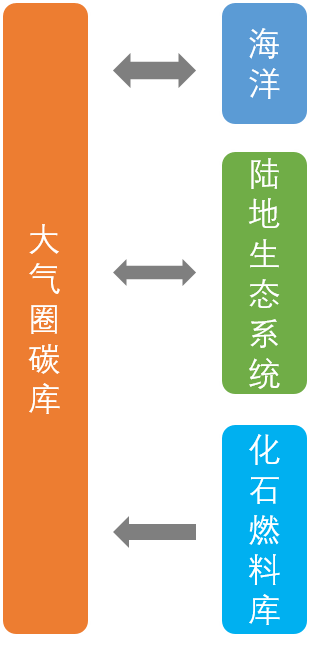
\includegraphics[width=0.9\textwidth]{carbon-cycling-structure}
    \caption{碳循环基本过程}
    \label{fig:carbon-cycling-structure}
\end{figure}

\begin{figure}[!htbp]
    \centering
    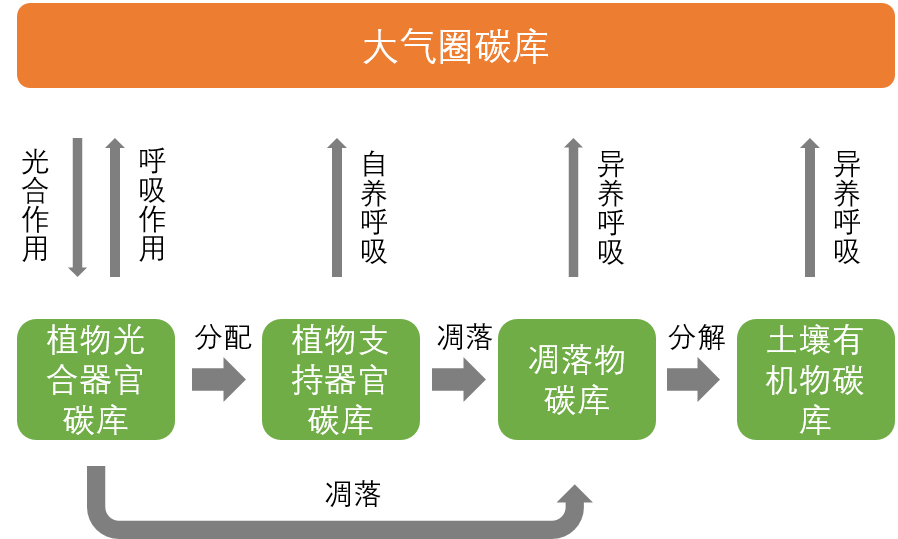
\includegraphics[width=0.9\textwidth]{land-carbon-cycling-structure}
    \caption{陆地生态系统碳循环基本过程}
    \label{fig:land-carbon-cycling-structure}
\end{figure}

\begin{figure}[!htbp]
    \centering
    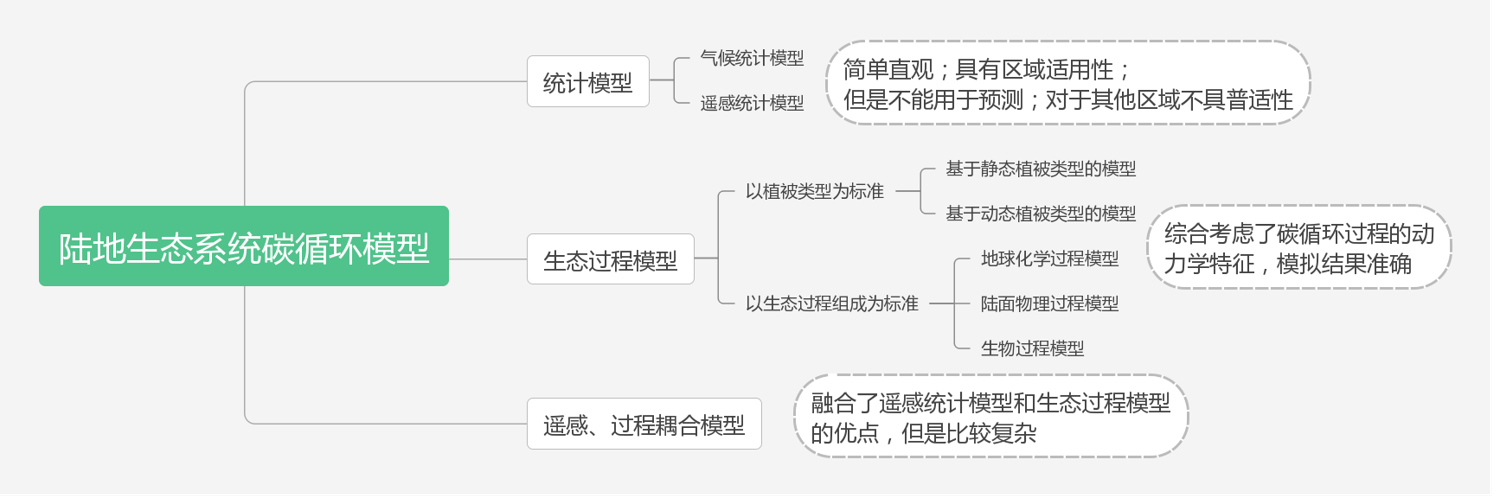
\includegraphics[width=0.9\textwidth]{carbon-model-class}
    \caption{碳循环模型分类}
    \label{fig:carbon-model-class}
\end{figure}

陆地生态系统碳循环模型从机理上可分为统计模型、生态过程模型和遥感、过程耦合模型,如图~\ref{fig:carbon-model-class}所示。
统计模型可分为气候统计模型和遥感统计模型。其中气候统计模型主要通过在温度、降水等气候因子与植被净初级生产力(Net Primary Productivity,NPP)的实测数据之间建立回归方程,代表性的有Miami模型(曼阿密模型)、Chikugo模型(筑后模型)和Thornth-waite Memorial模型(桑斯维特纪念模型);
遥感统计模型是基于遥感光谱指数建立的模型。由于总初级生产力(GPP)与截留光合有效辐射量和辐射的光合利用效率(LUE)成正比,而截留光合有效辐射与总光合有效辐射(PAR)和光合有效辐射截留率(FPAR)成正比。其中PAR可以通过气候学方法计算得到,FPAR可以通过遥感方法得到,因此,GPP可以表达为公式~\ref{eq:GPP},NPP可以表达为公式~\ref{eq:NPP}

\begin{align}
    &GPP(FPAR, PAR) = FPAR \cdot PAR \cdot LUE \cdot f(T, W, CO_2)
    \label{eq:GPP}  \\
    &NPP = GPP - R_a
    \label{eq:NPP}
\end{align}

其中,$f(T, W, CO_2)$表示温度T、土壤湿度W和大气中$CO_2$浓度对辐射的诗集光合利用效率的影响;$R_a$表示自养呼吸;代表性的模型有CASA、GLO-PEM、TURC、SIB2等
% 遥感统计模型主要通过遥感光谱指数(如NDVI)与植被净初级生产力、生物量等数据间的相关关系进行统计回归。
统计模型简单直观,具有较强的区域适用性,但其完全依赖于地面观测数据,对于不同的区域,模型不具备普适性和推广性。同时统计模型没有考虑陆地生态系统碳循环过程的内部机理,无法揭示生态系统与环境间的相互影响关系,不能用于对未来的预测研究~\cite{袁文平2014陆地生态系统植被生产力遥感模型研究进展}~\cite{谢馨瑶2018大尺度森林碳循环过程模拟模型综述}。

生态过程模型按照是否考虑实际环境对植被功能类型、组成和结构的影响分为基于动态植被类型的模型和基于静态植被类型的模型~\cite{王绍刚2008森林碳循环模型方法研究进展}~\cite{王萍2009基于}~\cite{毛留喜2006陆地生态系统碳循环模型研究概述},按照涉及到的机理类型分为地球化学过程模型、陆面物理过程模型和生物过程模型~\cite{谢馨瑶2018大尺度森林碳循环过程模拟模型综述}。过程模型由于其综合考虑了碳循环过程的动力学特征,结合了气候、土壤和植被生理生态参数,以及陆地生态系统与大气、海洋之间的相互作用,模拟结果相对来说更加准确,逐渐占据了主导地位。图~\ref{fig:DGVMs-structure}是生态过程模型的典型结构,其中冠层物理主要包括辐射传输、能量平衡、水平衡和气溶胶动力等过程,冠层生理主要用于计算光合作用和气孔导度,土壤物理包括能量平衡、水平衡和土壤温度等过程,自养呼吸主要指植被的维持呼吸和生长呼吸,异氧呼吸则指土壤呼吸和枯枝层分解,植被生理主要包括同化物分配和组织流转等过程,营养循环主要指碳、氮循环,植被竞争包括光竞争、水竞争和空间竞争,干扰过程主要涉及火灾、采伐( 或收割) 、林隙、热胁迫、干旱胁迫、背景胁迫( 如接近植被生命年限,死亡不可避免) 等,萌生过程主要指植被幼苗或种子在自然环境下的成活或萌发过程。生态过程模型的输入数据一般包括气象数据、CO2浓度数据、土壤质地数据、高程数据和植被功能类型数据等。

\begin{figure}[!htbp]
    \centering
    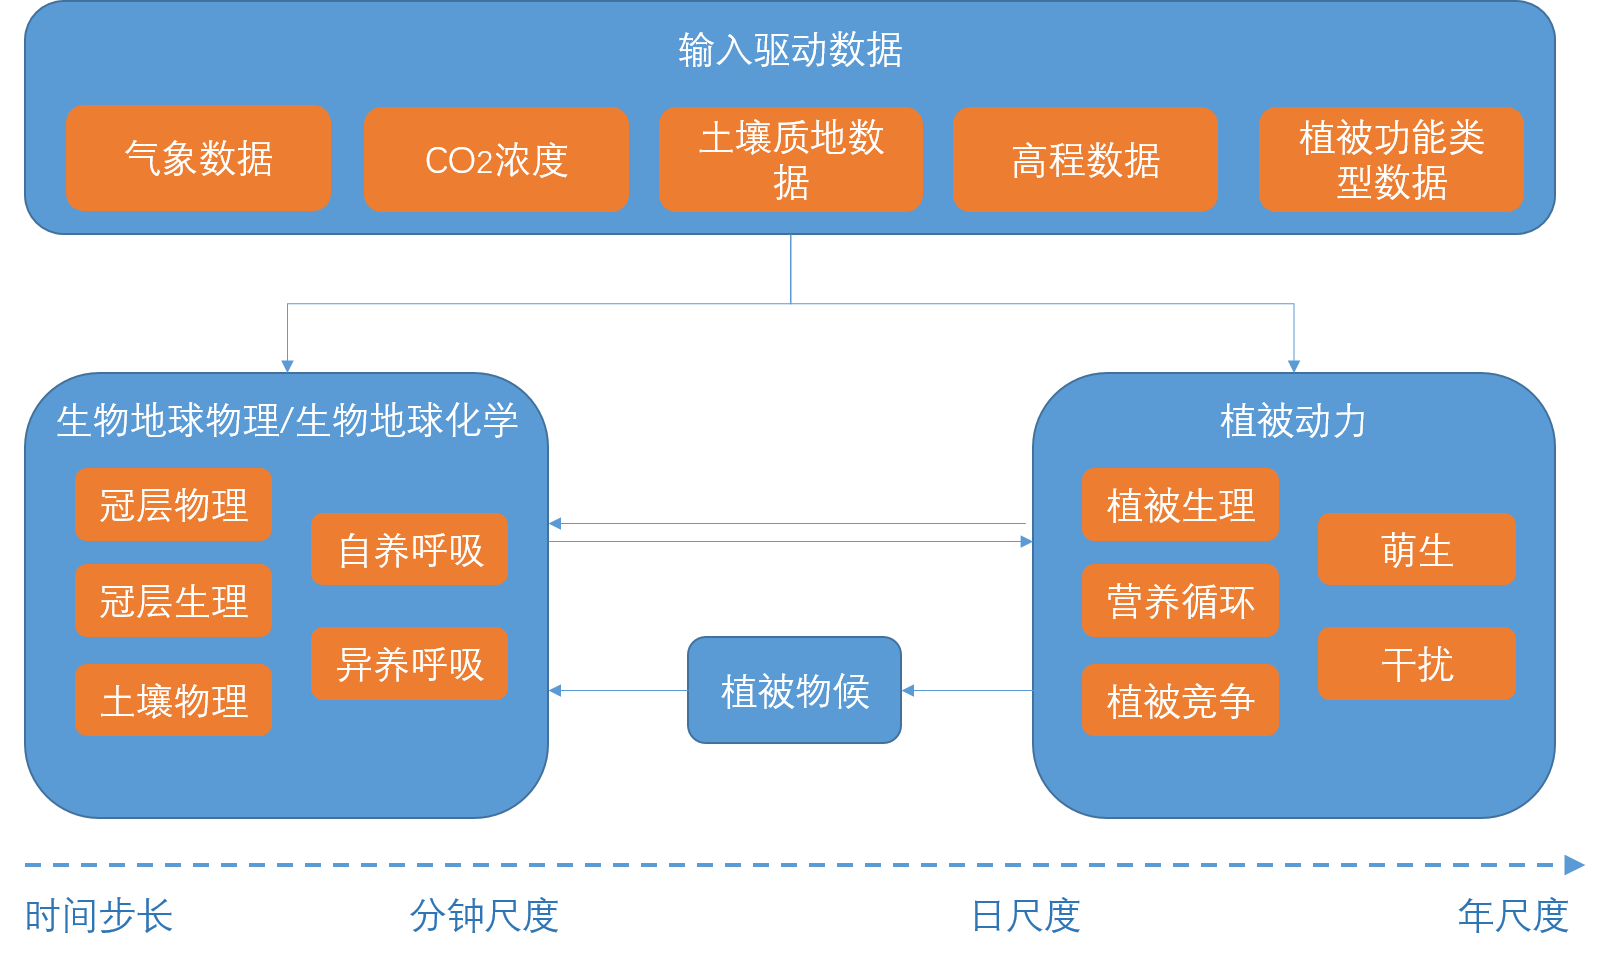
\includegraphics[width=0.9\textwidth]{DGVMs-structure}
    \caption{生态过程模型的典型结构}
    \label{fig:DGVMs-structure}
\end{figure}

遥感、过程耦合模型通过将遥感观测数据(如叶面积指数LAI)同化到模型之中,来提高模型模拟的精度(张延龙,2015),他融合了遥感统计模型和生态过程模型的优点,可以反映区域和全球尺度的NPP空间分布和变化~\cite{朱文泉2005陆地植被净初级生产力计算模型研究进展}。但由于遥感、过程耦合模型难度过大,在应用时不太方便。

综合分析三类模型的优缺点后,本文选取了IBIS、Biome-BGC、LPJ三个具有代表性的生态过程模型,在全球尺度上进行模拟和对比分析。

\subsection{IBIS, Biome-BGC, LPJ模型简介}
% 主要介绍这三个模型为何作为该类模型的代表
\subsubsection{IBIS模型}
% 起源、原理、结构、适用条件、输入数据、运行模式
\paragraph{模型简介} IBIS全称为集成生物圈模拟器(Integrated BIosphere Simulator),由美国威斯康星——麦迪逊大学Foley等~\cite{foley1996integrated}提出,随后,Kucharik等~\cite{kucharik2000testing}于2000年对其进行了改进,现在最新版本是IBIS 2.6。模型包括地表模块、土壤地球生物化学模块、植被物候模块和植被动态模块5个模块,属于动态植被类型模型。IBIS模型综合考虑了地球化学过程、地球物理过程和植被动态过程,能够耦合大气环流模式,在时间上适用于跨度从秒到数百年的碳循环过程,在空间上适用于区域尺度和全球尺度。

\paragraph{模型改进} IBIS模型的输入数据包括日分辨率的气象数据(平均温度、最大温度、最小温度、相对湿度、风速和云量)、土壤质地数据(沙粒含量、黏粒含量和粉粒含量)、植被功能类型(PFT)、网格点的经纬度。IBIS模型将植被功能类型分类及其参数如表~\ref{tab:IBIB-PFT}所示,其他详细参数见Foley等~\cite{foley1996integrated},Kucharik等~\cite{kucharik2000testing}

\begin{table}[!htbp]
    \centering
    \caption{IBIS模型植被功能类型及其生物量转换时间、碳分配系数及比叶面积}
    \label{tab:IBIB-PFT}
    \begin{threeparttable}
        \begin{tabular}{l|cccccc}
            \toprule[1.5pt] 
            \multirow{2}{*}{\textbf{植被功能类型}} & \multicolumn{3}{c}{\textbf{生物量转换时间}} & \multicolumn{2}{c}{\textbf{碳分配系数}} & \multirow{2}{*}{\textbf{比叶面积}} \\ 
            \cmidrule(lr){2-4} \cmidrule(lr){5-6}
            & \textbf{叶} & \textbf{根} & \textbf{干} & \textbf{叶} & \textbf{根} &  \\ 
            \midrule[1.5pt]
%            热带阔叶常绿林& 
%            热带落叶干旱落叶林
            温带常绿针叶&    2.50 & 1.00 & 50.00 & 0.30 & 0.40 & 25 \\ 
            温带落叶阔叶&    1.00 & 1.00 & 50.00 & 0.30 & 0.20 & 26 \\ 
            温带落叶针叶&    1.00 & 1.00 & 50.00 & 0.30 & 0.20 & 25 \\ 
            寒温带常绿针叶&  2.50 & 1.00 & 100.00 &0.30  & 0.40 &25  \\ 
            寒温带落叶阔叶&  1.00 & 1.00 & 100.00 &0.30  & 0.20 &25  \\ 
            寒温带落叶针叶&  1.00 & 1.00 & 100.00 &0.30  & 0.20 &25  \\ 
            落叶灌木&        1.00 & 1.00 & 5.00 & 0.45 &0.35  &  23\\ 
            草本&           1.50 & 1.00 & 0.00 &  0.45& 0.55 & 23 \\ 
            \bottomrule[1.5pt]
        \end{tabular}
        \begin{tablenotes}
            \footnotesize
            \item 数据来源于Foley等~\cite{foley1996integrated}、Kurcharik等~\cite{kucharik2000testing}
          \end{tablenotes}
    \end{threeparttable}
\end{table}

% 温带常绿针叶林&  &  &  &  &  &  \\ 
% 温带针阔叶混交林&  &  &  &  &  &  \\ 
% 温带硬阔叶林&  &  &  &  &  &  \\ 
% 温带软阔叶林&  &  &  &  &  &  \\ 
% 蒙古栎林&  &  &  &  &  &  \\ 
% 温带杂木林&  &  &  &  &  &  \\ 
% 寒温带兴安落叶松林&  &  &  &  &  &  \\ 
% \bottomrule[1.5pt] 

\subsubsection{Biome-BGC模型}
\paragraph{模型简介} Biome-BGC模型由美国蒙拿大大学森林学院陆地动态数值模拟团队(Numerical Terradynamic Simulation Group,NTSG)基于FOREST-BGC模型改进而来,广泛应用于模拟植被、凋落物、土壤中的碳、氮、水等物质的循环过程~\ref{Thornton2001Modeling}。模型使用静态植被类型,属于生物地球化学循环模型,包括的生理生态过程有光合作用、蒸散发、生态系统呼吸、分解、光合产物的分配以及植物的死亡,基本原理是物质和能量守恒定律,即进入生态系统中的武陟和能量,等于离开生态系统的与生态系统中累积的之和。模型的植被功能类型被分为7类:落叶阔叶林、常绿阔叶林、常绿针叶林、灌木林、落叶针叶林、C3草本植物和C4草本植物。每种植被功能类型具有许多对应的生理生态参数。该模型在时间上适用于?,在空间上适用于区域尺度和全球尺度。Biome-BGC模型的运行分为两阶段:spin-up阶段根据气象数据、工业革命前CO2浓度、碳氮水沉降值、土壤质地、生理生态参数等,进行不断迭代,直到达到给定的最大迭代年数或者状态变量达到平衡为止;常规运行阶段使用spin-up阶段运行出的结果参数、CO2浓度和气象数据模拟碳循环过程。

\paragraph{模型改进} 

\subsubsection{LPJ模型}
\paragraph{模型简介} LPJ(Lund-potsdam-Jena Model,LPJ)模型建立在Biome3模型的基础上,包括的植被生理过程包括光合作用、呼吸作用、植被冠层能量交换、土壤水平衡等。LPJ模型适用于大尺度、中尺度以及全球尺度范围内的碳循环模拟。LPJ模型的植被功能类型分为21种,其中8种木本(覆盖热带、温带和寒带,常绿、雨绿和夏绿,针叶和阔叶)(不区分林木和灌木),2种草地(覆盖热带和温带),11种作物功能类型。LPJ模型的时间分辨率是1月,Venevsky~\ref{venevsky2007sever}对运行时间步长进行了修改,时间步长变成了1天。为了和IBIS模型与Biome-BGC模型的时间分辨率一致,本文应用的是Venevsky的LPJ-Daily。LPJ模型的运行也分为两个阶段:spin-up阶段假设没有植被(全为裸土地)和生物量,进行1000年积分知道植被覆盖和土壤碳达到平衡态;常规运行阶段使用spin-up阶段运行出的平衡态作为初始值进行模拟。

\paragraph{模型改进} 

\subsubsection{三个模型的特征对比}
% 表

\section{陆地生态系统碳循环数据资源}
~\label{sec:model-data}
本文所选的三个模型均以网格点为基本模拟单位,针对全球范围内的区域,本文使用$0.5^{\circ} \times 0.5^{\circ}$的经纬网划分格点,并筛选去除海洋和裸土地的格点,最终在全球范围内共有40595个格点。

如前文所分析,生态过程模型一般都需要气象数据集、土壤数据集和植被功能类型数据集,而在进行对比时,要确保使用相同的通用数据集。而由于不同模型对这些数据在时空分辨率、植被类型等方面的要求不同,因此,本文采用相同的数据域,针对每个模型的特殊要求,对原始数据进行数据处理。

\subsection{气象数据集}
本文采用MERRA 2(Modern Era Retrospective-analysis for Research and Applications 2)气象数据集,MERRA是NASA为卫星提供的在大气再分析资料,致力于天气和气候时间尺度与水循环相关研究,具有较高的空间分辨率和较完整的时间序列范围,气象要素包括平均温、最高温、最低温、相对湿度、降水量、风速和云量。本文的数据时间范围从1982年到2013年共32年,以日为时间分辨率。数据原始空间分辨率为$0.625^{\circ} \times 0.5^{\circ}$,对其进行重采样转换为$0.5^{\circ} \times 0.5^{\circ}$,以符合全球离散网格点的空间分布。

\subsection{土壤数据集}
主要包括土壤的颗粒组成成分,即沙粒含量、黏粒含量、粉粒含量、土壤深度,由中山大学土壤——大气相互作用研究组开发~\ref{shangguan2014global}。数据的空间分辨率为$0.0085^{\circ} \times 0.0107^{\circ}$,对其进行重采样转换为$0.5^{\circ} \times 0.5^{\circ}$。数据详情参考 \href{http://globalchange.bnu.edu.cn/research/soilw}{http://globalchange.bnu.edu.cn/research/soilw}

\subsection{植被功能类型数据集}
% 植被功能类型使用
生态过程模型普遍采用植被功能类型作为植被基本处理单元,本文所选的三个模型也是如此。由于这三个模型内部对植被功能类型的划分不同,因此对原始数据进行类型映射,如表~\ref{tab:IBIS-PFT-map}, ~\ref{tab:Biome-BGC-PFT-map}, ~\ref{tab:LPJ-PFT-map}所示,分别为三个模型的植被功能类型映射表。

\begin{table}[!htbp]
    \centering
    \caption{IBIS模型植被功能类型映射表}
    \label{tab:IBIB-PFT-map}
    \begin{threeparttable}
        \begin{tabular}{lcccccc}
            \toprule[1.5pt]
            \multirow{2}{*}{\textbf{植被功能类型}} & \multicolumn{3}{c}{\textbf{生物量转换时间}} & \multicolumn{2}{c}{\textbf{碳分配系数}} & \multirow{2}{*}{\textbf{比叶面积}} \\ 
            \cmidrule(lr){2-4} \cmidrule(lr){5-6}
            & \textbf{叶} & \textbf{根} & \textbf{干} & \textbf{叶} & \textbf{根} &  \\ 
            \midrule[1.5pt]
            \bottomrule[1.5pt]
        \end{tabular}
        \begin{tablenotes}
            \footnotesize
            \item[]数据来源于Foley等~\cite{foley1996integrated}
        \end{tablenotes}
    \end{threeparttable}
\end{table}

\begin{table}[!htbp]
    \centering
    \caption{Biome-BGC模型植被功能类型映射表}
    \label{tab:Biome-BGC-PFT-map}
    \begin{threeparttable}
        \begin{tabular}{lcccccc}
            \toprule[1.5pt] 
            \multirow{2}{*}{\textbf{植被功能类型}} & \multicolumn{3}{c}{\textbf{生物量转换时间}} & \multicolumn{2}{c}{\textbf{碳分配系数}} & \multirow{2}{*}{\textbf{比叶面积}} \\ 
            \cmidrule(lr){2-4} \cmidrule(lr){5-6}
            & \textbf{叶} & \textbf{根} & \textbf{干} & \textbf{叶} & \textbf{根} &  \\ 
            \midrule[1.5pt]
            \bottomrule[1.5pt]
        \end{tabular}
        \begin{tablenotes}
            \footnotesize
            \item[]数据来源于Foley等~\cite{foley1996integrated}
        \end{tablenotes}
    \end{threeparttable}
\end{table}

\begin{table}[!htbp]
    \centering
    \caption{LPJ模型植被功能类型映射表}
    \label{tab:LPJ-PFT-map}
    \begin{threeparttable}
        \begin{tabular}{lcccccc}
            \toprule[1.5pt] 
            \multirow{2}{*}{\textbf{植被功能类型}} & \multicolumn{3}{c}{\textbf{生物量转换时间}} & \multicolumn{2}{c}{\textbf{碳分配系数}} & \multirow{2}{*}{\textbf{比叶面积}} \\ 
            \cmidrule(lr){2-4} \cmidrule(lr){5-6}
            & \textbf{叶} & \textbf{根} & \textbf{干} & \textbf{叶} & \textbf{根} &  \\ 
            \midrule[1.5pt]
            \bottomrule[1.5pt]
        \end{tabular}
        \begin{tablenotes}
            \footnotesize
            \item[]数据来源于Foley等~\cite{foley1996integrated}
        \end{tablenotes}
    \end{threeparttable}
\end{table}

\subsection{通量观测数据集}
全球通量观测网络(FLUXNET)是一个以全球广泛分布的通量塔为基础的全球通量观测网络。通量观测站点遍布世界主要国家,在北美、欧洲、亚洲、非洲都有它的区域网络存在(如亚洲通量网AsiaFlux、美洲通量网AmeriFlux、中国通量网ChinaFlux)。到如今为止,累计有800多个活跃和历史的通量测定站点,分布在全球大部分气候空间和代表性生物群系中。覆盖的植被功能类型包括热带森林、温带针叶和阔叶森林、寒带森林、农田、草原、灌木丛、苔原和湿地。它在全球范围内连续测量大气状态变量,如温度、湿度、风速、降雨量、大气二氧化碳、植被生产力、生物量等。本文使用的是La Thuile数据集,包括站点每天的温度、降水、光合有效辐射比例(FPAR)、GPP、NEP,共计有231个通量观测站点,累计900余个站点$\cdot$年次数据,作为观测数据集与模型模拟的结果进行站点尺度上的对比。站点分布如图~\ref{fig:Thuile-site-POI}所示。

\begin{figure}[!htbp]
    \centering
    %\includegraphics[width=0.9\textwidth]{Thuile-site-POI}
    \caption{La Thuile观测站点分布}
    \label{fig:Thuile-site-POI}
\end{figure}

\begin{table}[!htbp]
    \centering
    \caption{站点植被功能类型统计表}
    \label{tab:site-PFT-stat}
    \begin{threeparttable}
        \begin{tabular}{c}
            \toprule[1.5pt] 
            \midrule[1.5pt]
            \bottomrule[1.5pt]
        \end{tabular}
    \end{threeparttable}
\end{table}

\subsection{MODIS GPP/NPP数据集}
MODIS MOD17 A3提供了时空连续的遥感GPP/NPP产品,MODIS/GPP产品以其他MODIS产品为基础计算而得,时间范围从2000年到2015年,时间分辨率为8天,空间分辨率为$0.0083^{\circ} \times 0.0083^{\circ}$,对其进行重采样转换为$0.5^{\circ} \times 0.5^{\circ}$。本文使用MODIS GPP/NPP 数据集作为全球尺度上的对比验证数据集,与三个模型模拟的结果进行对比分析。

\subsection{其他数据集}
模型还需要网格点的物理常量数据,包括有格点高程数据、短波反射率等。其中高程数据使用的是DEM数据

% \section{陆地生态系统碳循环模型对比方案分析和归纳}
% \subsection{基于实验协议的模型对比方案}
% % CMIP

% \subsection{可迁移、复用与重现的模型对比方案}
% % CORDEX
% % 基于虚拟机镜像/包管理器/docker

% \subsection{陆地生态系统碳循环模型对比方案总结}
% % 这一部分很重要,要明确的说明以上方案的不足之处
% % 引出我们的对比方案的优点和设计
% % 这是立题之本

% 传统的模型对比框架是以数据为基础,不考虑生产数据即模型模拟的过程。

\section{本章小结}
\chapter{陆地生态系统碳循环模型开放式对比框架}
\label{cha:3}

根据第\ref{chap:model}章的分析,陆地生态系统碳循环模型具有种类多样、参数复杂、难以应用的特点,模拟过程参与的要素众多(如GPP、NPP、NEP、Biomass、LAI等),模拟站点丰富,数据需求量大、难以搜集。这些因素都共同阻碍了碳循环模型的应用和发展,开展模型对比工作往往十分艰巨,像CMIP项目那样,各个模式开发组共同参与进来才能更顺利地完成。但是传统的对比框架也面临着一些问题,它将模型计算和对比过程都放在本地计算机运行,模型难以共享和重用,对比过程不够公开,换一套数据或研究区域就难以重现或重复,这些都是由于基于本地计算的对比框架所导致的。针对这一问题,本章旨在设计一个开放式的对比框架,支持将各种对比资源以微服务的形式开放地接入进来,实现可共享、可重用、公开化的陆地生态系统碳循环模型的对比。

本章首先分析了陆地生态系统碳循环模型的对比情景,并从中归纳总结出“对比话题——对比方案——对比任务”的三部流程;其次详细探讨了对比过程中的需要接入的地理资源组件库,包括有模型服务资源库、数据服务资源库、单位量纲资源库、数据处理服务资源库、对比服务资源库,并设计了对应接口来满足相应资源的接入,实现了对比资源的标准一致性和可扩展性;然后设计了分布式的网络系统架构,将整体复杂的系统功能分割为三部分,实现了功能的解耦和系统的稳定和;最后通过科学工作流引擎支持网络环境下对比流程地自动化执行。
本系统的整体架构如图\ref{fig:CMIP-architecture}所示。

\begin{figure}[!htbp]
    \centering
    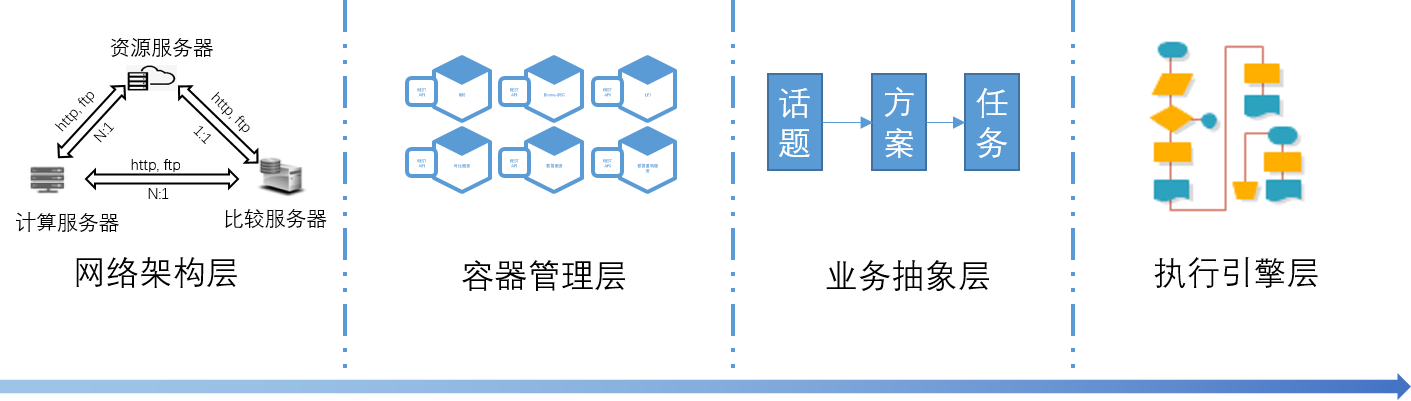
\includegraphics[width=.85\textwidth]{CMIP-architecture}
    \caption{陆地生态系统碳循环模型开放式对比框架}
    \label{fig:CMIP-architecture}
\end{figure}

\section{陆地生态系统碳循环模型对比情景和业务分析归纳}
\subsection{对比情景分析和总结}
\label{sec:scene}
% TODO 根据实验前提,详细介绍对比方案中的情景
陆地生态系统碳循环模型的应用广泛,未来的发展方向也主要停留在以下几个关键问题上:
\begin{enumerate}[(1)]
\item \textbf{陆地生态系统碳循环模型对历史植被生长的模拟}

在CMIP5和CMIP6的设计中,都设定了历史情景模拟,即根据历史时期的太阳常数、温室气体浓度、臭氧浓度、气溶胶浓度等观测资料来模拟气候因子,是气候系统模式参与CMIP项目的必要实验。而陆地生态系统碳循环模型作为气候系统模式机理中的一个子过程,也需要对历史时期进行模拟,来评估模型的模拟能力。历史情景分析是最常见的模拟情景,本文将在实验案例中详细介绍模拟结果。

\item \textbf{陆地生态系统碳循环模型的未来预测情景}
% 参考顾雪峰博士论文

在CMIP5和CMIP6中也设定了未来气候情景分析,即预测未来CO2浓度和气候因子(温度、降水)等指标的变化情况。在陆地生态系统碳循环模型对植被生产力的模拟方面,未来情景设定为气温、降水、CO2浓度的变化对植被生产力的影响,即研究陆地生态系统碳循环模型对气候变化(如温度、降水等)和CO2浓度的响应。CMIP5对未来100年全球气候变化的研究结果表明,全球平均气温从1990年到2100年上升$1.4\sim5.8^{\circ}C$~\cite{王绍武1995未来}~\cite{秦大河2003气候变化的事实与影响及对策};全球平均降水将会增加,但是降水格局也发生了很大的变化,即有些地区降水增加,有些地区降水减少;未来大气CO2浓度最大升高到当前的2倍~\cite{griggs2002climate}。根据这些预测的未来气候情景,对温度、降水和CO2浓度的变化做出变量组合,表~\ref{tab:future-scene}可以表示一种参考的组合。

% \hspace*{2cm}
\begin{table}[!htbp]
    \centering
    \caption{陆地生态系统碳循环模型的未来预测情景参数设定}
    \label{tab:future-scene}
    \begin{threeparttable}
        \begin{tabular}{lll}
            \Xhline{2pt}
            {\textbf{因素}} & {\textbf{值}} & {\textbf{标记}} \\
            \Xhline{2pt}
            \multirow{4}{*}{\textbf{气温}} & 不变 & $Temp_{0}$ \\
            & +2$^{\circ}C$ & $Temp_{1}$ \\
            & +4$^{\circ}C$ & $Temp_{2}$ \\
            & +6$^{\circ}C$ & $Temp_{3}$ \\
            \hline
            \multirow{7}{*}{\textbf{降水}} & 不变 & $Prec_0$ \\
            & 全年+10\% & $Prec_{+10}$ \\
            & 全年-10\% & $Prec_{-10}$ \\
            & 全年+20\% & $Prec_{+20}$ \\
            & 全年-20\% & $Prec_{-20}$ \\
            & 全年+30\% & $Prec_{+30}$ \\
            & 全年-30\% & $Prec_{-30}$ \\
            \hline
            \multirow{2}{*}{\textbf{CO2浓度}} & 不变 & $CO2_0$ \\
            & 两倍 & $CO2_{*2}$ \\
            \hline
            \multirow{4}{*}{\textbf{多因素}} & 温度增加、降水增加 & $Temp_{3} + Prec_{+10}$ \\
            & 温度增加、降水减少 & $Temp_{3} + Prec_{-10}$ \\
            & 温度增加、降水增加、CO2浓度翻倍 & $Temp_{3} + Prec_{+10} + CO2_{*2}$ \\
            & 温度增加、降水减少、CO2浓度翻倍 & $Temp_{3} + Prec_{-10} + CO2_{*2}$\\
            \Xhline{2pt}
        \end{tabular}
    \end{threeparttable}
\end{table}

\item \textbf{陆地生态系统碳循环模型的敏感性分析情景}
% 和对温度、降水、CO2的响应比较像,这里针对的是模型参数

在模型评价中,不确定分析研究的是模型参数、驱动变量等不确定性因素发生变化时,所引起的模型模拟结果的变化和变化程度。敏感性分析是模型不确定分析的一种常用方法,它用来研究和预测不确定性因素发生变化时,对模型结果影响程度的分析方法,又称为灵敏度分析。敏感性分析通常用来评估模型参数的重要性,分为总体敏感性分析和局部敏感性分析。局部敏感性分析相对来说更加简单,他分析单个模型参数对模拟结果的影响,但是他忽略了模型之间多个参数的相互作用对模拟结果的影响;全局敏感性分析不仅分析单个参数对模拟结果的影响,还分析参数之间的相互作用对结果的总影响,但计算起来比较复杂,耗费时间。
在本文中,将敏感性分析也理解为一种对比情景,即在不同的模型参数下模拟结果的对比,可以与正常模拟与观测数据的对比采用相同的对比方法。敏感性分析的情景设定需要从每个模型中选出一系列关键参数,根据参数的取值设定具体的情景,由于本文的研究重点不在于此,不做详细设定。

\item \textbf{陆地生态系统碳循环模型的参数校准情景}

碳循环模型的模拟精确度很大成分上依赖于模型参数的设定,目前在参数校准方面有人工校准和自动校准两种。人工校准通常有三种方法:对比实验、实验观测和文献查找;自动校准通过神经网络等各种模型进行校准。模型参数的校准可以理解为在不同模型参数下模型模拟结果的对比,因此可以作为对比的一种情景。

\end{enumerate}

\subsection{对比业务抽象和归纳}
% 对比分析、名词解释
% topic solution task
% 案例
% 意义:可共享 可重用
% TODO 对比方案具体点:有观测数据、无观测数据

在进行对比业务抽象和归纳之前,先对本文中的一些名字做出解释:本文将GPP、NPP、NEP、Biomass、LAI等模拟指标称之为\textbf{对比要素};将模型对比过程中所需要的所有数据称之为\textbf{对比数据集},一套对比数据集包括有输入数据集、观测数据集。其中输入数据集由气象数据集、土壤数据集、植被功能类型数据集、DEM数据集等组成,每个具体的数据集可以选择可替换的模块,如气象数据集既可以采用MERRA 2再分析资料,又可以使用CRU再分析资料。在第\ref{sec:model-data}节中具体介绍的数据本文称之为标准对比数据集,作为系统分析的基础原始数据,而在其之上参照表~\ref{tab:future-scene}对数据进行的一系列修改,比如对温度$\pm2^{\circ}C$,对降水$\pm10\%$等,本文称之为衍生对比数据集。每一个模拟情景都有一套相对应的对比数据集。本文将参与对比的模型称之为\textbf{对比参与者}。

\begin{figure}[!htbp]
    \centering
    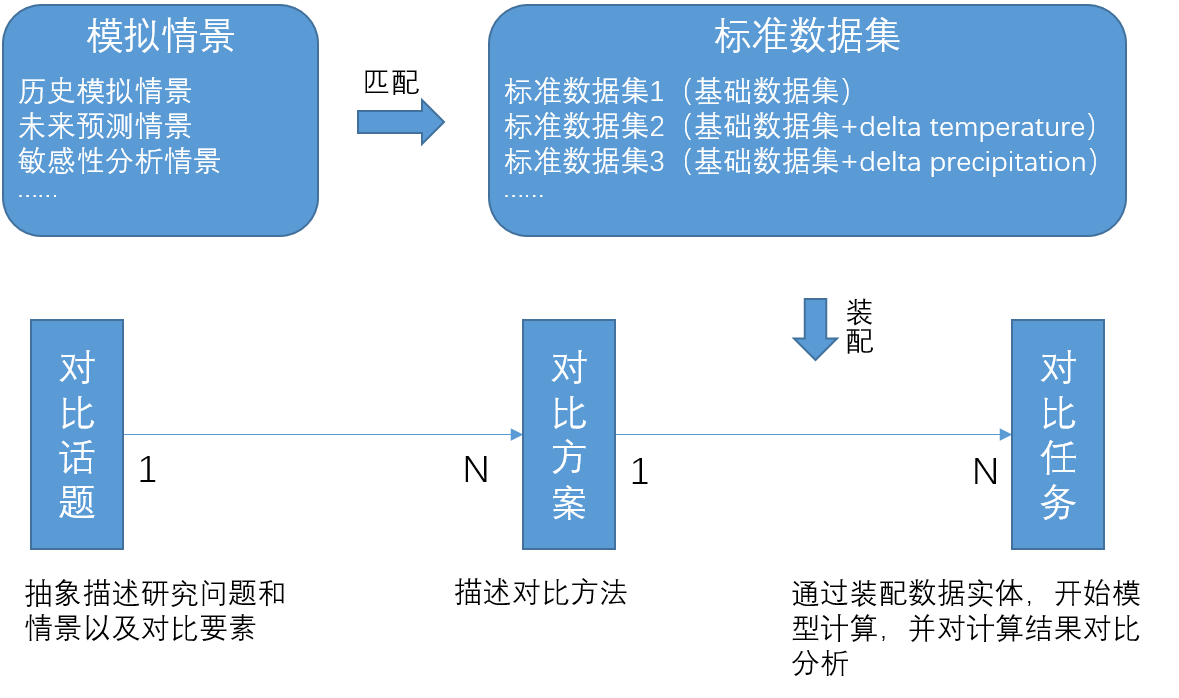
\includegraphics[width=1\textwidth]{cmip-business-abstraction}
    \caption{陆地生态系统碳循环模型对比业务抽象和归纳}
    \label{fig:cmip-business-abstraction}
\end{figure}

陆地生态系统碳循环模型在各种情景中可以归纳出三个主要关注点:研究问题、对比方法和模型运行数据的设定。这三点可以抽象为对比话题、对比方案和对比任务三个层次,如图~\ref{fig:cmip-business-abstraction}所示,对比业务的开展对应为对比话题、对比方案和对比任务创建和执行上。其中,\textbf{对比话题}中指明了研究问题、对比情景和对比要素;\textbf{对比方案}配置了对比参与者和对比方法,对比方案不包括具体的输入数据、观测数据和模拟结果,他表示的仅仅是对比的配置项,从而实现对比过程的可共享性、可重用性和可重现性;\textbf{对比任务}描述的是对比方案配置输入数据和观测数据实体的结果。模型在对比任务中开始具体的运算,并将运算结果与观测数据进行统计学对比和可视化对比。1个对比话题可以对应多个对比方案,一个对比方案通过配置不同的标准数据集可以对应多个对比任务。图~\ref{fig:ModelComparison!3-1-topic-solution-task_3}展示了对比话题、对比方案和对比任务的详细接口设计。

\begin{figure}[!htbp]
    \centering
    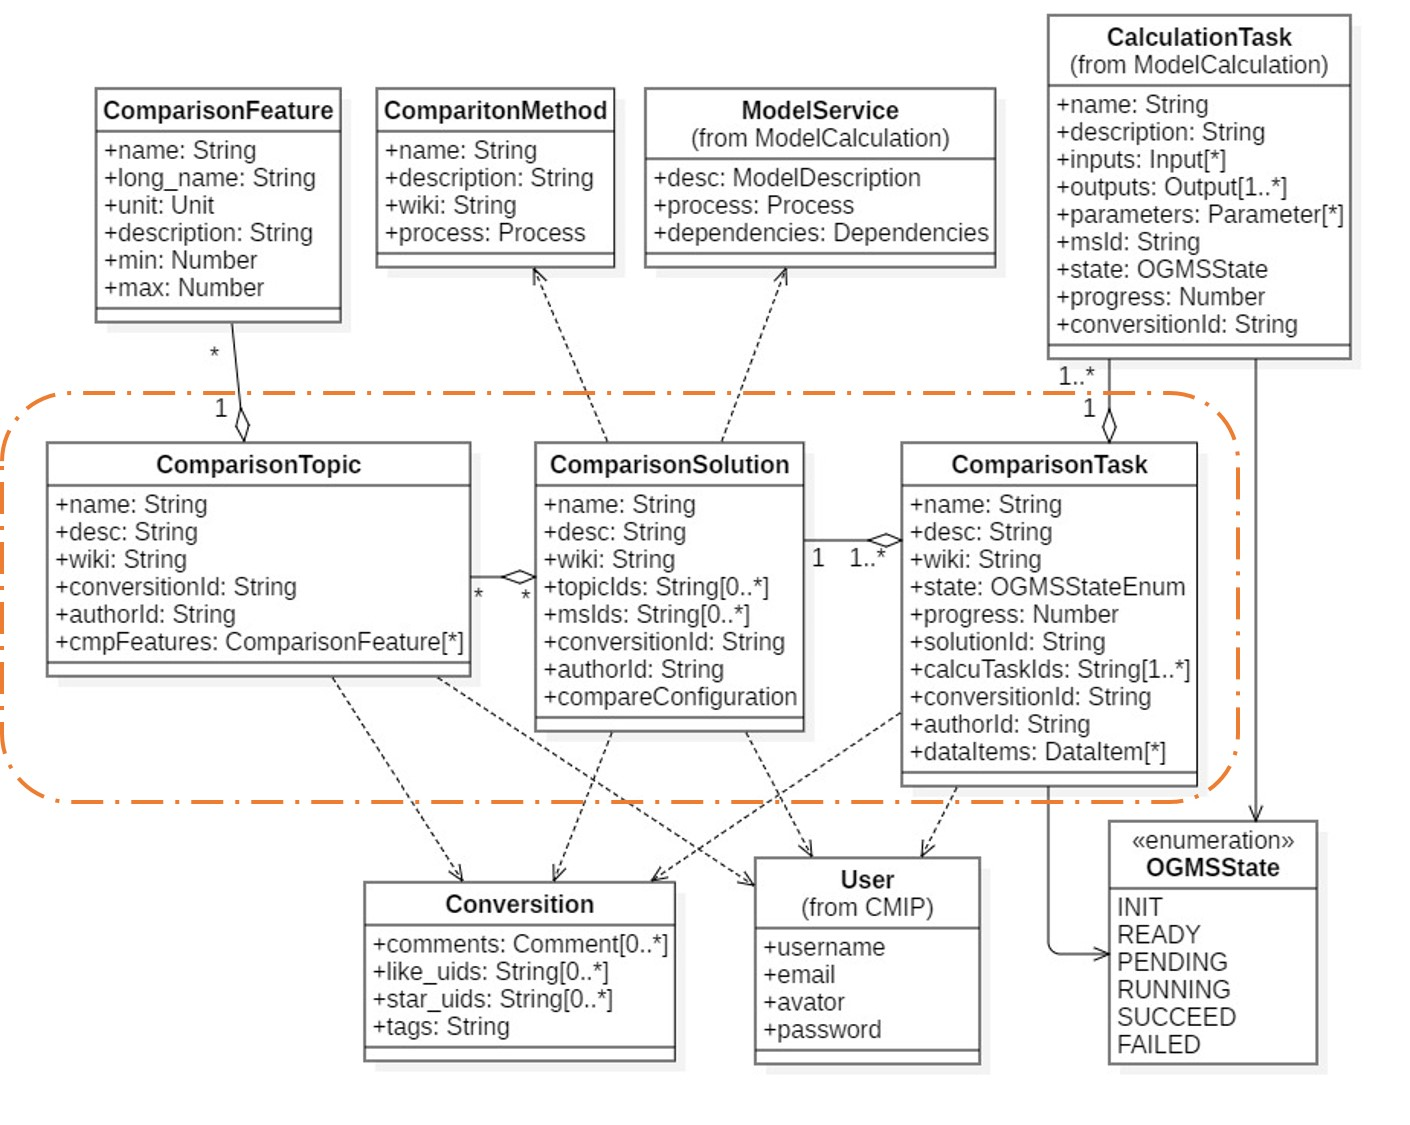
\includegraphics[width=1\textwidth]{jpg/ModelComparison!3-1-topic-solution-task_3}
    \caption{对比话题、对比方案和对比任务的接口设计UML图}
    \label{fig:ModelComparison!3-1-topic-solution-task_3}
\end{figure}

以植被生产力的对比为例,如表\ref{tab:topic-solution-task-example}所示,针对全球历史时期的植被生产力创建一个对比话题,对比要素包括有GPP、NPP、NEP等,这一个话题关联两个对比方案,其中对比参与者相同,都是IBIS、Biome-BGC和LPJ三个模型,第一个方案研究的是站点尺度,它使用的对比方法包括统计学和可视化两大类,通过配置不同的站点数据可以对应231个对比任务;第二个方案研究的是全球范围,它使用的对比方法只有可视化对比方法,只能创建一个相应的对比任务。这样的三层抽象使对比方案可共享与重用,简化了模型对比的难度,并将最后的对比结果公开发布为服务,使对比过程公开透明,更加具有可信度。

% TODO 从 pdf 导入吧
\begin{table}
    \centering
    \caption{针对全球植被生产力评估的对比话题、对比方案和对比任务}
    \label{tab:topic-solution-task-example}
    \begin{threeparttable}
        \begin{tabular}{l | l | l | l | l }
            \Xhline{1.5pt}
            \multicolumn{2}{c}{\makecell[b]{对比话题}} & \multicolumn{2}{|c|}{\makecell[b]{对比方案}} & \multicolumn{1}{l}{\makecell[b]{对比任务}} \\
            \hline
            模拟情景 & 对比要素 & \makecell{对比参与者} & \makecell{对比方法} & 数据区域 \\
            
            \Xhline{1.5pt}
            \multirow{3}{*}{历史情景} & \multirow{3}{2cm}{GPP \quad NPP \quad NEP\ } & \multirow{3}{*}{\makecell{IBIS\\Biome-BGC\\LPJ}} & \multirow{2}{*}{\makecell{统计学对比方法\\可视化对比方法}} & CN-Cha(长白山)站点 \\
            \cline{5-5}
            &  &  &  & 其他站点,共231个 \\
            \cline{4-5}
            &  &  & 可视化对比方法 & 全球 \\
            \Xhline{1.5pt}
        \end{tabular}
    \end{threeparttable}
\end{table}

\subsection{对比系统功能模块设计}
本文将系统的主要功能模块设计为如图\ref{fig:system-module},功能模块分为资源模块、对比业务模块、结果展示模块和用户模块,其中资源模块包括模型资源和数据资源,对比业务模块则对应于对比话题、对比方案和对比任务,结果展示模块基于所有对比任务的对比结果,以网站的形式发布出去。

\begin{figure}[!htbp]
    \centering
    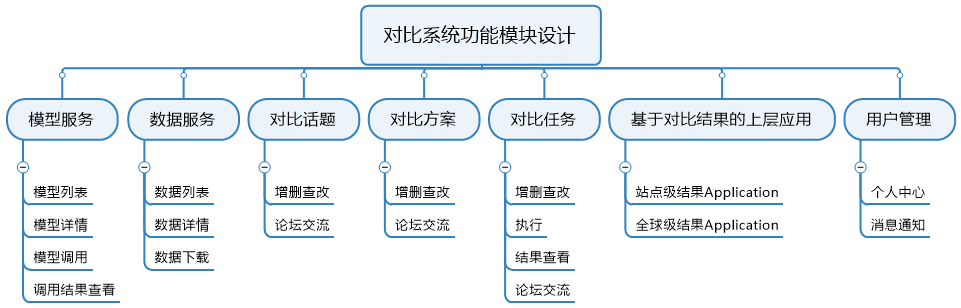
\includegraphics[width=1\textwidth]{system-module}
    \caption{对比系统功能模块设计}
    \label{fig:system-module}
\end{figure}

\section{基于服务的地理资源组件库}
GIS的发展和信息技术的发展紧密关联,随着IT技术的不断推动,GIS经历了从集成式到组件式再到基于服务的Web GIS的发展历程,其中集成式GIS功能丰富全面但系统复杂、庞大、成本高昂,而且不能与其他系统集成;组件式GIS通过多元空间数据无缝集成技术(Seamless Integration of Multisource Spatial-data,SIMS)解决了多源异构数据的访问,并且具有可扩展、可共享和可重用能力,但是组件只能应用于本地计算机;基于Web Service的Web GIS则通过定义空间数据和模型的标准描述协议,实现了数据、模型及计算资源的共享,具备可扩展性、跨平台性,使GIS真正实现大众化。

Web Service是一种服务导向架构的技术,通过Web协议提供服务,可以保证不同平台的应用程序之间可以互操作。Web Service的实现方式一般有简单对象访问协议(Simple Object Access Protocol,SOAP)和表述性状态转移(Representational State Transfer,REST)两种。REST服务在服务注册量、普及程度、响应时间、吞吐量和数据传输方面的性能都要优于SOAP服务~\cite{2015互联网上基于},因此本文选择REST服务作为技术支撑。REST服务基于HTTP协议之上,通过定义一种软件架构风格,以HTTP请求的POST、DELETE、GET和PUT方法对应对资源的增删查改操作~\cite{fielding2000architectural}。REST服务的特点是客户端——服务器端(Client-Server)架构、无状态、接口统一、系统分层等。
使用REST服务接入地理资源,可以让不同的服务器处理不同的请求,能够提高服务器的扩展性。

\subsection{模型服务资源库}
由于模型资源在编程语言(如C++、C\#、JAVA等)、存在形式(如源代码、可执行程序、DLL等)、运行交互方式(如控制台应用程序、GUI、网络服务等)、运行平台(如Windows、Linux、Unix等)等方面存在着很强的异构性,模型本身很难作为组件接入到框架下,对模型进行封装可以屏蔽这些异构性,形成标准化的模型服务。模型服务资源库由这些标准化的服务组成,它的应用模式如图~\ref{fig:model-operation}所示,其中每一步都通过HTTP协议传输,其详细接口设计如表~\ref{tab:model-service-API}所示。

其中模型调用接口“/model-service/:msId/invoke”是最重要的,其请求参数如表~\ref{tab:model-invoke-API}所示,输入项、参数项、输出项的id从“/model-service/:msId”接口返回的描述文档中可以获取,输入项的“value”是上传到服务器返回的数据id,参数项的“value”是Number或String类型的值,输出项的“value”不用填写。发送请求后,如果调用成功,则返回运行记录的id,凭此id可以通过“/model-service/record/:recordId”接口请求模型的运行记录,并从中获取运算的结果。

模型服务资源库屏蔽了模型的异构性,简化了模型的使用难度,不同的模型资源具有相同的地位和角色,都看作为对比参与者,在对比框架下,能够可扩展地加入到对比方案中。

\begin{figure}[!htbp]
    \centering
    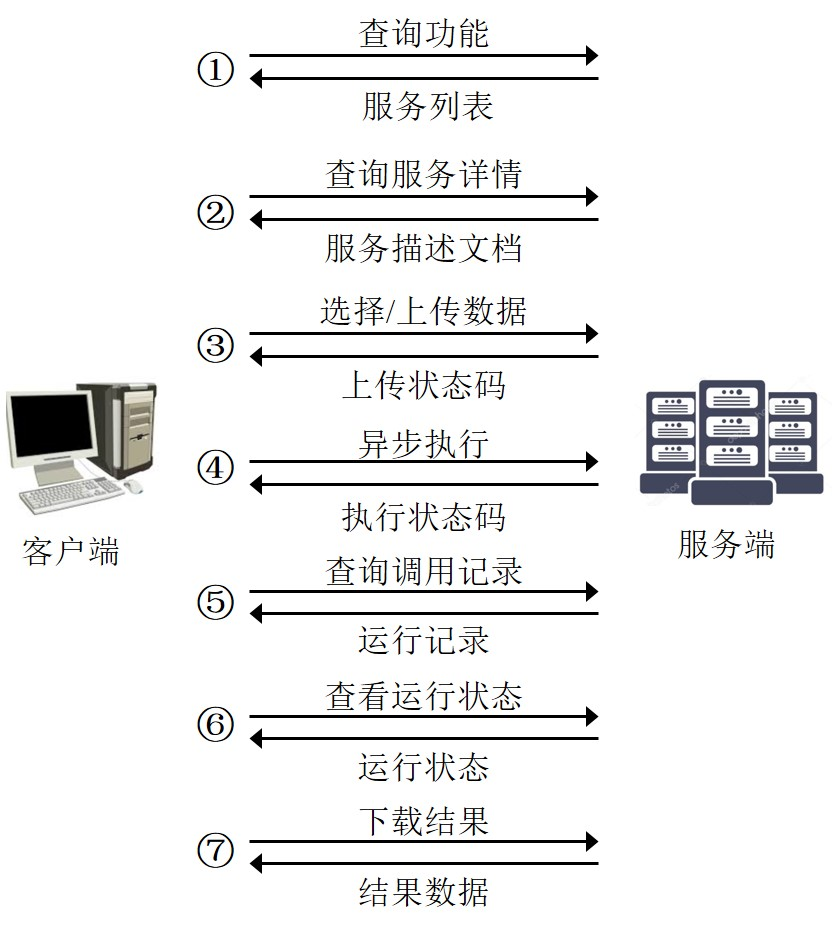
\includegraphics[width=.8\textwidth]{model-operation}
    \caption{模型服务交互模型}
    \label{fig:model-operation}
\end{figure}

\begin{table}[!htbp]
    \centering
    \caption{模型服务API}
    \label{tab:model-service-API}
    \begin{tabular}{llll}
        \Xhline{1.5pt}
        名称 & 请求方式 & 返回 & 说明 \\
        \Xhline{1.5pt}
        /model-service & GET & 模型服务列表 & 查询模型服务 \\
        /model-service/:msId & GET & 模型描述文档 & 查询模型详情 \\
        /model-service/:msId/invoke & POST & 状态码 & 运行模型 \\ 
        /model-service/record & GET & 运行记录列表 & 查询模型运行记录 \\
        /model-service/record/:recordId & GET & 运行记录 & 查询运行记录 \\
        \Xhline{1.5pt}
    \end{tabular}
\end{table}

\begin{table}[!htbp]
    \centering
    \caption{模型调用接口请求参数}
    \label{tab:model-invoke-API}
    \begin{tabular}{lll}
        \Xhline{1.5pt}
        参数 & 结构 & 描述 \\
        \Xhline{1.5pt}
        inputs 
        & 
        % \begin{minted}[tabsize=4]{js}
        $\{ "id": "data\_flag", "value": "data\_id\_you\_had\_uploaded" \}[]$
        % \end{minted}
        & 输入数据列表 \\
        parameters 
        &
        % \begin{minted}[tabsize=4]{js}
        $\{ "id": "data\_flag", "value": "parameter\_value" \}[]$
        % \end{minted}
        & 参数列表 \\
        outputs 
        &
        % \begin{minted}[tabsize=4]{js}
        $\{ "id": "data\_flag", "value": null \}[]$
        % \end{minted}
        & 输出数据列表 \\
        \Xhline{1.5pt}
    \end{tabular}
\end{table}

\subsection{数据服务资源库}
数据服务资源库由数据下载服务、数据重构服务和OGC WMS、WFS、WCS三类组成。其中数据下载服务将数据按照多种分类体系发布出去,并提供数据的相关元数据描述文档。数据在模型运行和对比时,往往并不能直接驱动程序的运行,数据重构服务对数据做出转换,它的调用交互模式和模型服务的调用类似,表~\ref{tab:data-service-API}列出了数据服务的详细接口,OGC WMS、WFS、WCS服务的接口和发布在后文第~\ref{subsubsec:OGC}节详细介绍。

\begin{table}[!htbp]
    \centering
    \caption{数据服务API}
    \label{tab:data-service-API}
    \begin{tabular}{llll}
        \Xhline{1.5pt}
        名称 & 请求方式 & 返回 & 说明 \\
        \Xhline{1.5pt}
        /data & POST & 状态码和数据id & 上传数据 \\
        /data & GET & 数据列表 & 获取数据列表 \\
        /data/:dataId & GET & 数据文件 & 下载数据 \\
        /data/:dataId/metadata & GET & 元数据文档 & 获取元数据 \\
        /data-refactor & GET & 数据重构服务列表 & 查询数据重构服务 \\
        /data-refactor/:id & GET & 重构服务描述 & 查询重构服务详情 \\
        /data-refactor/:id/invoke & POST & 状态码 & 运行重构服务 \\
        /data-refactor/record & GET & 运行记录列表 & \multicolumn{1}{m{0.3\columnwidth}}{查询重构服务运行记录} \\
        /data-refactor/record/:recordId & GET & 运行记录 & 查询运行记录 \\
        \Xhline{1.5pt}
    \end{tabular}
\end{table}

\subsection{单位量纲资源库}
单位量纲资源库由模型运算过程中涉及到的单位和量纲组成,如图~\ref{fig:ModelComparison!3-2-unit-dimension_5}所示,量纲类Dimension由7个基本物理量组成,他们分别是长度($L$)、质量($M$)、时间($T$)、电流($I$)、温度($\Theta$)、物质的量($N$)、发光强度($J$)。而单位类Unit则由这7个基本物理量组合表示(对于无量纲的单位为空),它也可以是自定义的单位。在对比要素类ComparisonFeature中用单位来表达它的具体物理意义,对于不同的单位表示法,可以通过量纲分析进行换算。单位量纲只有一个接口,以GET方式请求“/metrics”可以获取单位量纲列表。表~\ref{tab:std-metrics}列出了本文涉及到的对比要素及其所使用的单位。

模型在对比时模拟数据和观测数据的单位量纲一般不完全相同,以GPP为例,IBIS的输出单位是$gC m^2 d^{-1}$,Biome-BGC的输出单位是$kgC m^2 d^{-1}$,观测数据的单位是$gC m^2 d^{-1}$,在对比时,需要将单位一致化,单位量纲资源库为单位转换提供参考。

\begin{figure}[!htbp]
    \centering
    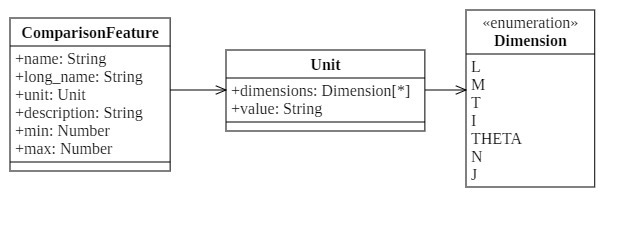
\includegraphics[width=.9\textwidth]{jpg/ModelComparison!3-2-unit-dimension_5}
    \caption{单位量纲UML图}
    \label{fig:ModelComparison!3-2-unit-dimension_5}
\end{figure}

% \renewcommand{\arraystretch}{1.5}
% TODO min and max
\begin{table}[!htbp]
    \caption{对比要素及其单位量纲}
    \label{tab:std-metrics}
    \begin{subtable}[t]{.6\linewidth}
        \centering
        \caption{陆地生态系统碳水循环要素表}
        \label{tab:c-w-feature}
        \begin{tabular}{llrrr}
            \Xhline{1.5pt}
            \textbf{名称} & \textbf{单位} & \textbf{最小值} & \textbf{最大值}  \\
            \Xhline{1.5pt}
            $GPP$ & $gC m^2 d^{-1}$ & 0 & 100 \\
            $NPP$ & $gC m^2 d^{-1}$ & 0 & 100 \\
            $NEP$ & $gC m^2 d^{-1}$ & -100 & 100 \\
            $NEE$ & $gC m^2 d^{-1}$ & -100 & 100 \\
            $Biomass$ & $gC m^2 d^{-1}$ & 0 & - \\
            $R_A$ & $gC m^2 d^{-1}$ & 0 & 100 \\
            $R_H$ & $gC m^2 d^{-1}$ & 0 & 100 \\
            $ET$ & $mm d^{-1}$ & 0 & 100\\
            $Runoff$ & $mm d^{-1}$ & - & - \\
            $LAI$ & $1$ &  & \\
            \Xhline{1.5pt}
        \end{tabular}
    \end{subtable}%
    \begin{subtable}[t]{.3\linewidth}
        \centering
        \caption{单位量纲表}
        \label{tab:unit-dimension}
        \begin{tabular}{ll}
            \Xhline{1.5pt}
            \textbf{单位} & \textbf{量纲}  \\
            \Xhline{1.5pt}
            \multirow{3}{*}{$gC m^2 d^{-1}$} & 质量($M$) \\
            & 长度($L$) \\
            & 时间($T$) \\
            \hline
            \multirow{2}{*}{$mm d^{-1}$} & 长度($L$) \\
            & 时间($T$) \\
            \Xhline{1.5pt}
        \end{tabular}
    \end{subtable}
\end{table}

\subsection{对比服务资源库}
对比服务资源库分为两类:统计学对比方法和可视化对比方法。他们都接受一条或多条数据为输入,统计学对比方法返回的是统计指标,可视化对比方法返回的是图片结果。表~\ref{tab:cmp-service-API}列出了去详细接口。

\begin{table}[!htbp]
    \centering
    \caption{对比服务API}
    \label{tab:cmp-service-API}
    \begin{tabular}{llll}
        \Xhline{1.5pt}
        名称 & 请求方式 & 返回 & 说明 \\
        \Xhline{1.5pt}
        /cmp & GET & 对比服务列表 & 查询对比服务 \\
        /cmp/:cmpId & GET & 对比服务描述文档 & 查询对比服务详情 \\
        /cmp/:cmpId/invoke & POST & 状态码 & 运行对比服务 \\ 
        /cmp/record & GET & 对比记录列表 & 查询对比服务运行记录 \\
        /cmp/record/:recordId & GET & 对比结果 & 查询对比结果 \\
        \Xhline{1.5pt}
    \end{tabular}
\end{table}

\section{基于微服务的分布式网络架构设计}
% 开放性应体现在:可共享和重用(业务流程归纳)、计算和对比过程公开化(服务化)、模型和数据资源可扩展(微服务注册和发现)、大规模计算场景下体系稳定可用(微服务LB)、自动化易用(科学工作流)
\subsection{微服务简介与应用}
% 介绍、特点、优点、应用
分布式系统是有一组通过网络进行通信、为了完成共同的任务而协调工作的计算机节点组成的系统。分布式将不同物理区域的计算资源组织整合起来,与传统的集中式相对比,分布式能够有效利用多个分布式节点上的计算能力和数据共享能力,从而提高服务端的性能。
微服务是一种分布式的系统架构风格,由Martin Fowler提出~\cite{fowler2014microservices},微服务是颗粒比较小的服务,服务之间相互独立,具有其独自的数据管理,可以被独立部署,一个大型的复杂软件可以由多个微服务组成。微服务采用UNIX的设计哲学,每种服务只做一件事,是一种松耦合的能够被独立开发和部署的无状态化服务。微服务通过服务来实现应用的组件化,微服务中将组件定义为可被独立替换和升级的软件单元,在应用架构设计中通过将整体应用切分成可独立部署的多个微服务方式进行组件化设计。

\begin{figure}[!htbp]
    \centering
    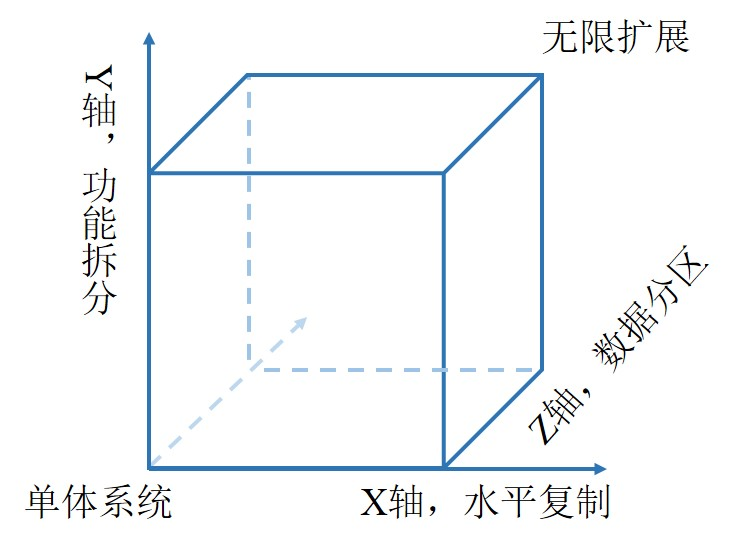
\includegraphics[width=.35\textwidth]{AKF-cube}
    \caption{AKF扩展立方体模型}
    \label{fig:AKF-cube}
\end{figure}

\begin{figure}[!htbp]
    \centering

    \subcaptionbox{微服务应用架构\label{micro-arch}}{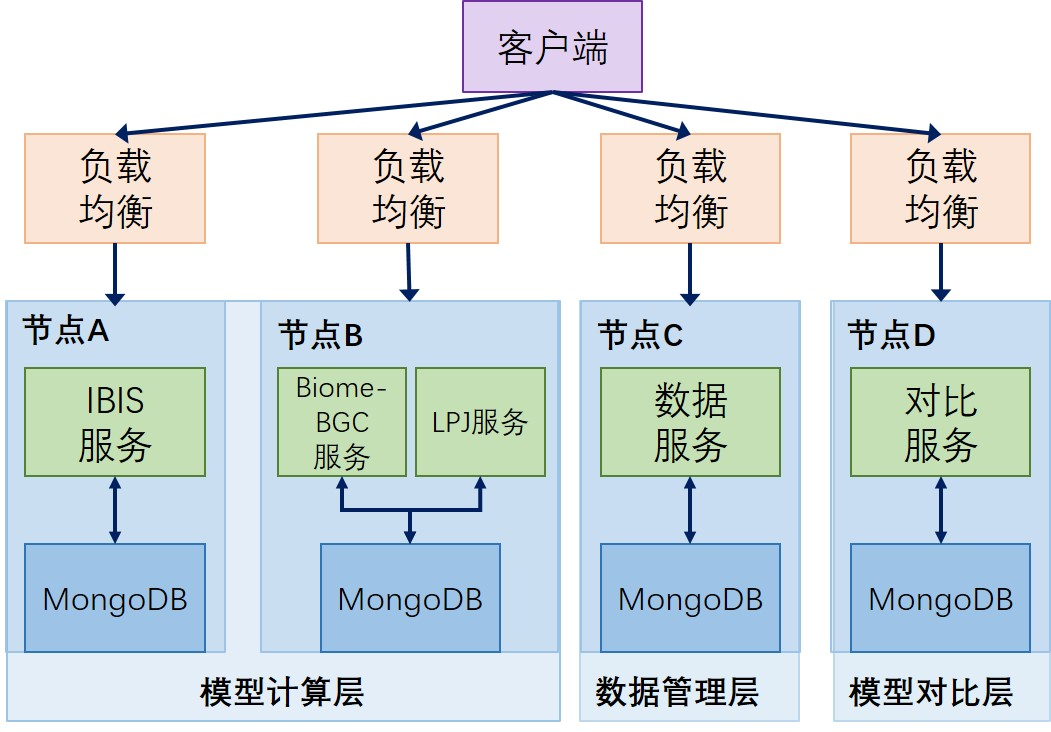
\includegraphics[width=0.6\textwidth]{multi-arch}}
    \hfill
    \subcaptionbox{单体服务应用架构\label{single-arch}}{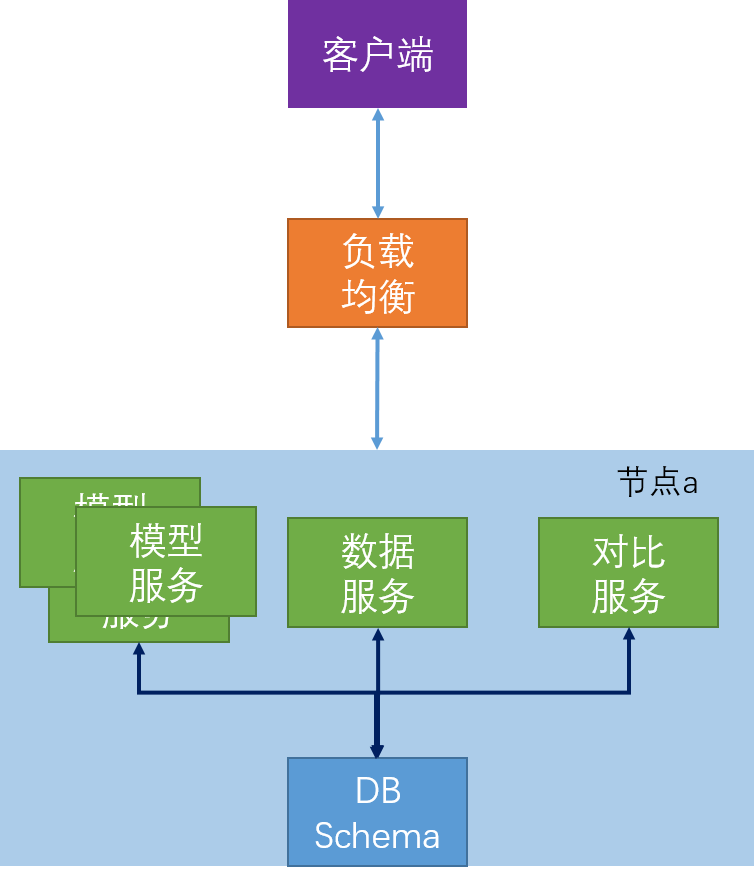
\includegraphics[width=0.35\textwidth]{single-arch}}

    \caption{微服务架构与单体服务架构的对比}
    \label{fig:ms-server-microservice}
\end{figure}

如图~\ref{fig:AKF-cube}所示,微服务的特点可以用AKF立方体~\cite{abbott2009art}表示,应用程序的开发可以抽象为三个维度:

\begin{enumerate}[(1)]
    \item \textbf{X轴:}水平复制。将单体系统运行多个实例,并在其间做负载均衡;
    \item \textbf{Y轴:}功能拆分。基于不同的业务将功能划分为不同的微服务;
    \item \textbf{Z轴:}数据分区。对应用程序的数据库进行拆分,避免遇到数据库瓶颈。
\end{enumerate}

理论上按照这三个维度的扩展模式,可以将单体系统进行无限扩展。

如图~\ref{micro-arch}所示,本文将整个对比工作分为模型计算、数据存储和模型对比三大部分,每一部分划分为微服务实现,其中模型微服务根据模型的软硬件需求,可以将多个模型部署在同一台计算机上,也可以单独部署,由于IBIS模型计算较慢,对软硬件需求较高,本文把他独立部署在一台节点上,而Biome-BGC和LPJ相对来说计算很快,将他们部署在一起。
图~\ref{single-arch}展示了传统的单体服务架构,它将所有功能需求都放在同一台服务器上实现,使得系统庞大臃肿,而与之相比微服务效率高、灵活性强、可用性高、可扩展性强。
% \begin{figure}[!htbp]
%     \centering
%     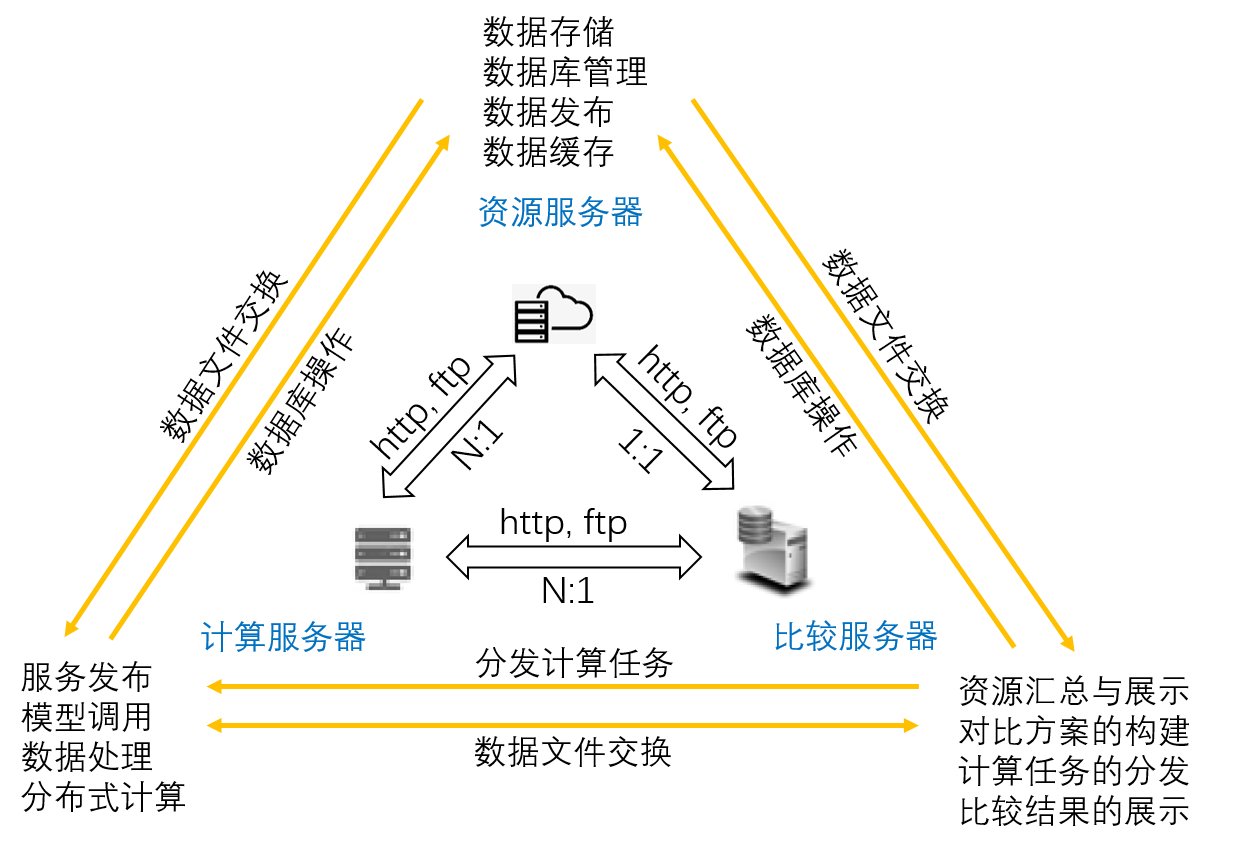
\includegraphics[width=1\textwidth]{network-archecture}
%     \caption{分布式网络架构}
%     \label{fig:network-archecture}
% \end{figure}

\subsection{服务治理}
微服务通过功能分解为系统带来无限扩展的可能,通过功能分解带来优点的同时在集成时也面临着一系列的问题,比如如何发现服务?如何统一对服务进行认证管理?如何针对对比需求进行服务集成?这些都是需要解决的问题。
\subsubsection{服务注册与发现}
传统的单体应用之间耦合关系较少,往往通过手动配置IP地址和端口,但是在微服务架构下,服务提供者会不断扩展而变得越来越多,手动配置的方式并不适用于此,而是通过服务注册来解决。本文设计的注册分两个层级,如图~\ref{fig:service-registe-discover}所示,第一级是在计算节点内部的注册,由计算节点自己独立管理,比如模型计算节点可以发布一个模型服务,也可以发布多个模型服务;第二级是将计算节点注册到中心服务器的数据库中,在计算节点启动时,自动向中心服务节点发送连接请求,并持续发送心跳,当计算节点宕机或手动注销时,心跳停止,中心服务器能够实时更新出注册的节点列表。

\begin{figure}[!htbp]
    \centering
    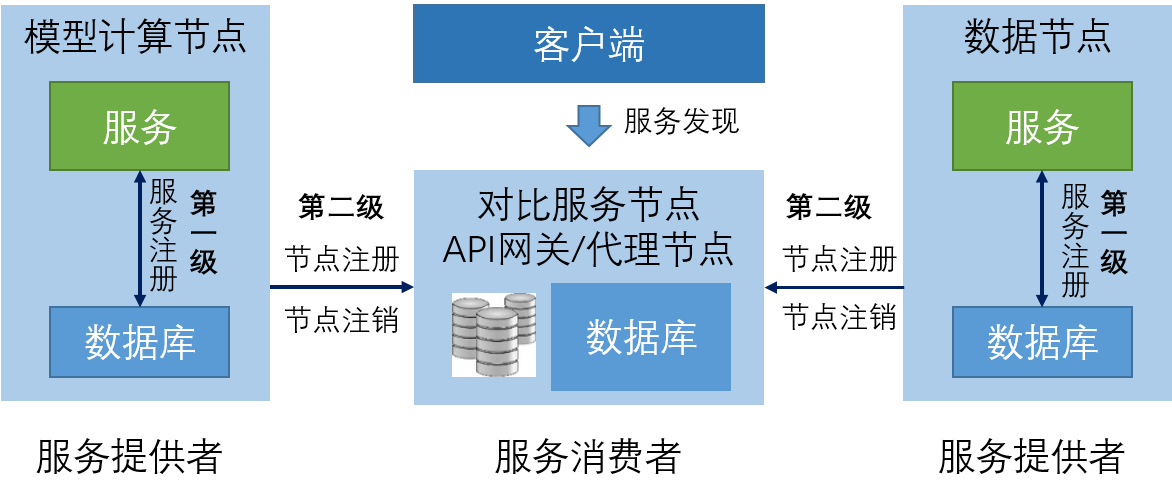
\includegraphics[width=.9\textwidth]{service-registe-discover}
    \caption{服务注册与发现}
    \label{fig:service-registe-discover}
\end{figure}

\subsubsection{API网关}
API网关也是针对微服务而出现的技术手段,在单体应用中,客户端需要请求的后台服务器只有一台,而微服务架构下,需要连接的后台节点就多种多样了,他们往往具有异构的接口、协议,以及许多重复化的功能单元(如认证),这大大增加了客户端逻辑的复杂度。如图~\ref{fig:API-gateway},API网关的设计则是在这些服务节点之上做出一次代理或简单处理,从而屏蔽微服务之间的异构性,使客户端感觉不到微服务的存在。此外,不同的微服务可以通过API网关共同管理其会话状态,从而达到状态共享的目的。在本系统中,API网关和模型对比服务器是同一个实体,在模型对比服务器上,对模型计算服务、数据服务进行服务集成,并做出负载均衡优化。

\begin{figure}[!htbp]
    \centering
    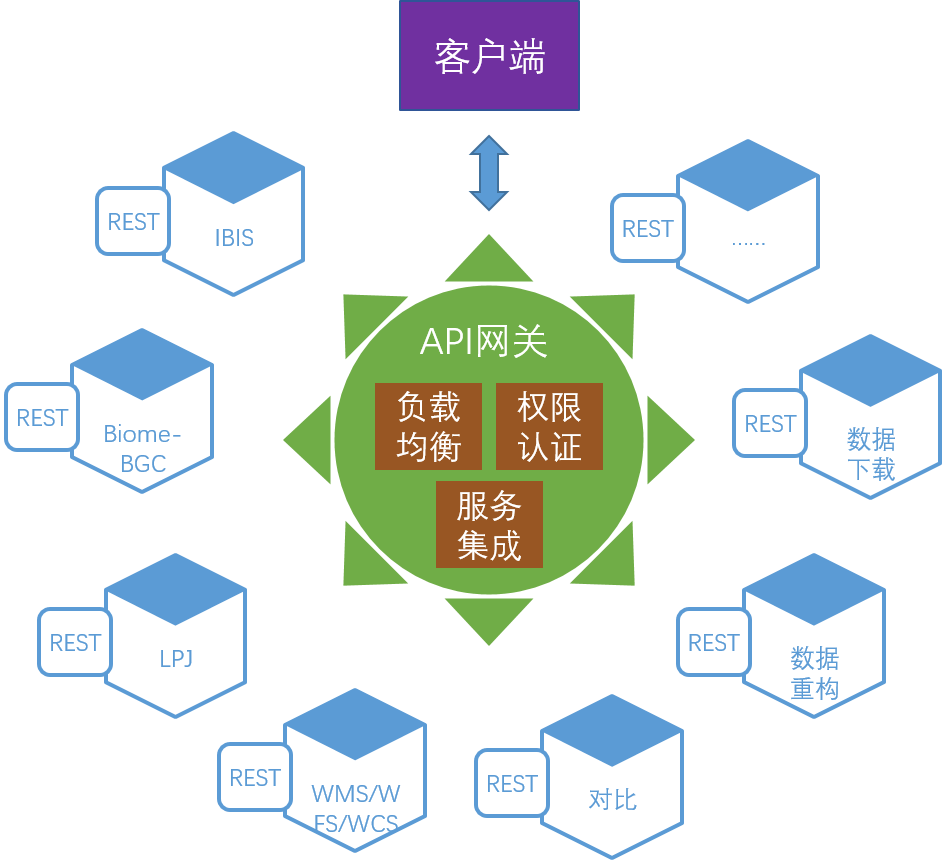
\includegraphics[width=.65\textwidth]{API-gateway}
    \caption{API网关}
    \label{fig:API-gateway}
\end{figure}

\subsection{微服务容器设计}
根据微服务的划分,每一类微服务都需要服务容器的支撑,按照服务容器类型将网络节点分为三层:数据管理层、模型计算层和模型对比层。数据管理层负责数据相关操作,包括数据存储、数据库管理、数据服务的发布和结果数据的缓存;模型计算层负责模型服务的发布、注册、管理和调用;模型对比层作为门户网站的后台服务器,负责资源的汇总与展示、对比话题和方案的创建、计算任务的分发和对比结果的展示。其中计算服务器对外提供模型微服务,资源服务器对外提供数据微服务,三者通过资源交换和消息通信完成协同完成对比任务。
\subsubsection{数据管理层}
% 功能、特点、服务
数据服务容器主要有以下两点功能:
\begin{enumerate}[(1)]
\item \textbf{数据文件存储和缓存:}数据文件包括各种输入数据、对比参照数据和输出数据。模型在运行时从资源服务器请求输入数据,运行结束后将输出数据存储到资源服务器。对比任务执行时从资源服务器请求模型输出数据和对比参考数据,并将对比结果的图表存储到数据服务容器;
\item \textbf{数据服务的发布:}包括WMS、WFS、WCS、下载服务、上传服务、数据重构服务具体参考第~\ref{sec:data-service}节。
\end{enumerate}

资源服务器的硬件配置要求是硬盘大,网络带宽高,以方便数据存储和交换。

% \begin{figure}[!htbp]
%     \centering
%     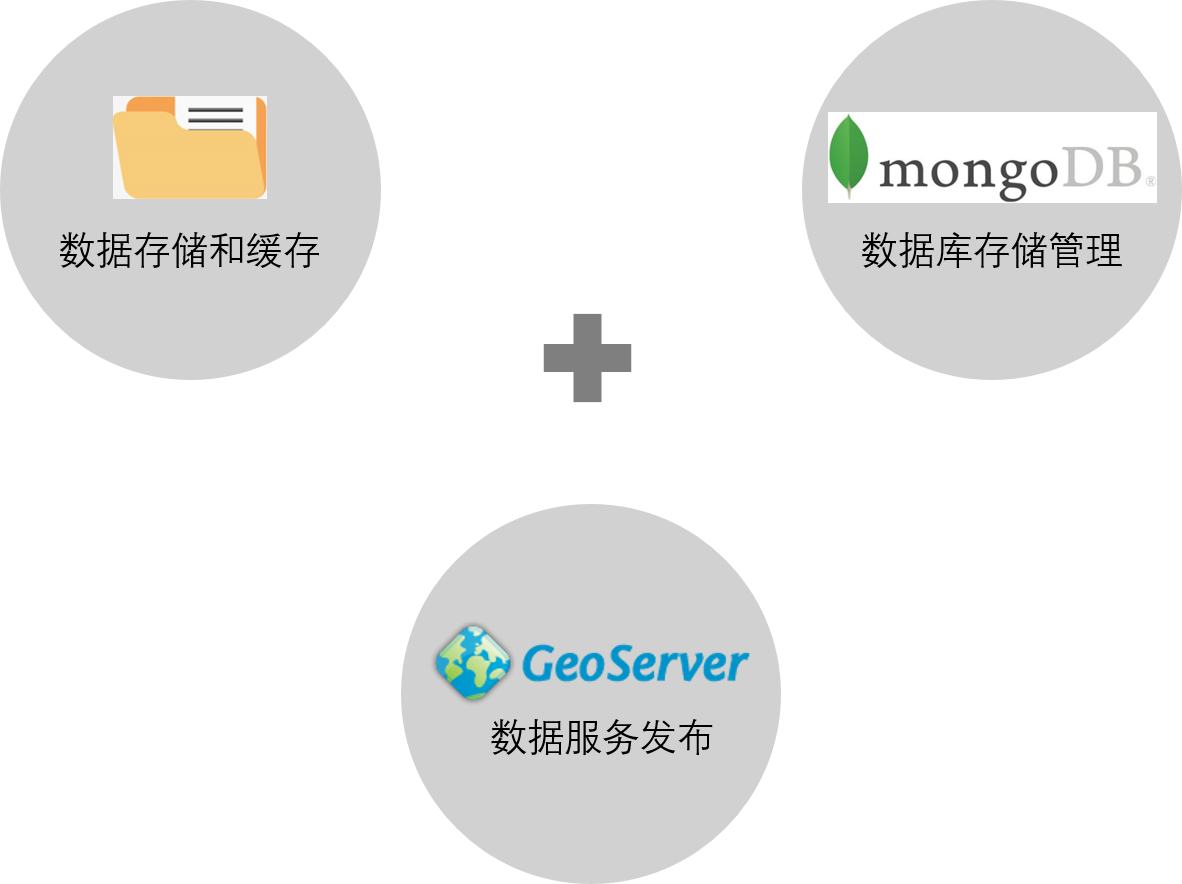
\includegraphics[width=1\textwidth]{resource-server}
%     \caption{资源服务器功能}
%     \label{fig:resource-server}
% \end{figure}

% \begin{figure}[!htbp]
%     \centering
%     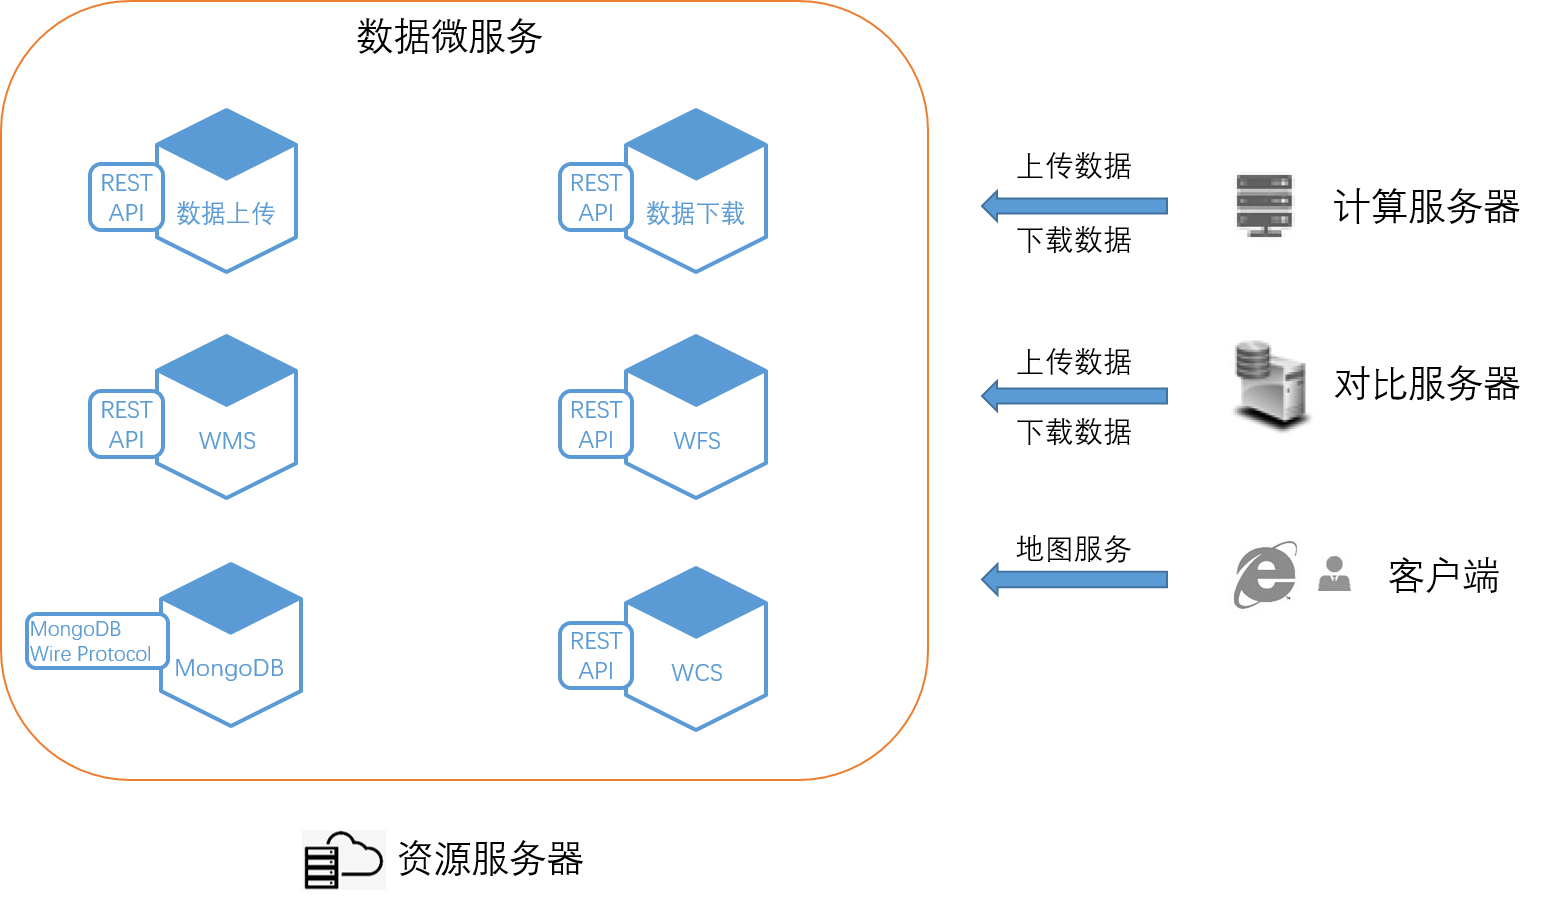
\includegraphics[width=1\textwidth]{resource-server-microservice}
%     \caption{资源服务器微服务}
%     \label{fig:resource-server-microservice}
% \end{figure}


\subsubsection{模型计算层}
\begin{figure}[!htbp]
    \centering
    \subcaptionbox{模型微服务的发布和调用}{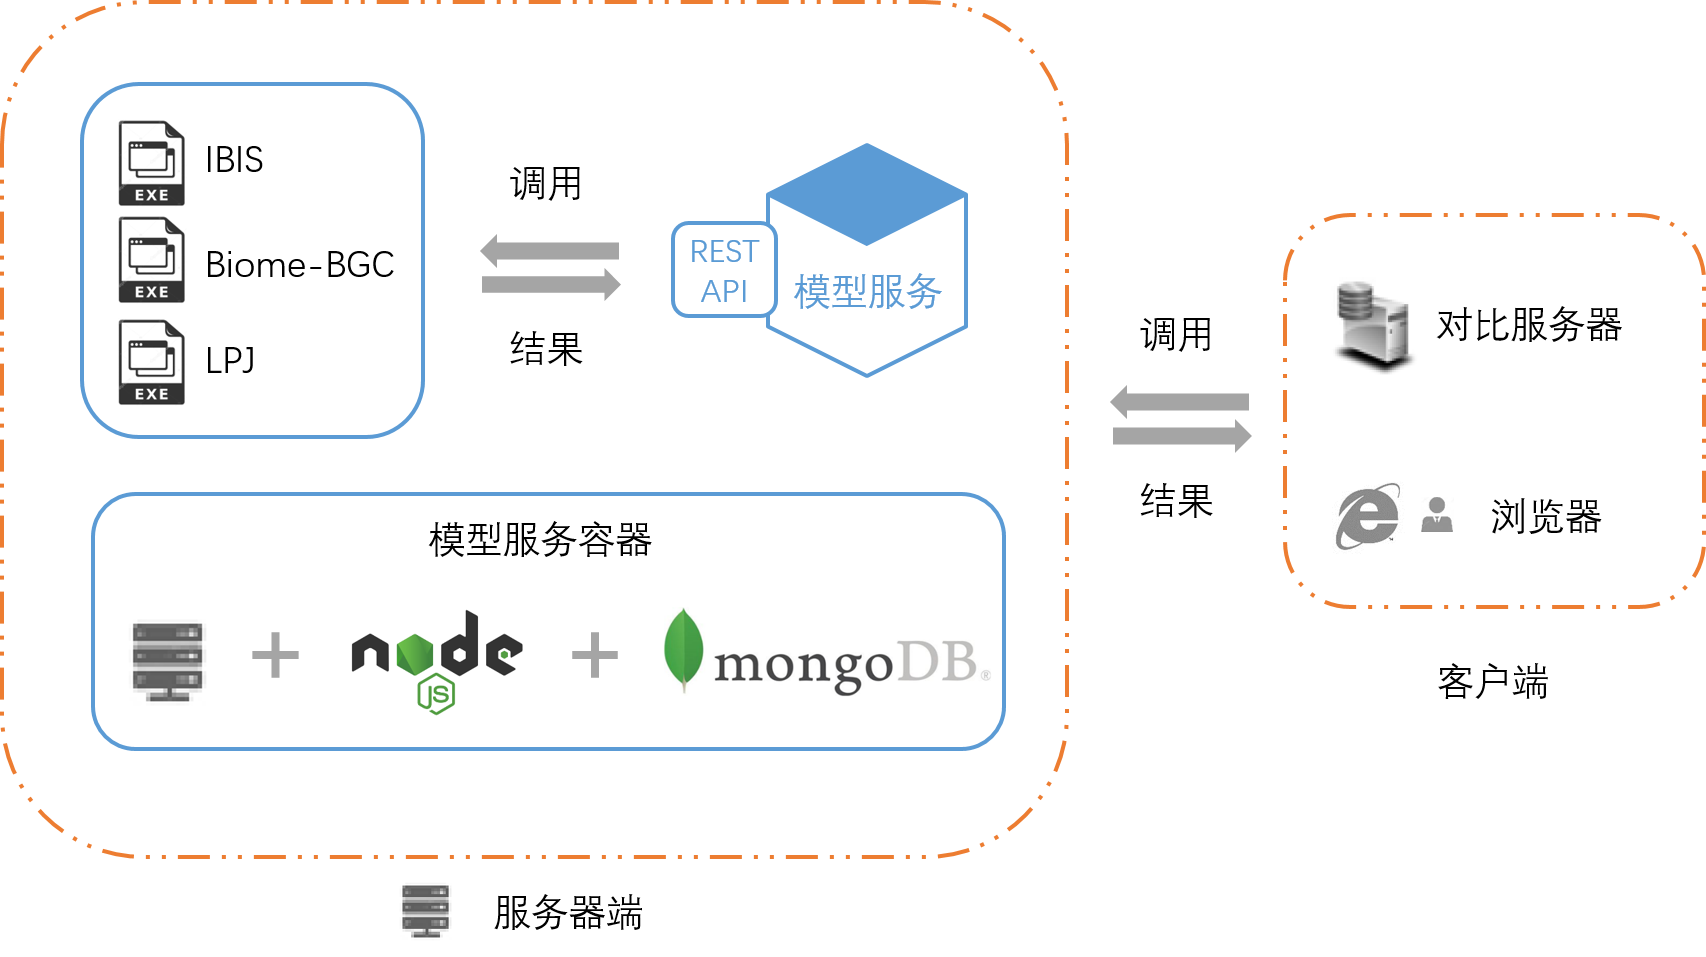
\includegraphics[width=0.65\textwidth]{ms-server-microservice-a}}
    \hfill
    \subcaptionbox{模型微服务多节点分布}{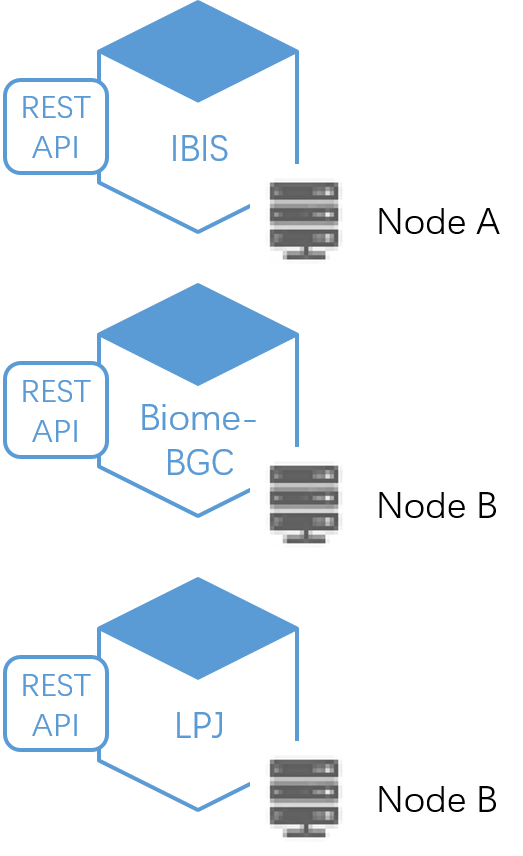
\includegraphics[width=0.25\textwidth]{ms-server-microservice-multi-nodes}}
    \caption{计算服务器微服务}
    \label{fig:ms-server-microservice}
\end{figure}

计算服务容器的主要功能是模型服务的发布、注册、管理和调用,如图~\ref{fig:ms-server-microservice}所示,计算服务容器由Node.js和MongoDB开发。Node.js对外暴露模型调用的接口,当客户端经过HTTP协议发送调用请求时,在计算服务容器内部调用模型应用程序。当模型运行结束后,计算服务容器获取子程序的句柄,将运行结果的状态保存到MongoDB中。模型微服务与数据微服务有一些不同之处:每个独立的模型服务可以根据软硬件需求存放在不同的服务器上,即模型微服务有多计算节点的特性。因此,模型微服务发布后,还需要将服务注册到模型服务资源库中,从而能够被服务消费者发现服务。

\subsubsection{模型对比层}
对比服务容器的主要功能是将对比任务中包含的计算任务分发给计算服务容器,并把模型计算出来的结果文件和对比参考数据进行对比。他是模型微服务和数据微服务的消费者、对比微服务的生产者。如图~\ref{fig:compare-server-microservice}所示,模型对比的开展主要包括以下几步:

\begin{enumerate}[(1)]
\item 用户在浏览器客户端通过HTTP协议发送对比任务的调用请求;
\item Node.js的路由器收到请求后,将对比任务中包含的计算任务拆分出来,并通过调用计算服务器上的模型微服务启动计算任务,并不断轮询监控模型的运行进度;
\item 当监测到所有模型都运行成功后,从资源服务器上发布的模型运行结果微服务和对比参考数据微服务下载数据,然后调用本地的对比方法脚本程序,这些脚本可由JavaScript、Python或Matlab等编写而成;
\item 最后将对比脚本的结果文件保存到数据库中,并返回给客户端。
\end{enumerate}

另外他作为门户网站的后台服务器,还负责浏览器前台的一系列操作,如资源汇总与展示、对比流程的创建、对比结果的展示等。

\begin{figure}[!htbp]
    \centering
    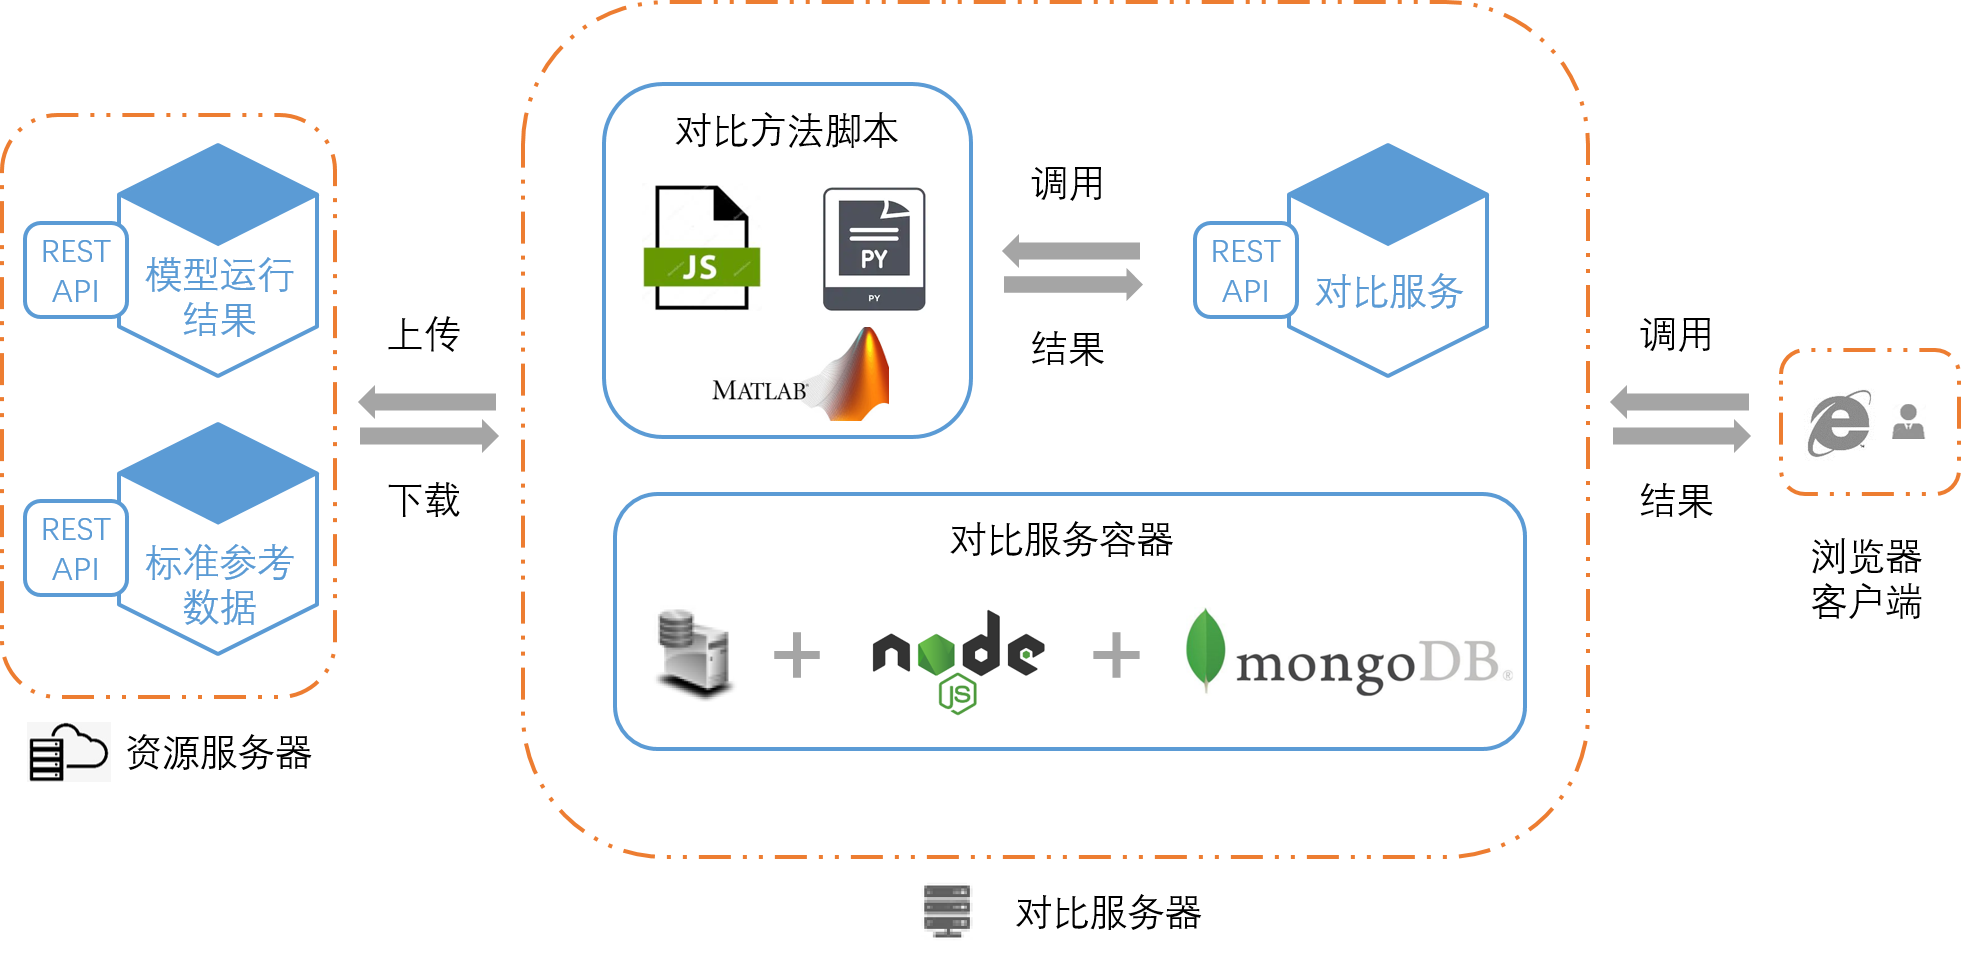
\includegraphics[width=1\textwidth]{compare-server-microservice}
    \caption{对比服务器微服务}
    \label{fig:compare-server-microservice}
\end{figure}

\section{对比科学工作流引擎}
% % 模型调用-数据缓存-数据重构-数据对比
% 微服务是基础设施

\subsection{对比流程分析和归纳}
图~\ref{fig:workflow-example}展示了传统方法在本地进行对比时的流程,整个流程可以概括为“模型计算——数据重构——结果对比”三步。模型计算过程中对比参与者同时输入数据启动运行;数据重构过程将运算结果转换为标准化数据;结果对比过程使用脚本分析。当加入新的对比参与者时整个对比流程也不会发生变化。

\begin{figure}[!htbp]
    \centering
    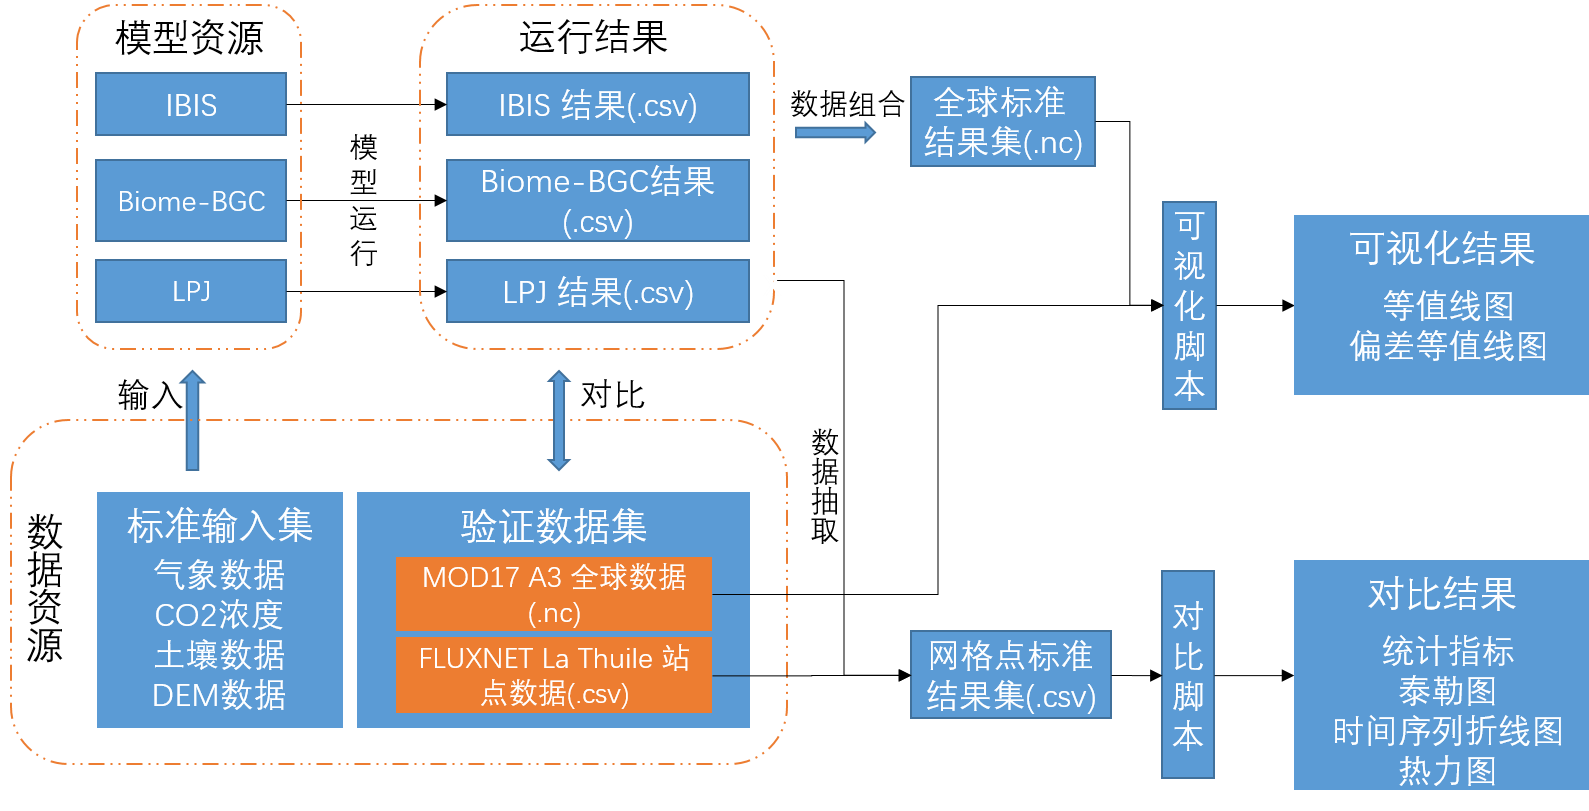
\includegraphics[width=1\textwidth]{workflow-example}
    \caption{以IBIS、Biome-BGC、LPJ三个模型为例的对比流程}
    \label{fig:workflow-example}
\end{figure}

\subsection{对比自动化执行引擎}
%  流程创建:是对工作流过程的抽象表示,定义工作流执行时使用的资源,其依赖关系着重表达了各任务之间从数据生产者到数据消费者的流程,这些资源是指可执行网络服务、数据,对应对比方案
%  通过流程映射形成可执行的工作流实例,对应对比任务
% 工作流定义:工作流语言通常用XML这种形式化描述语言,表达组成流程的任务和任务之间的依赖关系,SWF没有标准语言,流程定义只能由各自的流程引擎解析执行
% 工作流执行:运行时建立网络资源之间的交互关系,将抽象工作流转换成可执行的工作流,建立任务和所需可用资源的映射关系
% 工作流活动之间的依赖主要表达了多个任务之间的逻辑结构和执行方式,包括顺序、并行、循环、条件
在微服务架构下,面临着服务集成的问题,科学工作流是服务集成的一个解决方案。 % 具体化,数据传输的流程
工作流管理联盟(Workflow Management Coalition,WfMC)将工作流定义为一类能够完全或者部分自动执行的经营过程,根据一系列过程规则,文档、信息、或任务能够在不同的执行者之间传递、执行。科学工作流是工作流的一种,它主要面向科学实验过程,以数据驱动,用来描述和控制科学实验和过程的执行~\cite{ludascher2006scientific}~\cite{Zhao2009Special}。

科学工作流的生命周期可归纳为一下三点:
\begin{enumerate}[(1)]
    \item \textbf{流程创建:}定义工作流执行时所参与的活动,以及数据在活动之间的流向关系,在本文中活动是指各种模型服务、数据重构服务和对比服务。定义出的工作流表达了数据从生产者到消费者之间的流向关系,但还不包括数据实体;
    \item \textbf{流程映射:}绑定活动所需要的数据实体,从而将工作流映射为可执行的工作流实例;
    \item \textbf{流程执行:}解析工作流中活动的依赖关系,并在网络环境下进行运算。
\end{enumerate}

在本文的对比流程中,工作流模式固定,如图~\ref{fig:workflow},都是分“模型计算——数据重构——模型对比”三步,所以不再通过图形化界面创建工作流,只需要通过选择对比参与者和对比方法就能够重现出这三流程,所以本文的工作流可以通过对比方案表达,流程创建对应对比方案的创建,流程映射对应对比任务的创建,流程执行对应对比任务的执行。

% 每一步都是在网络环境下,有频繁的数据传输交互

\begin{figure}[!htbp]
    \centering
    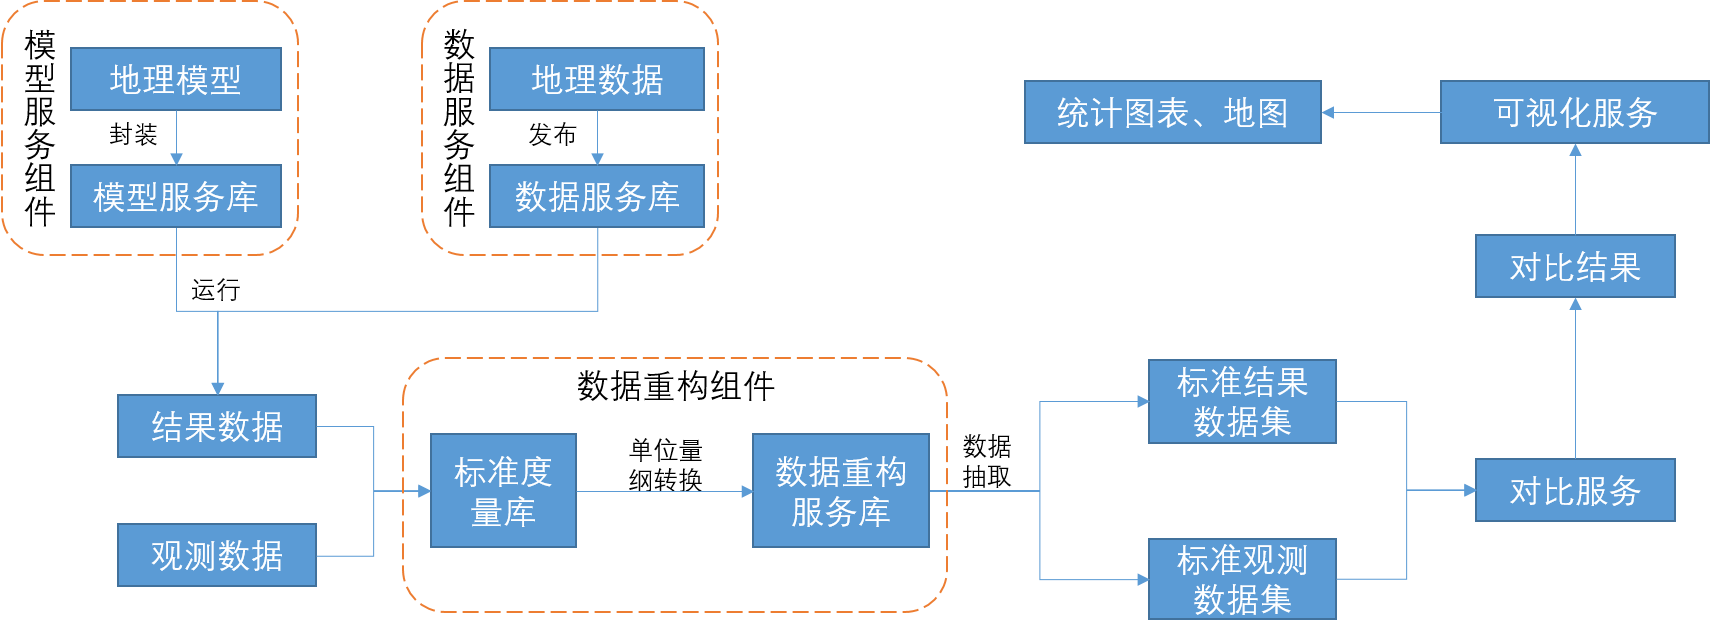
\includegraphics[width=.5\textwidth]{workflow}
    \caption{开放式对比科学工作流流程图}
    \label{fig:workflow}
\end{figure}

\section{本章小结}
开放式对比系统的构建有两个关键问题:一是如何设计一个开放式的对比框架,二是这些对比资源如何接入框架。对于问题一,本章从对比业务、资源组件、网络架构和执行引擎四个角度进行了详细论述,设计的系统框架具有以下特点的:

\begin{enumerate}[(a)]
    \item 模型计算和对比可共享与重用;
    \item 模型计算和对比过程公开化;
    \item 模型和数据资源可扩展性地动态接入;
    \item 大规模计算场景下稳定可用;
    \item 以自动化实现其易用性。
\end{enumerate} 

对于问题二将在下一章详细论述。
\chapter{开放式对比资源接入方法}
本文将数据、模型和对比方法称之为对比资源,这三者的开放性决定了对比结果的准确性、公开性和公平性。其中模型作为对比的对象,是本系统中最重要的要素之一。传统的模型对比方案将模型部署在本地环境运行,针对第\ref{sec:cmp-sln-analysis}节分析的多对比情景需求,会造成难以共享和重现等问题,本章描述的模型服务化封装、部署和发布对此提出了对策;而数据资源作为支撑模型成功运行的必备要素,传统的基于数据拷贝的方式在这种情景下也不能满足要求,因此本章对数据资源的开放式接入也提出了相应的方案;在这两者的基础之上,将统计学对比方法和可视化对比方法也通过服务封装发布,实现了对比资源的统一开放式接入。

\section{开放式碳循环数据资源接入方法}
\label{sec:data-joinup}
网络空间中的数据按照其组织结构可以分为结构化数据、半结构化数据和非结构化数据,地理模型在运行时强烈依赖于输入数据的结构,所以半结构化和非结构化数据的结构化描述是数据应用时重要部分。
本节首先从数据格式、尺度、编排三个方面详细地分析了碳循环相关数据资源的特征,对领域通用数据设计了结构化的描述接口,以帮助数据资源介绍、接入、匹配和展示。最后遵循OGC WMS、WFS、WCS标准,使用GeoServer发布碳循环数据服务,实现了空间数据的在线预览和查询检索,对于对比过程中需要进行的数据抽取和重组,设计了数据重构服务以解决数据与模型难以适配的适配问题。

\subsection{碳循环数据资源结构特征分析}
\subsubsection{数据格式分析}
碳循环相关数据主要有几种格式:NetCDF、CSV、Shapefile和TXT,如表~\ref{tab:data-format-feature}所示,这些数据都是非结构化的。

\begin{table}[H]
    \centering
    \caption{数据格式和特征}
    \label{tab:data-format-feature}
    \begin{threeparttable}
        \begin{tabular}{lll|l}
            \Xhline{1.5pt}
            数据格式 & 数据类型 & 维数 & 数据名称 \\
            \Xhline{1.5pt}
            \multirow{2}{*}{Shapefile} & \multirow{2}{*}{矢量数据} & \multirow{2}{*}{2维} & 网格点 \\
            \cline{4-4}
            & & & 观测站点 \\
            \hline
            \multirow{5}{*}{NetCDF} & \multirow{5}{*}{场数据} & \multirow{5}{*}{n维} & DEM \\
            \cline{4-4}
            & & & MERRA 2 \\
            \cline{4-4}
            & & & Soil \\
            \cline{4-4}
            & & & PFT \\
            \cline{4-4}
            & & & 全球计算结果 \\
            \hline
            \multirow{2}{*}{\makecell{CSV}} & \multirow{2}{*}{二维表} & \multirow{2}{*}{2维} & 网格点输入气象数据 \\
            \cline{4-4}
            & & & 网格点计算结果 \\
            \hline
            \multirow{3}{*}{\makecell{TXT}} & \multirow{3}{*}{文本数据} & \multirow{3}{*}{1维} & $CO_2$浓度 \\
            \cline{4-4}
            & & & PFT \\
            \cline{4-4}
            & & & Biome-BGC的运行配置 \\
            \Xhline{1.5pt}
        \end{tabular}
    \end{threeparttable}
\end{table}

\begin{enumerate}[(1)]
    \item \textbf{NetCDF}
    
    NetCDF(network Common Data Form)网络通用数据格式是由美国大学大气研究协会的Unidata项目科学家针对科学数据的特点开发的,是一种面向数组型并适于网络共享的数据的描述和编码标准,已被作为OGC的一项标准使用。NetCDF数据通常用来表示多维场数据,从数学上来看,它存储的数据就是一个多自变量的单值函数:$f(x,y,z,...)=value$。其中$x,y,z$等在NetCDF中被称为维(Dimension),函数值$value$被称为变量(Variables),维和变量在物理学上的一些性质,被称为属性(Attributes)。当维度只有经纬度时,可以用来表示栅格数据,如本文中的植被功能类型数据、DEM数据、土壤质地数据。维度除了经纬度以外通常还有时间维,如本文中的MERRA 2气象数据和全球范围内的模型计算结果。具体的维度和变量信息如表~\ref{tab:nc-dim-var} % 参考百度百科

    \begin{table}[H]
        \centering
        \caption{NetCDF数据的维度和变量列表}
        \label{tab:nc-dim-var}
        \begin{threeparttable}
            \begin{tabular}{lll}
                \Xhline{1.5pt}
                数据名称 & 维度 & 变量 \\
                \Xhline{1.5pt}
                DEM & 经度、纬度 & 高程 \\
                \hline
                MERRA 2 & 经度、纬度、时间 & \multicolumn{1}{m{0.4\columnwidth}}{最低温、最高温、平均温、相对湿度、降水、风速、云量} \\
                \hline
                Soil & 经度、纬度 & \multicolumn{1}{m{0.4\columnwidth}}{沙粒含量、黏粒含量、粉粒含量} \\
                \hline
                PFT & 经度、纬度 & 植被类型编号 \\
                \hline
                全球计算结果 & 经度、纬度、时间 & \multicolumn{1}{m{0.4\columnwidth}}{GPP、NPP、NEP、Biomass、ET} \\
                \Xhline{1.5pt}
            \end{tabular}
        \end{threeparttable}
    \end{table}

    \item \textbf{CSV}
    
    CSV(Comma-Separated Values)逗号分隔符文件是以文本形式存储的表型数据。CSV文件由任意数量的记录组成,每行称之为一条记录,每条记录由多个字段组成,字段之间由分隔符分割,通常是逗号或制表符。CSV文件有一系列的规则,比如可以选择性的包含列名,开头不能留空行,每条记录不能跨行等。本文中的CSV文件有网格点气象数据、网格点结果数据和站点观测数据,他们除了具备常规CSV文件的特点以外,还都用一列来表示时间。

    \item \textbf{Shapefile}
    
    Shapefile是ESRI开发的一种矢量空间数据格式,也属于OGC的一项标准。Shapefile文件用点线面描述空间对象的几何信息,用属性表描述对象的属性,另外还包括有数据的空间参考坐标、图形索引等。本文中用到的Shapefile数据是由$0.5^{\circ} \times 0.5^{\circ}$的经纬网划分而来的网格点。

    \item \textbf{TXT}
    
    TXT文件是最常用的文件格式,没有固定的结构。

\end{enumerate}

\subsubsection{数据尺度分析}
尺度是地理学数据的重要特征,指数据集表达的时空范围和精度,不同尺度数据表达的信息密度有很大差异。
\begin{enumerate}[(1)]
    \item \textbf{时间尺度}
    
    主要指数据的时间范围和精度,碳循环的数据和模拟有很强的多样性,精度上可细分为日尺度、月尺度、季节尺度、年尺度、百年尺度等,范围上包括1年、多年甚至几十年。本文的模拟全部在日尺度上进行,模拟时间范围为1982年到2014年,观测数据的时间范围视具体站点而定,一般为1-10年左右。在对比时,由于日尺度的时间序列长度比较大,且数据噪点比较多,因此,也需要对其时间分辨率进行调整,以月尺度、季节尺度和年尺度对其进行平滑,可以提高数据的精度。

    \item \textbf{空间尺度}
    
    主要体现在数据的空间范围和分辨率上。如表~\ref{tab:spatial-multi-resulotion}所示,各种输入数据的分辨率和范围不尽相同,本文统一重采样为$0.5^{\circ} \times 0.5^{\circ}$,并以其划分网格在全球范围内模拟。

    \begin{table}[H]
        \centering
        \caption{碳循环模拟的空间多尺度特征}
        \label{tab:spatial-multi-resulotion}
        \begin{threeparttable}
            \begin{tabular}{lrrrr}
                \Xhline{1.5pt}
                数据名称 & 经度分辨率 & 纬度分辨率 & 北纬边界 & 南纬边界 \\
                \Xhline{1.5pt}
                模拟输入和输出 & $0.5^\circ$ & $0.5^\circ$ & $82.25^\circ$ & $-54.75^\circ$ \\
                MERRA 2 & $0.625^\circ$ & $0.5^\circ$ & $90^\circ$ & $-90^\circ$ \\
                DEM & $0.5^\circ$ & $0.5^\circ$ & $89.75^\circ$ & $-89.75^\circ$ \\
                土壤 & $0.0085^\circ$ & $0.0107^\circ$ & $90^\circ$ & $-90^\circ$ \\
                植被功能类型 & $0.66^\circ$ & $0.5^\circ$ & $90^\circ$ & $-90^\circ$ \\
                MODIS 17 A3 GPP/NPP & $0.0083^\circ$ & $0.0083^\circ$ & $80^\circ$ & $-60^\circ$ \\
                \Xhline{1.5pt}
            \end{tabular}
        \end{threeparttable}
    \end{table}

\end{enumerate}

\subsubsection{数据编排分析}
\label{subsubsec:data-arrange}
\begin{figure}[!htbp]
    \centering
    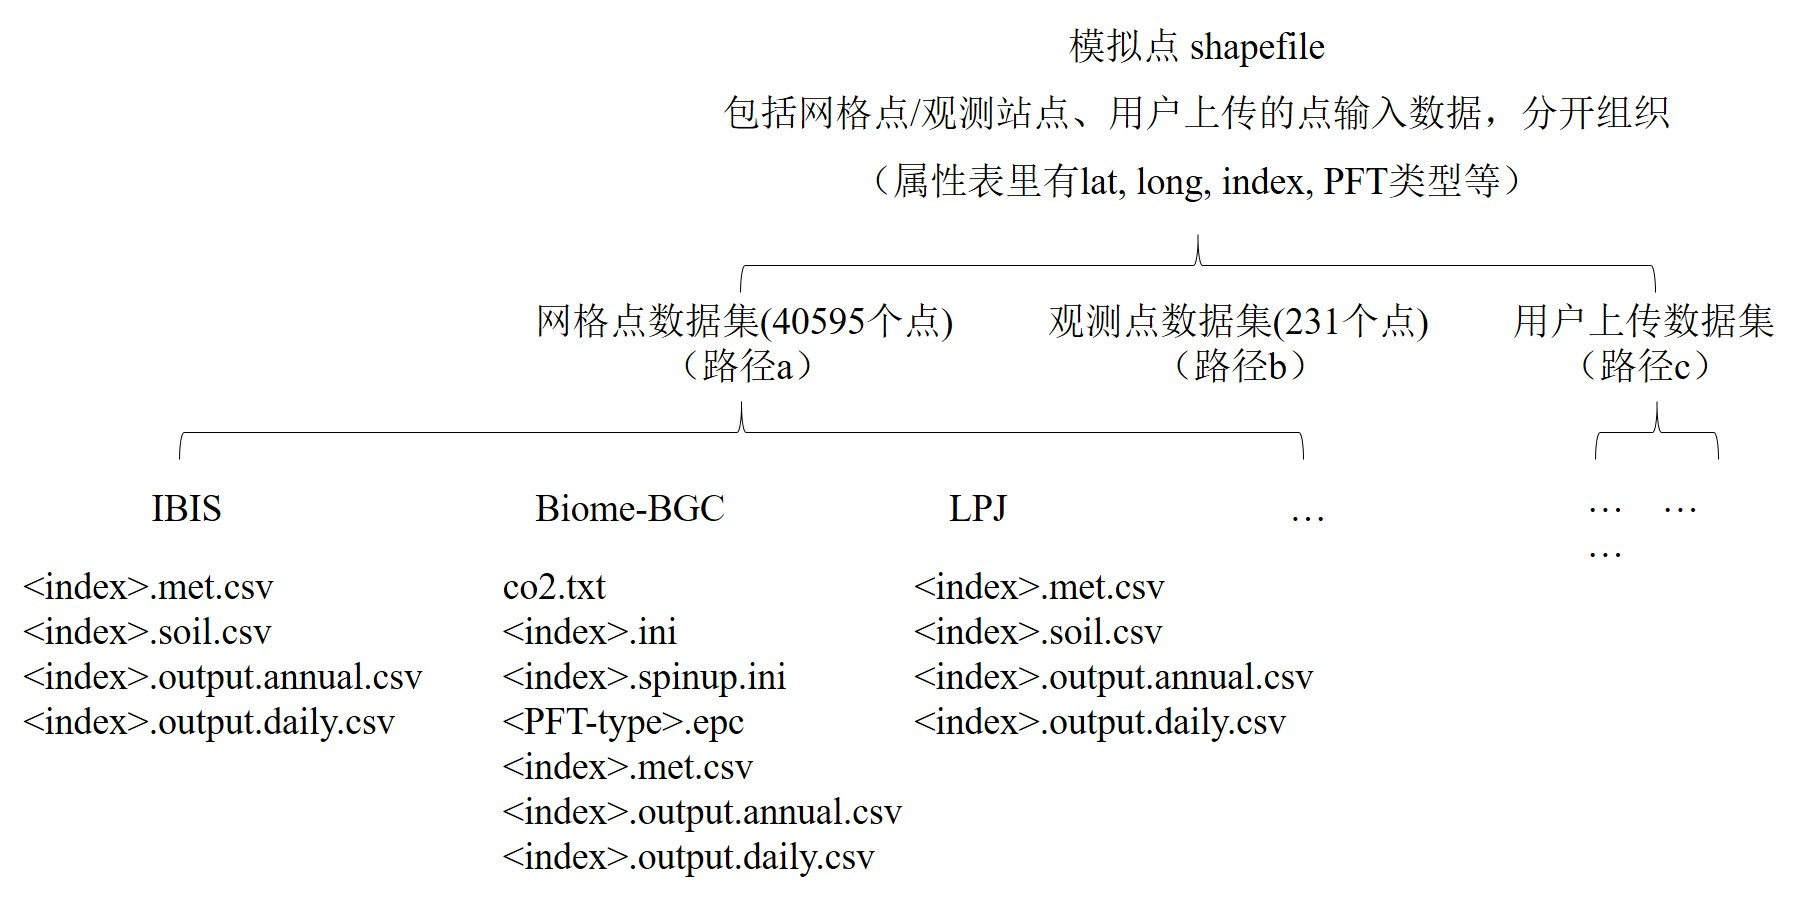
\includegraphics[width=1\textwidth]{data-arrange}
    \caption{陆地生态系统碳循环模型输入数据编排}
    \label{fig:data-arrange}
\end{figure}

由于三个模型对于数据的要求不完全相同,所以合理的数据编排对数据检索、下载、模型运行都是至关重要的。如图~\ref{fig:data-arrange}所示,每套数据集存放在固定的路径下,可由数据库解析到。在运行一个格点时,首先从网格点shapefile的属性表中获取他的编号,再对应到具体的数据集和模型下面,可以获取详细的输入输出文件列表。

\subsection{碳循环数据资源描述方法}
\label{sec:data-desc}
面对海量异构的数据资源,元数据是帮助人们理解数据最常用的方法,它描述了数据的内容、质量、表示方式、空间参照系、管理方式、数据的所有者、数据的提供方式和数据集的其他特征等,为地理信息的管理、维护和共享提供了基础。对于元数据的描述方法,国内外都有很多对应的研究,OGC采用XML Schema(如GOC Simple Feature规范)来描述GML,来支持WPS的运行~\cite{OGC-WPS}。OpenMI(Open Modelling Interface)设计了一套标准接口用于多模型集成耦合时对数据的定义、描述和传递~\cite{MOORE2005279}。乐松山设计的通用数据表达——交换模型(Universal Data Description eXchange Model,UDX),结合数据映射服务和数据重构服务,面向模型集成应用场景可以对数据结构进行结构化、语义化描述~\cite{2016-yuesongshan-phd}。

\begin{figure}[!htbp]
    \centering
    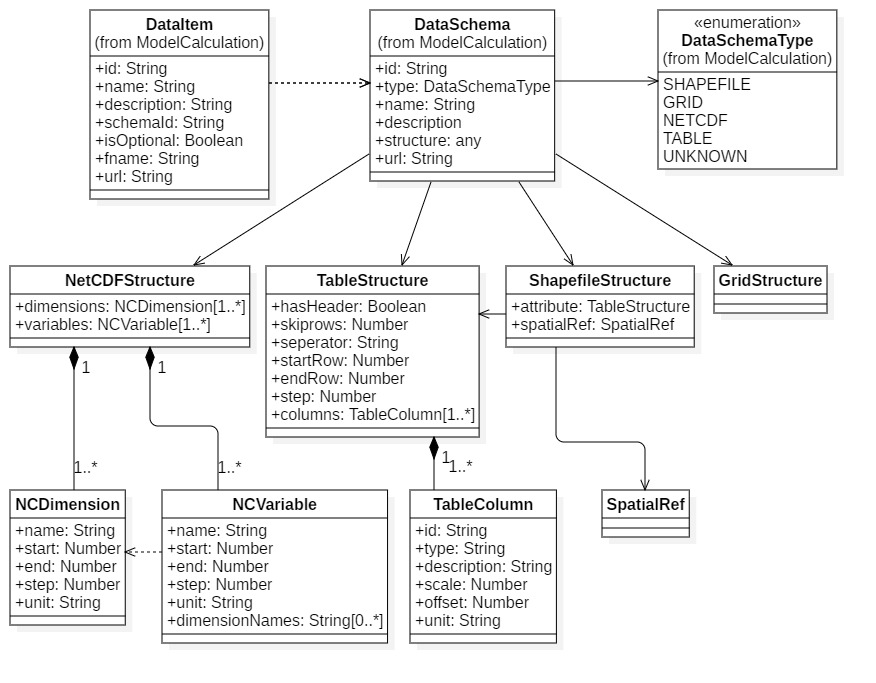
\includegraphics[width=1\textwidth]{jpg/ModelComparison!4-1-data-description-interface_4}
    \caption{数据描述接口设计}
    \label{fig:ModelComparison!4-1-data-description-interface_4}
\end{figure}

为适应本系统的需求,本文并没有采用这些数据描述标准,而是采用自定义结构进行结构化描述。对于数据的描述分为两部分:领域通用格式数据的描述和自定义结构数据的描述。对于后者,本文采用示例数据的形式描述。对于前者,本文设计了如图~\ref{fig:ModelComparison!4-1-data-description-interface_4}所示的数据描述语言(Data Description Language),对领域通用格式数据进行描述:

\begin{enumerate}[(1)]
    \item NetCDF:通过NetCDFStructure结构表达,包括文件的维度(NCDimension)和变量(NCVariable)列表。其中时间、经度、纬度三个维度和变量都使用``unit''、``start''、``end''、``step''表示其数据在时间和空间上的单位、范围和步长。所有变量都使用``scale''、``offset''对数据进行线性变换,使用``missing\_value''描述缺失数据;
    \item CSV:通过TableStructure结构表达,主要用来描述头信息和列信息的解析。针对模型输出结果都包含时间列的特性,本文使用``timeUnit''、``timeStart''、``timeEnd''、``timeStep''描述时间单位、范围和步长。``hasHeader''、``skiprows''、``seperator''用来解析表头,``scale''、``offset''、``unit''用来解析列信息;
    \item Shapefi:通过ShapefileStructure结构表达,其属性表通过指向TableStructure的引用描述,空间参考通过WKT字符串描述。
\end{enumerate}

图~\ref{fig:data-desc-example}展示了CSV和NetCDF格式的数据描述文档示例,对于CSV数据的描述,主要包括解析数据的表头和列信息组成,表头信息包括有无表头、跳过行数、分隔符、起始列号、终止列号、步长信息。列信息包括数据缩放因子、偏移量、描述和单位信息组成。
对于NetCDF数据的描述,包括维度和变量信息。他们都包括名称、缺省值、缩放因子、偏移量等信息。
通过这些时空信息的结构化表达,为数据重构提供了基础支撑。

\begin{figure}[!htbp]
    \centering
    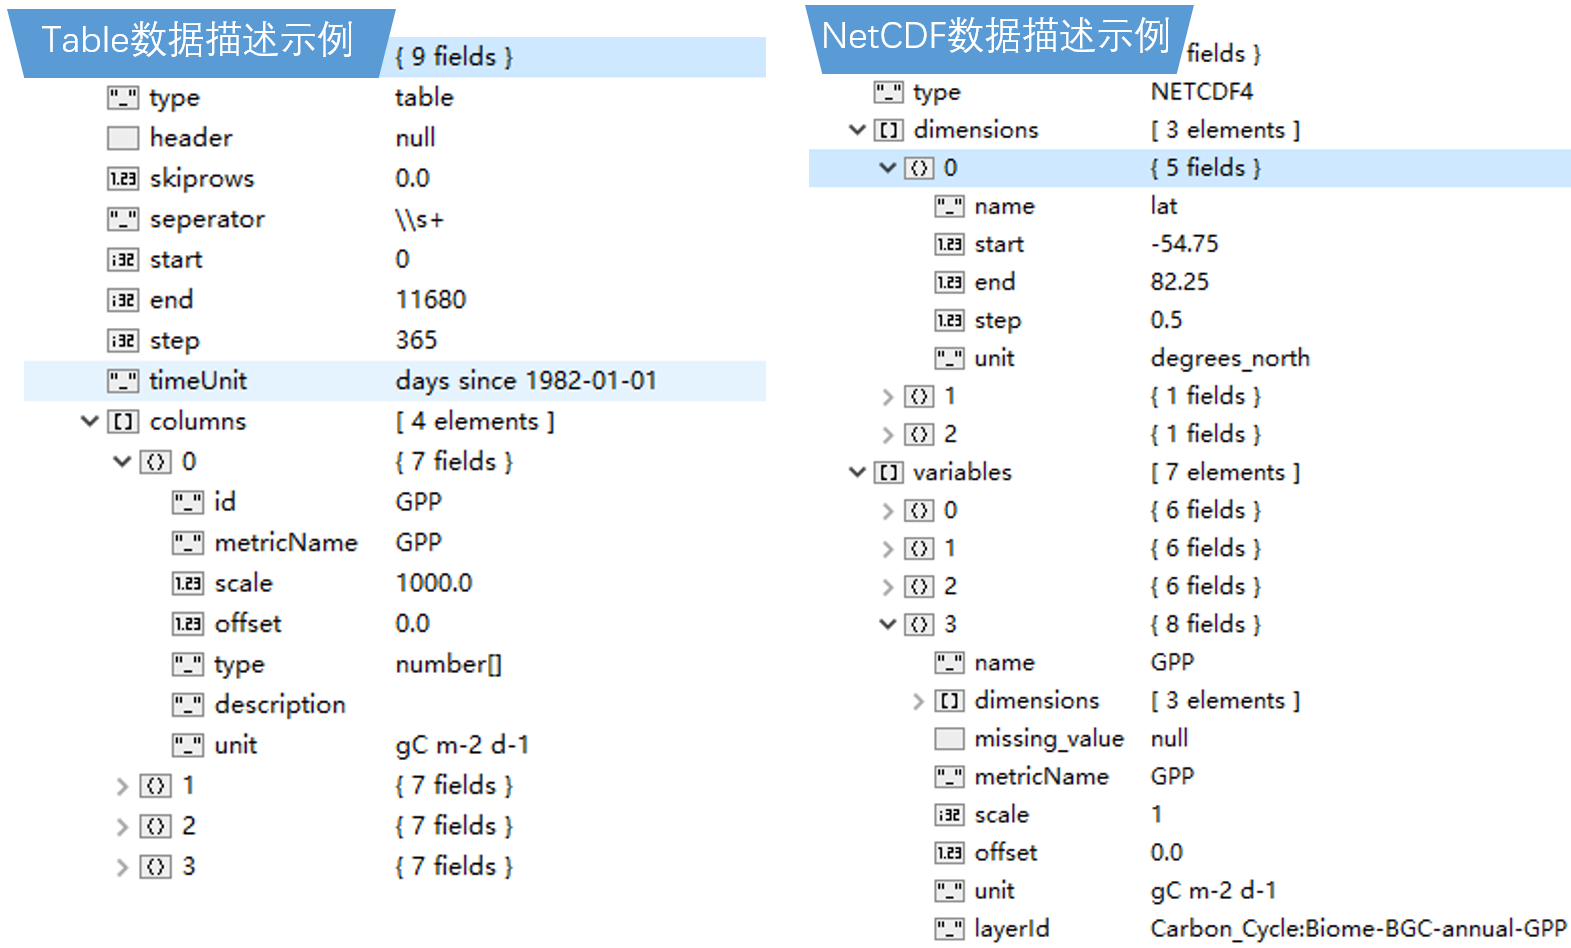
\includegraphics[width=1\textwidth]{data-desc-example}
    \caption{CSV和NetCDF数据描述文档示例}
    \label{fig:data-desc-example}
\end{figure}

\subsection{碳循环数据资源的服务化}
\label{sec:data-service}
\subsubsection{WMS、WFS、WCS三种服务的发布}
\label{subsubsec:OGC}
为实现一套与厂商无关的空间数据互操作规范,开放地理空间信息联盟(OGC)制定了WMS、WFS、WCS服务标准,具体接口如表~\ref{tab:OGC-WMS-WFS-WCS}所示。其中WMS(Web Map Service)利用具有地理空间信息的数据制作地图,在国际规范中,地图是地理数据的可视化表现,WMS返回的地图并非是地图数据,而是地图图像,格式上可以是PNG、GIF、JPEG、SVG等~\cite{OGC-WMS}。WFS(Web Feature Service)通过GML(Geography Markup Language)传递地理空间数据,它支持在基于HTTP协议的分布式计算平台上对地理要素进行增删查改等操作,并在这些操作过程中保证了地理数据变化的一致性~\cite{OGC-WFS}。WCS(Web Coverage Service)在网络上以覆盖(Coverage)的形式共享地理空间数据,能够返回栅格时空范围中任意指定点的值,实现了栅格影像数据集的共享~\cite{OGC-WCS}。

图~\ref{fig:wms-example}是本文发布的WMS图层,图~\ref{fig:wfs-example}是通过WFS查询要素属性的返回结果,图~\ref{fig:wcs-example}是通过WCS下载的全球GPP覆盖的HTTP请求头信息。

\begin{table}
    \centering
    \caption{OGC WMS、WFS、WCS接口}
    \label{tab:OGC-WMS-WFS-WCS}
    \begin{threeparttable}
%        \begin{tabular}{ l | l p{0.5\columnwidth}} 
        \begin{tabular}{ l | l l}
            \Xhline{1.5pt}
            类型 & 接口 & 描述 \\
            \Xhline{1.5pt}
            \multirow{3}{*}{WMS} & GetCapabilities & \multicolumn{1}{m{0.6\columnwidth}}{返回服务级元数据,包括对服务信息内容和可接受请求参数的描述} \\
            \cline{2-3}
            & GetMap & 返回一幅地图影像 \\
            \cline{2-3}
            & GetFeatureInfo & 返回地图上要素的空间实体信息 \\
            \hline
            \multirow{5}{*}{WFS} & GetCapabilities & 返回服务级元数据 \\
            \cline{2-3}
            & DescribeFeatureType & 返回表示要素结构的XML文档 \\
            \cline{2-3}
            & GetFeature & 返回GML形式的要素实例 \\
            \cline{2-3}
            & Transaction & 增删查改事务请求 \\
            \cline{2-3}
            & LockFeature & 在事务期间对一个或多个要素实例上锁 \\
            \hline
            \multirow{3}{*}{WCS} & GetCapabilities & 返回描述服务和数据集的XML文档 \\
            \cline{2-3}
            & DescribeCoverage & 返回对覆盖的详细描述 \\
            \cline{2-3}
            & GetCoverage & 使用覆盖格式(图片)返回地理位置的值或属性 \\
            \Xhline{1.5pt}
        \end{tabular}
        \begin{tablenotes}
            \footnotesize
            \item 详细接口参考OGC~\cite{OGC-WMS}~\cite{OGC-WFS}~\cite{OGC-WCS}。
        \end{tablenotes}
    \end{threeparttable}
\end{table}



\begin{figure}[!htbp]
    \centering

    \subcaptionbox{WMS图层列表\label{wms-layers}}{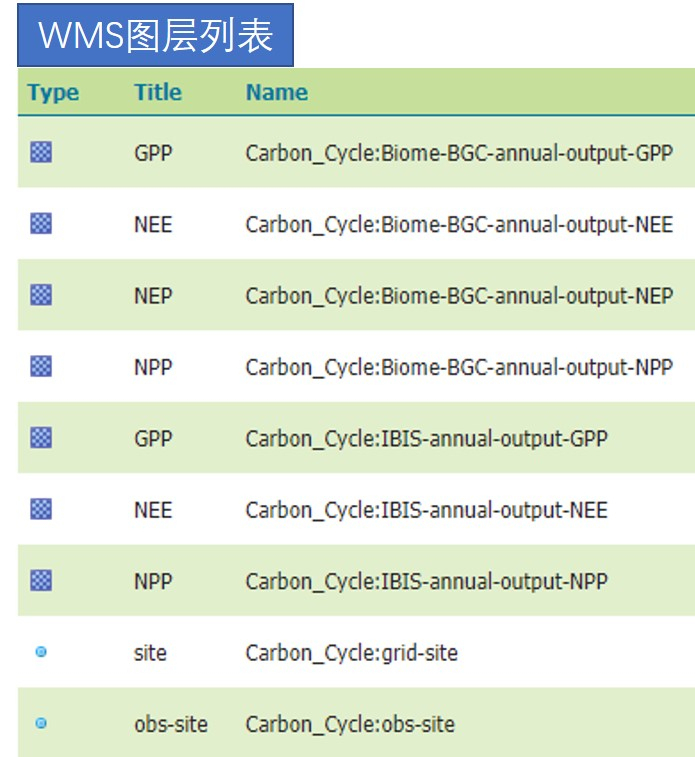
\includegraphics[width=0.35\textwidth]{wms-layers}}
    \hfill
    \subcaptionbox{WMS图层预览\label{wms-example}}{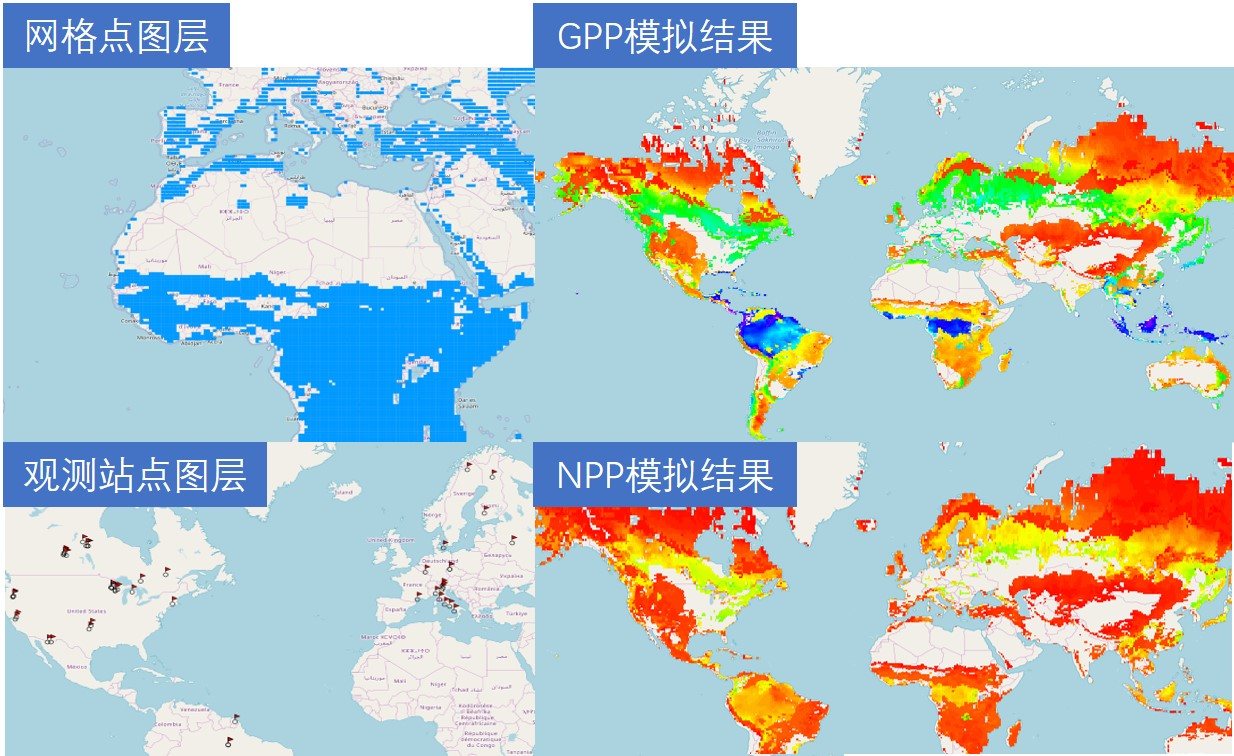
\includegraphics[width=0.6\textwidth]{wms-example}}

    \caption{WMS请求}
    \label{fig:wms-example}
\end{figure}

\begin{figure}[!htbp]
    \centering

    \subcaptionbox{WFS请求\label{fig:wfs-example}}{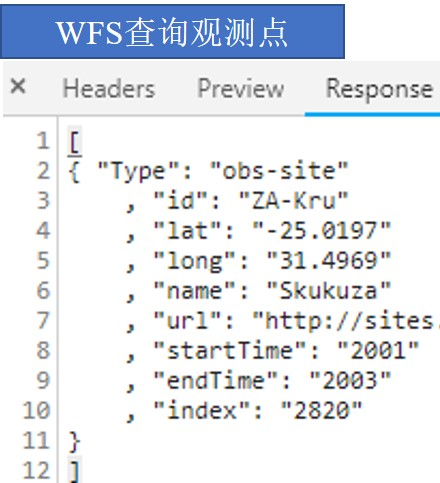
\includegraphics[width=0.42\textwidth]{wfs-example}}
    \hfill
    \subcaptionbox{WCS请求\label{fig:wcs-example}}{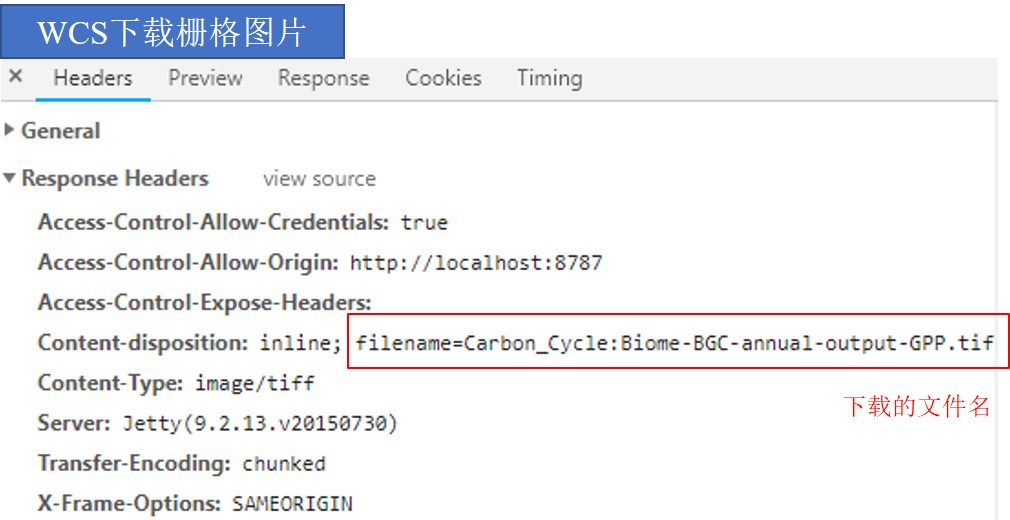
\includegraphics[width=0.52\textwidth]{wcs-example}}

    \caption{WFS和WCS}
    \label{fig:wfs-wcs}
\end{figure}

\subsubsection{数据下载服务}
数据下载服务主要是针对图~\ref{fig:data-arrange}设计的数据编排方式,在数据下载时,对数据路径规则进行反编码,查询到具体的数据条目,并通过HTTP协议返回给用户。

% \begin{figure}[!htbp]
%     \centering

%     \subcaptionbox{数据上传服务\label{fig:data-upload-service}}{\includegraphics[width=0.4\textwidth]{data-upload-service}}
%     \hfill
%     \subcaptionbox{数据下载服务\label{fig:data-download-service}}{\includegraphics[width=0.4\textwidth]{data-download-service}}

%     \caption{数据上传下载服务}
%     \label{fig:wms-example}
% \end{figure}

\subsubsection{数据处理服务}
% schema 匹配
% 数据抽取
% 数据重组
% 单位量纲
如图~\ref{fig:data-process-service}所示,本文用到的数据处理服务有三个:
\begin{enumerate}[(1)]
    \item \textbf{单位量纲转换服务}
    
    IBIS、Biome-BGC、LPJ三个模型的输出项单位不完全相同,比如GPP的单位有$gC m^{-2} d^{-1}$、$kgC m^{-2} d^{-1}$、$kgC m^{-2} a^{-1}$等,单位量纲转换服务以单位量纲资源库为参考,对三个模型输出数据项进行统一单位。

    \item \textbf{数据抽取服务}
    
    模型输出的数据步长是1天,而观测数据的时间范围往往有1-10年,时间序列过长,而且日间隔的数据噪点过多,通过数据抽取服务可以对数据进行平滑处理。
    
    \item \textbf{数据重组服务}
    
    模型输出数据是网格点的CSV数据,对于全球范围的数据可视化处理起来不够方便,因此使用数据重组服务将全球40595个格点的数据重组到一起,得到一个NetCDF数据。

\end{enumerate}

\begin{figure}[!htbp]
    \centering
    \subcaptionbox{单位量纲转换服务}{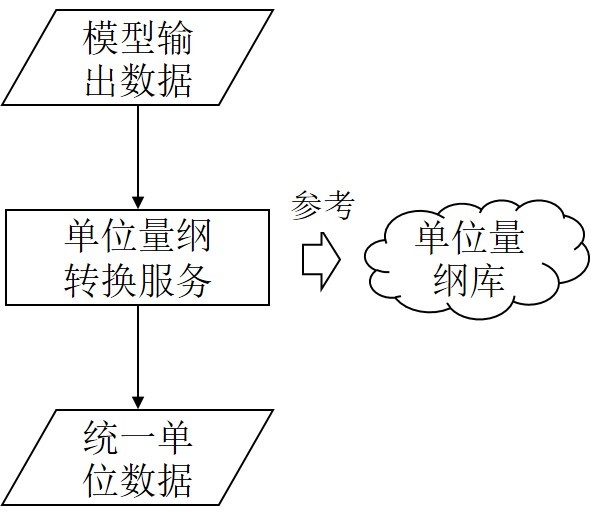
\includegraphics[width=0.4\textwidth]{data-service-1}}
    \hfill
    \subcaptionbox{数据抽取服务}{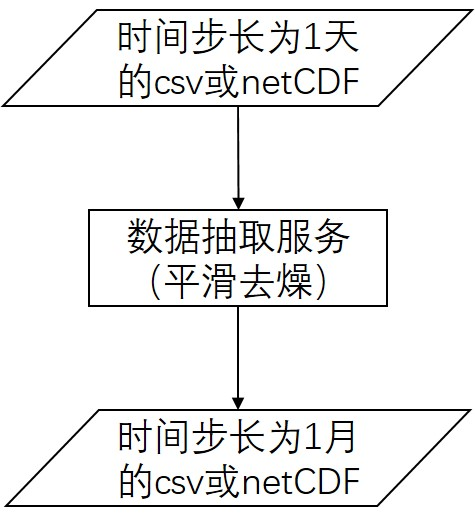
\includegraphics[width=0.25\textwidth]{data-service-2}}
    \hfill
    \subcaptionbox{数据重组服务}{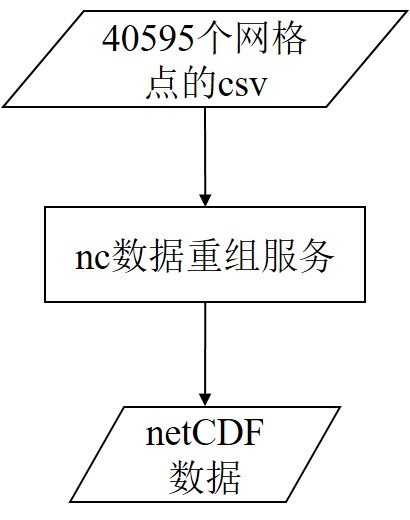
\includegraphics[width=0.25\textwidth]{data-service-3}}
    \caption{数据处理服务}
    \label{fig:data-process-service}
\end{figure}

% TODO
% \begin{figure}[!htbp]
%     \centering

%     \subcaptionbox{服务列表\label{fig:data-service-list}}{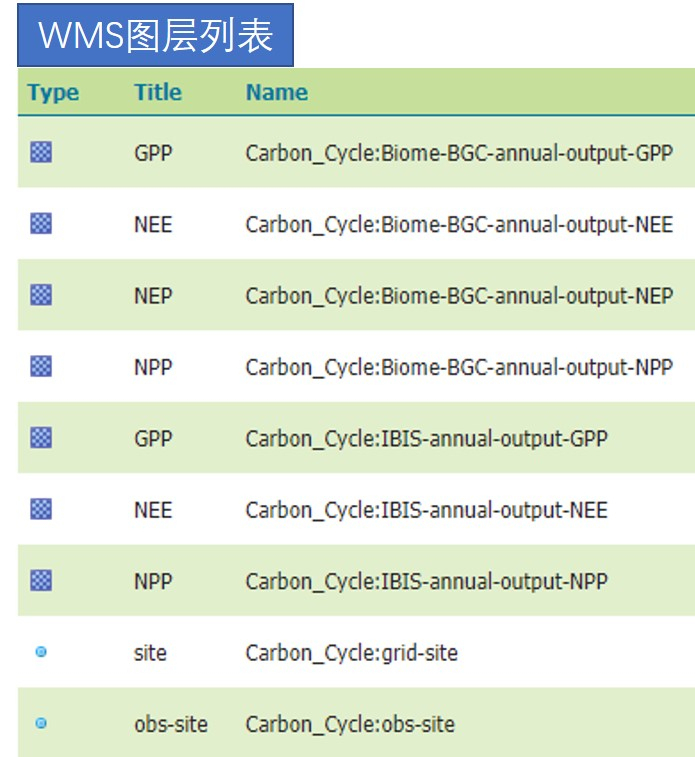
\includegraphics[width=0.4\textwidth]{wms-layers}}
%     \hfill
%     \subcaptionbox{服务调用\label{fig:data-service-invoke}}{\includegraphics[width=0.4\textwidth]{wms}} \\
%     \subcaptionbox{输入数据\label{fig:data-service-input}}{\includegraphics[width=0.4\textwidth]{wms}}
%     \hfill
%     \subcaptionbox{输出数据\label{fig:data-service-output}}{\includegraphics[width=0.4\textwidth]{wms}}

%     \caption{数据处理服务}
%     \label{fig:wms-example}
% \end{figure}


\section{开放式碳循环模型资源接入方法}
\label{sec:model-joinup}
如图~\ref{fig:ms-step}所示,模型资源的接入主要由模型描述、服务封装、服务部署和服务发布四步组成,下文将按照这个步骤介绍模型资源的接入方法。

\begin{figure}[!htbp]
    \centering
    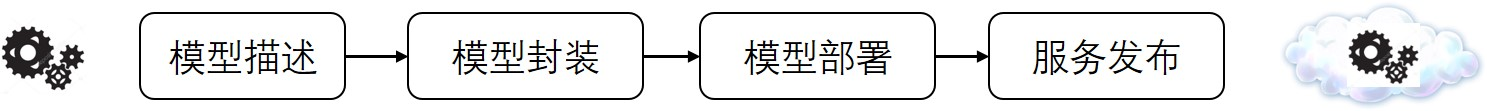
\includegraphics[width=1\textwidth]{ms-step}
    \caption{模型资源的服务化接入流程}
    \label{fig:ms-step}
\end{figure}

\subsection{碳循环模型资源异构特征分析}
% 碳循环模型存在着很强的异构性,其开发语言、运行平台、表现形式和集成过程各不相同,具体如表~\ref{tab:model-language-classify}所示(本文暂不考虑需要用户交互的模型)。所以
% 从运行角度,模型的异构性最明显的体现在其输入输出接口上,

地理模型的发展和信息技术紧密相关,模型作为可执行应用程序的一种,其异构性有很多体现在其运行特征上,包括:
\begin{enumerate}[(1)]
    \item \textbf{开发语言:}分为编译型和解释型,编译型包括C、C++、C\#、Fortran、Java等,解释型包括Python、MATLAB、JavaScript等。解释型语言在运行是需要解释器环境;
    \item \textbf{运行平台:}包括Windows、Linux和Unix等;
    \item \textbf{表现形式:}包括源代码、可执行程序、动态链接库、静态链接库、网络服务;
    \item \textbf{执行流程:}分为简单类型和复杂类型,简单类型不需要集成,复杂类型由多个子过程组成,运行时需要集成;
    \item \textbf{运行接口:}模型的数据读取方式各异,可以简单分为硬耦合方式、配置文件方式和命令行参数三种,每一类下又存在不同的具体标准,如图~\ref{fig:before-encap},IBIS、Biome-BGC和LPJ的运行接口各不相同,其中IBIS和LPJ通过源代码硬耦合的方式,这种方式在更换数据时需要重新编译,极其不便;Biome-BGC通过将输入数据写在配置文件中,比硬耦合的方式更加灵活,但是不同模型的配置方式往往不同,很难定义统一标准。
    \begin{figure}[!htbp]
        \centering
        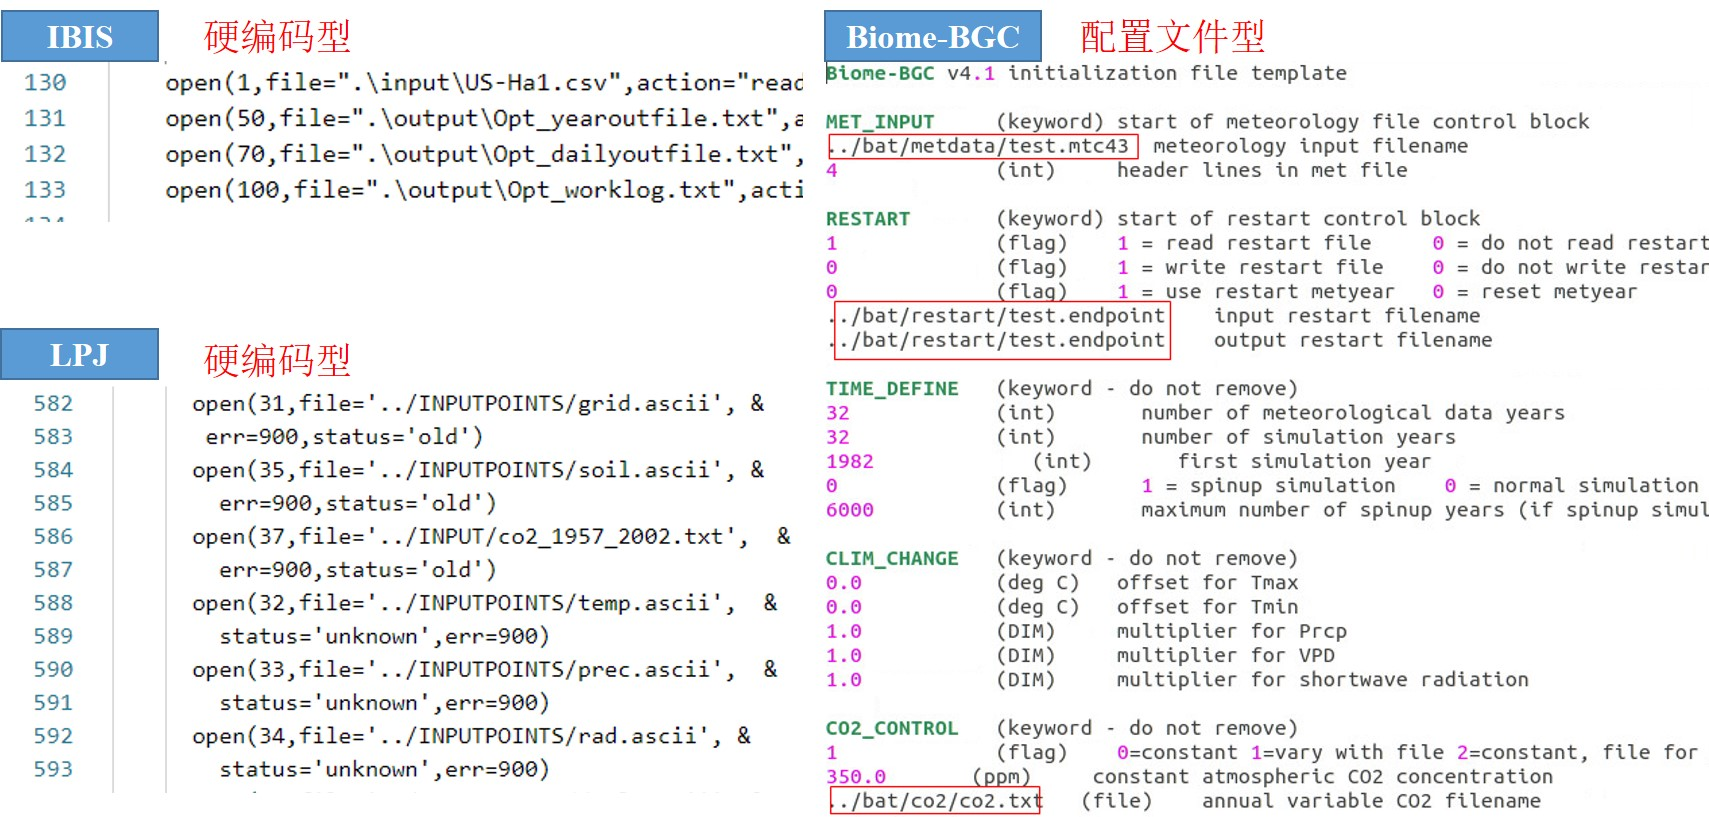
\includegraphics[width=1\textwidth]{before-encap}
        \caption{IBIS、Biome-BGC和LPJ的运行接口}
        \label{fig:before-encap}
    \end{figure}
\end{enumerate}

针对这些运行方面的异构性,模型封装时只有屏蔽这些特征,才能以统一的方式接入到对比框架中。

% \begin{table}
%     \centering
%     \caption{模型的异构性}
%     \label{tab:model-language-classify}
%     \begin{threeparttable}
%         \begin{tabular}{l | l l}
%             \Xhline{1.5pt}
%             分类标准 & 一级分类 & 二级分类 \\
%             \Xhline{1.5pt}
%             \multirow{8}{*}{语言} & \multirow{5}{*}{编译型} & C \\
%             & & C++ \\
%             & & C\# \\
%             & & Fortran \\
%             & & Java \\
%             \cline{2-3}
%             & \multirow{3}{*}{解释型} & Python\\
%             & & MATLAB \\
%             & & JavaScript \\
%             \hline
%             \multirow{3}{*}{平台} & Windows & \\
%             & Linux & \\
%             & Unix & \\
%             \hline
%             \multirow{3}{*}{交互} & 无交互 & \\
%             & 图形用户界面交互 & \\
%             & 控制台用户界面交互 & \\
%             \hline
%             \multirow{5}{*}{表现形式} & 源代码 & \\
%             & 可执行程序 & \\
%             & 动态链接库 & \\
%             & 静态链接库 & \\
%             & 网络服务 & \\
%             \hline
%             \multirow{2}{*}{集成} & 不需集成 & \\
%             & 由多步组成,需要集成 & \\
%             \Xhline{1.5pt}
%         \end{tabular}
%     \end{threeparttable}
% \end{table}

\subsection{碳循环模型资源描述方法}
\label{sec:ms-desc}
对模型资源的异构性特征进行结构化描述表达是模型服务化封装发布的基础,模型服务描述文档应该是面向人的,通过模型服务描述文档提供的信息,模型服务使用者就能够方便地了解和使用模型,并能够理解模型的返回结果;同时模型服务描述文档又是面向机器的,通过模型服务描述文档提供的模型运行输入输出选项,能够判断出模型运行数据的完备性,并在用户发送请求时将模型调用起来。因此,本文将模型服务的描述文档设计为如图~\ref{fig:mdl}。其中AttributeSet表示基本信息描述接口,面向人的理解;Process表示模型的运行接口信息,面向机器对模型的调用;Dependencies表示模型的软硬件环境依赖,也是面向机器,表示模型所依赖的软硬件环境信息。

% 模型服务描述的难点在于对于模型依赖数据的结构的有效表达和对于运行输入输出的合理描述。对于前者,本文采用第~\ref{sec:data-desc}的方法,即采用领域通用标准数据的描述加上示例数据具体展示的形式,对于后者,将在第~\ref{sec:io-interface}节介绍。


% 模型描述文档由JSON形式表达,与本文选择的具体技术体系有关:一方面它与MongoDB数据库结构同构,可以直接存储于数据库中,有助于增删查改,另一方面它与后台服务器Node.js天生兼容,解析起来方便。

\begin{figure}[!htbp]
    \centering
    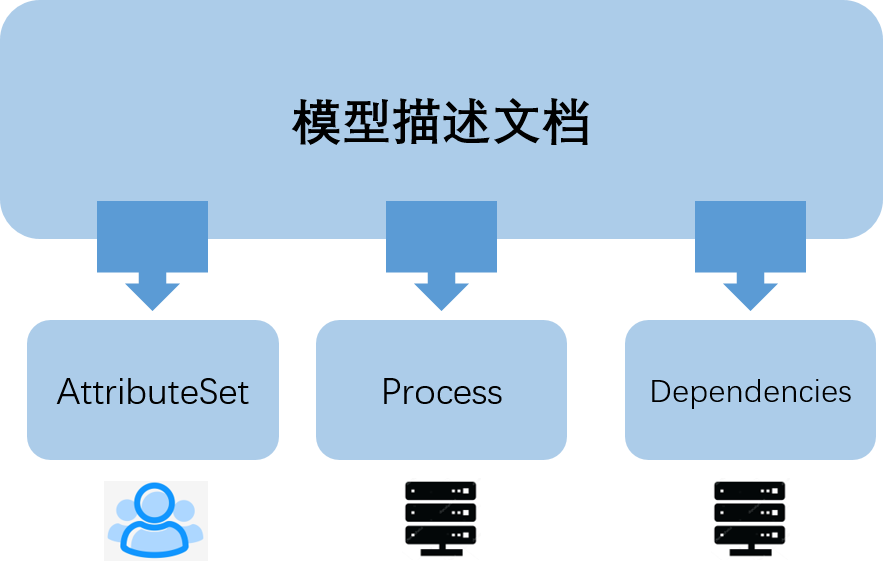
\includegraphics[width=.5\textwidth]{mdl}
    \caption{模型描述文档设计}
    \label{fig:mdl}
\end{figure}

\begin{enumerate}[(1)]
\item \textbf{基本信息描述接口设计}

基本信息的描述如图~\ref{fig:ModelCalculation!4-2-1-model-description-interface_1}所示,包括模型名称、作者、关键字、所属分类体系、DOI、wiki和计算节点信息。其中计算节点信息描述了模型服务的IP、端口和路由前缀等信息,从而在模型请求时能够解析出对应的URL。而wiki的设定允许模型服务使用者也能够维护模型服务的介绍,在经过模型服务拥有者的审核后,会补充到模型服务的描述文档中,这样就可以弥补描述接口的不足之处。

\begin{figure}[!htbp]
    \centering
    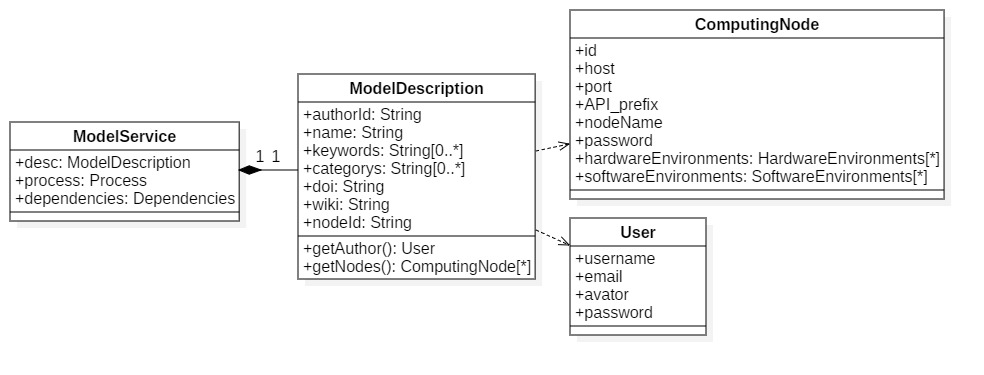
\includegraphics[width=1\textwidth]{jpg/ModelCalculation!4-2-1-model-description-interface_1}
    \caption{基本信息描述接口设计}
    \label{fig:ModelCalculation!4-2-1-model-description-interface_1}
\end{figure}

\item \textbf{运行信息描述接口设计}
\label{sec:io-interface}
% 存储路径、文件名、类型(编译、解释)、
% 两个粒度:单模型运行和多模型集成

运行信息的描述接口如图~\ref{fig:ModelCalculation!4-2-2-model-invoke-interface_0}所示,包括模型的可执行程序文件名、程序类型、解释器类型、输入数据、输出数据和参数(本文将文件型的数据称为输入数据,将Number或String型的数据称为参数)以及各种数据的结构化元数据描述。本文将模型从开发语言上分为编译型和解释型两种,对于解释型的语言,需要记录模型的解释器,在运行时通过解释器调用才能运行。通过运行信息的描述,可以在用户调用时执行execute()函数,并返回子进程的pid,在需要时可以通过kill(pid)函数杀死进程。

\begin{figure}[!htbp]
    \centering
    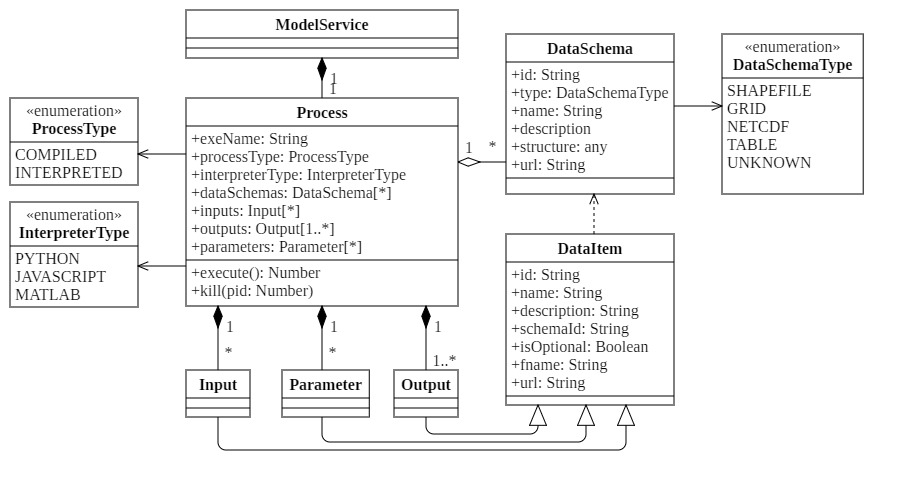
\includegraphics[width=1\textwidth]{jpg/ModelCalculation!4-2-2-model-invoke-interface_0}
    \caption{运行信息描述接口设计}
    \label{fig:ModelCalculation!4-2-2-model-invoke-interface_0}
\end{figure}

\item \textbf{部署信息描述接口设计}

部署信息的描述接口如图~\ref{fig:ModelCalculation!4-2-3-model-deployment-interface_2}所示,包括模型运行所需的软件和硬件依赖环境。通过与计算节点的软硬件环境数据库相匹配可以得到部署环境是否匹配,当环境相匹配时才能调用成功。

\begin{figure}[!htbp]
    \centering
    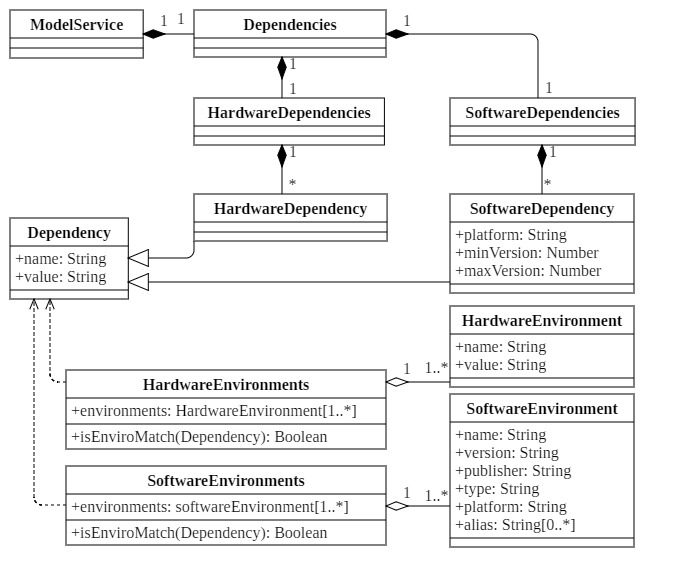
\includegraphics[width=1\textwidth]{jpg/ModelCalculation!4-2-3-model-deployment-interface_2}
    \caption{部署信息描述接口设计}
    \label{fig:ModelCalculation!4-2-3-model-deployment-interface_2}
\end{figure}
\end{enumerate}

\subsection{碳循环模型资源的服务化}
\label{subsec:ms-encap}
\subsubsection{模型封装}
% 接口设计
% 几种方式:模型代理、源码封装
% 对于执行链的封装

在计算机领域,封装是对实体进行包装或组合形成具有稳定接口的新实体的方法和技术~\cite{2015-hudi-2}。通过封装,可以屏蔽原有程序的实现细节,提高模型的可复用性和可维护性,降低用户的使用难度。封装可以体现在程序设计的各个层次上,如函数、类、模块、组件、系统、可执行程序和Web服务这些粒度上都可以进行封装,本文的封装将模型包装成具有标准接口的控制台应用程序。

模型封装最关键的是运行接口的设计,而模型运行接口的设计本质上是设计一个命令行参数解析标准,将输入输出选项映射给程序内存变量,业界有很多成熟的标准,如libc的getopt/getopt\_long接口、google的gflags接口等。本文采用的getopt/getopt\_long接口,它在很多其他语言上都有对应的移植版本,方便对不同语言模型封装的实现。getopt/getopt\_long接口支持单字符选项、多字符选项和可选参数选项,可以方便地生成帮助信息。通过getopt/getopt\_long的标准化,模型的调用命令可表示为“exeName -a -i=``filepath1'' -p=``10'' -o=``filepath3''”或“exeName -a --inputFile1=``filepath2'' --parameter1=``10'' --outputFile1=``filepath3''”。其中选项列表来自于运行信息描述文档,以“-”开头表示单字符选项,以“--”开头表示多字符选项,不带等号的如“-a”为参数选项。对于IBIS的封装,标准化后调用方式可表示为“IBIS --meteorology="meteorology\_file\_path" --soil="soil\_file\_path" --output="output\_file\_save\_path"”。对于解释型的语言,需要在命令前面加上解释器,如Biome-BGC模型的调用方式可表示为“node Biome-BGC.js -a --ini="ini\_config\_path" --met="meteorology\_file\_path" --co2="co2\_file\_path" --epc="PFT\_parameters\_file\_path" --output="output\_file\_path"”。

模型封装根据有无源码可以分为基于源码的封装和基于模型代理的封装,如图~\ref{fig:source-encap-proxy-encap}所示,源码封装直接对模型输入输出接口做出修改使其标准化,模型代理封装通过写一个模型代理壳将其IO标准化,然后通过fork子进程启动模型完成封装。按照模型是否包含集成分为简单模型封装和包含集成流程的模型的封装。Biome-BGC模型的执行过程分为spin-up模式和正常模式两步,正常模式的运行依赖于spin-up模式,整个运行过程中有一个简单的串联集成过程,如图~\ref{fig:ms-encap-with-integration}所示,通过Node.js脚本可以非常方便的串联集成。

\begin{figure}[!htbp]
    \centering
    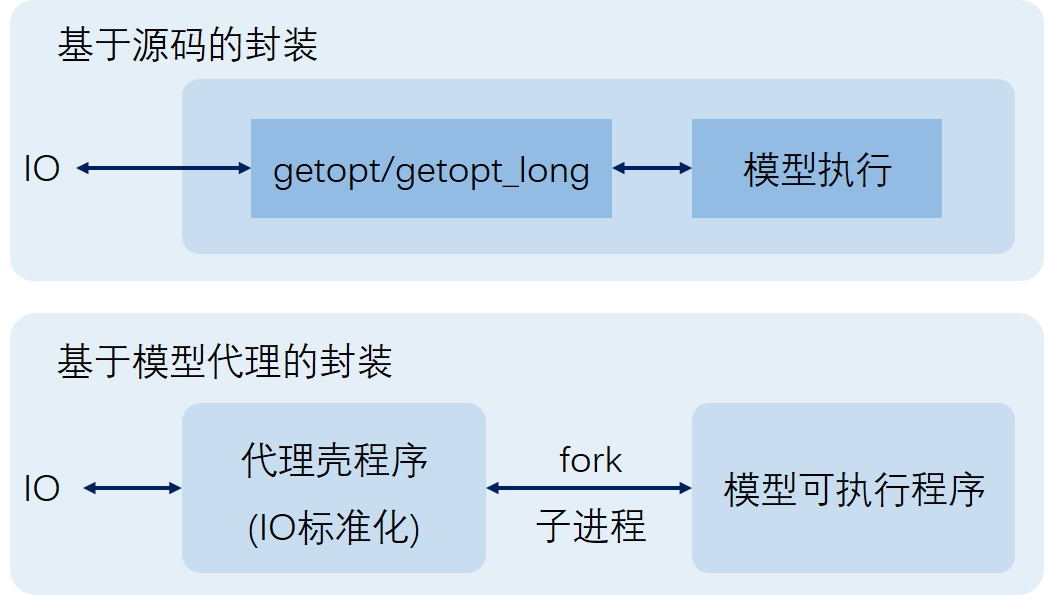
\includegraphics[width=.8\textwidth]{source-encap-proxy-encap}
    \caption{基于源码的封装和基于模型代理的封装}
    \label{fig:source-encap-proxy-encap}
\end{figure}

\begin{figure}[!htbp]
    \centering
    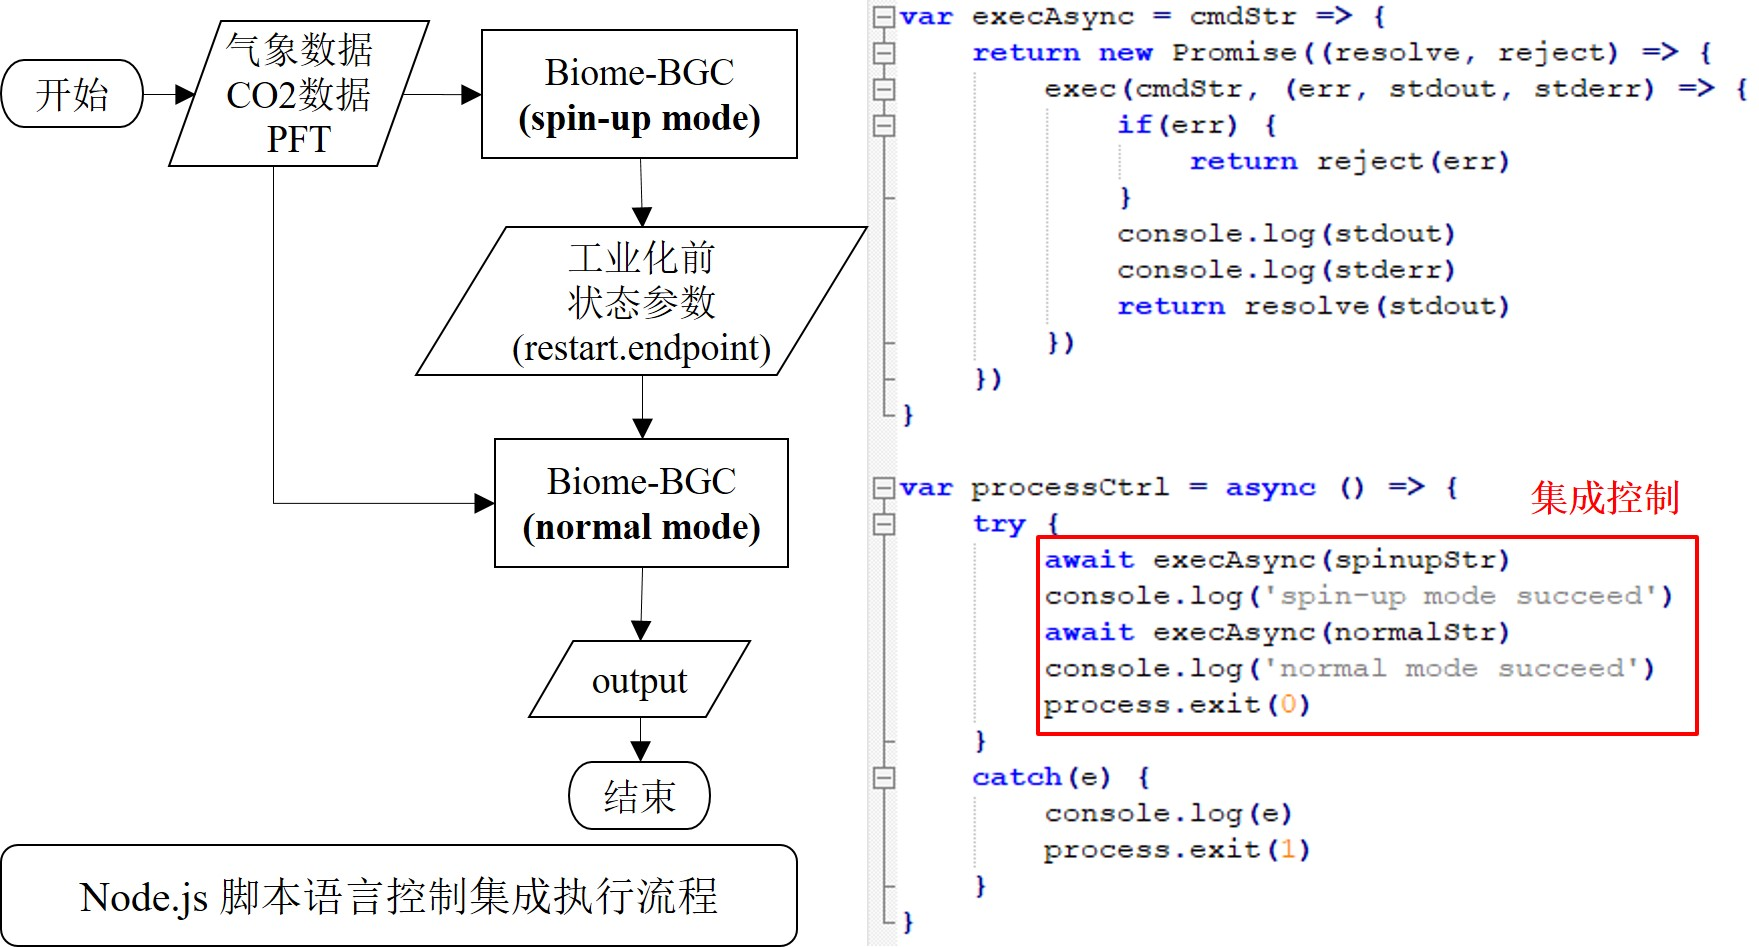
\includegraphics[width=1\textwidth]{ms-encap-with-integration}
    \caption{模型的串联集成封装,以Biome-BGC为例}
    \label{fig:ms-encap-with-integration}
\end{figure}

如图~\ref{fig:after-encap}所示,IBIS、Biome-BGC和LPJ三个模型封装后的调用方式一致,可以概括为``(interpreter) <main> -p -f=<value> --flag=<value>''。其中``interpreter''为解释器,当程序语言是解释型的时候才需要,“main”是入口程序名,“-p”是参数标识,“-f”是短标识,“--flag”是长标识。参数标识、短标识和长标识在模型运行描述文档中具体体现。

\begin{figure}[!htbp]
    \centering
    \includegraphics[width=1\textwidth]{after-encap}
    \caption{IBIS、Biome-BGC和LPJ封装后的运行接口}
    \label{fig:after-encap}
\end{figure}


\subsubsection{服务部署和发布}
% 数据库录入条目、服务部署
% 运行环境
服务部署和发布是将封装好的模型程序迁移到目标计算节点上的过程,主要包括模型服务描述文档数据库条目的录入和模型运行软硬件环境的匹配。对于模型服务描述文档,本文将数据库设计与第\ref{sec:ms-desc}节的描述接口同构,可以直接录入。对于软件环境,IBIS和LPJ使用gfortran编译的,需要libgfortran的动态链接库;Biome-BGC使用gcc编译,其依赖的软件环境libc是linux系统的底层接口,不需要重新安装。对于硬件环境,本文所用的三个模型对硬件要求都不高,可以直接部署在普通PC机上。

\section{开放式碳循环对比资源接入方法}
% 对比方案的 构建=》执行(网络消息传送)=》结果
% 对比方案的结构化描述、资源映射、服务化
\subsection{碳循环模型对比方法}
\subsubsection{统计学对比方法}
\begin{align}
    &SD = \sqrt{\frac{\sum\limits_{i=1}^{N}\left(x_i-\bar{x_i}\right)^2}{N}}
    \label{eq:SD} \\
    &SSE = \sum\limits_{i=1}^{N}\left(y_i-\hat{y_i}\right)^2 \\
    &SST = \sum\limits_{i=1}^{N}\left(y_i-\bar{y_i}\right)^2 \\
    &MSE = \frac{SSE}{n} \\
    % &MSE_S = \frac{}{N}
    % \label{eq:MSE-S} \\
    % &MSE_U = \frac{}{N}
    % \label{eq:MSE-U} \\
    &RMSE = \sqrt{MSE} = \sqrt{\frac{\sum\limits_{i=1}^{N}\left(y_i-\hat{y_i}\right)^2}{N}}
    \label{eq:RMSE}  \\
    % &RMSE_r = \sqrt{\frac{\sum\limits_{_i=1}^{N}\left[\left(y_i-\hat{y_i}\right)/\bar{y}\right]^2}{N}} \times 100\%
    % \label{eq:RMSE-R} \\
    &R^2 = \frac{SSR}{SST} = 1 - \frac{SSE}{SST} = 1 - \frac{\sum\limits_{i=1}^{N}\left(y_i-\hat{y_i}\right)^2}{\sum\limits_{i=1}^{N}\left(y_i-\bar{y_i}\right)^2}
    \label{eq:R^2} \\
    &NSE = 1 - \frac{\sum\limits_{t=1}^{T}\left(Q_o^t - Q_m^t\right)^2}{\sum\limits_{t=1}^{T}\left(Q_o^t - \bar{Q_o}\right)^2}
    \label{eq:NSE}
\end{align}
本文主要用以下几个统计变量评价IBIS、Biome-BGC、LPJ三个模型在网格点的模拟准确度:
\begin{enumerate}[(1)]
\item \textbf{标准差(Standard Deviation,记为$SD$)}

标准差又称均方差,用来表示一组数据的离散程度,如公式~\ref{eq:SD}所示。

\item \textbf{均方根误差(Root Mean Square Error,记为$RMSE$)}

均方根误差又称标准误差,表示有限观测数据中,观测值与真值的偏差。本文使用均方根误差表示网格点模拟值与观测值的偏差,从而反映模型的模拟能力。均方根误差可表示为公式~\ref{eq:RMSE},其中$RMSE$表示均方根误差,$MSE$表示均方误差,$y_i(i=1,2,...,N)$为观测数据,$\hat{y_i}$为预测数据。

\item \textbf{决定系数(记为$R^2$)}

决定系数反映因变量的全部变异能通过回归关系被自变量解释的比例,其公式如~\ref{eq:R^2}所示。

\item \textbf{效率系数(Nash-Sutcliffe coefficient,记为$NSE$)}

效率系数用来评价模型模拟的好坏~\cite{gordon2003climate},如公式~\ref{eq:NSE}所示,式中,$Q_o$指观测值,$Q_m$指模拟值,$Q^t$指第t时刻的某个值,$\bar{Q_o}$表示观测值的平均值。$NSE$等于1减去均方误差与观测值变异的比值。$NSE$值的范围从负无穷大到1,越接近1表示模型效果越好。如果模拟值的均方误差与观测值的方差相同,则$NSE$等于0;如果模拟值的均方误差大于观测值的方差,则$NSE$小于0;如果模拟值的均方误差小于观测值的方差并趋近于后者,则$NSE$趋近于1,表示模型具有很好的模拟能力。

\item \textbf{超级集合}

超级集合由Krishnamuti~\cite{krishnamurti1999improved}等提出,通过多元线性回归分析对每个观测站点的数据进行分析,各模型的权重系数,如公式~\ref{eq:SE}所示:

\begin{align}
    &F_t = \bar{O} + \sum\nolimits_{i=1}^{N}a_i\left(F_{i,t}-\bar{F_t}\right)
    \label{eq:SE}
\end{align}

式中,$F_t$是超级集合合成后的预测值;$\bar{O}$是训练期的平均观测值;$F_{i,t}$是第$i$个模型的预测值;$\bar{F_t}$是第$i$个模式在训练期的平均预测值;$n$是参加建立超级集合的模型数量;$t$是时间;$a_i$是回归系数,代表各个模型的权重。在建立超级集合时,将数据分成训练集和验证集,通过训练集获取式中的各个参数,通过验证集验证超级集合的模拟水平。本文中参与建立超级集合的模型有MODIS MOD17 A3、IBIS、Biome-BGC、LPJ,观测值数据是FLUXNET 2015,具体对比结果见第~\ref{sec:experiments}节。

\end{enumerate}

\subsubsection{可视化对比方法}
\begin{figure}[!htbp]
    \centering
    \subcaptionbox{泰勒图\label{fig:example-taylor}}{\includegraphics[width=0.47\textwidth]{example-taylor}}
    \hfill
    \subcaptionbox{时间序列折线图\label{fig:example-timeseries-diagram}}{\includegraphics[width=0.47\textwidth]{example-timeseries-diagram}} \\ 
    \subcaptionbox{地图\label{fig:example-raster-map}}{\includegraphics[width=0.7\textwidth]{raster-map}}\\
    \subcaptionbox{热力图\label{fig:example-heatmap}}{\includegraphics[width=0.47\textwidth]{heatmap-GPP-coef}}
    \hfill
    \subcaptionbox{纬向图\label{fig:example-lat}}{\includegraphics[width=0.47\textwidth]{GPP-lat}}
    \caption{可视化对比图表}
    \label{fig:ms-server-microservice}
\end{figure}
\begin{enumerate}[(1)]
\item \textbf{泰勒图}

泰勒图常用于评价模型的精度,如图~\ref{fig:example-taylor}所示,泰勒图中的散点表示模型,辐射线表示相关系数,横轴线表示标准差,虚线表示均方根误差~\cite{taylor2001summarizing},泰勒图能够在二维平面上同时呈现三个指标,在IPCC、CMIP5、CMIP6中被广泛应用于多模型模拟能力评估对比。

\item \textbf{时间序列折线图}

如图~\ref{fig:example-timeseries-diagram}所示,时间序列折线图反映的是模拟指标的年际或季节变化趋势,能够直观地显示观测指标的走向。

\item \textbf{热力图}

如图~\ref{fig:example-heatmap}所示,横轴是模型,纵轴是观测站点,横着看能直观地发现不同模型对同一个站点的模拟能力差异,纵着看能直观地发现同一个模型在不同站点的模拟能力差异。

\item \textbf{地图}

如图~\ref{fig:example-raster-map}所示,分别是等值线图和偏差等值线图,等值线图可以直观地表现GPP的空间分布格局,偏差等值线图则表示的是模型误差的空间分布。

\item \textbf{纬向图}

如图~\ref{fig:example-lat}所示,纬向图横轴是纬度,纵轴是观测指标,可以展示出观测指标的纬度分布规律。

\end{enumerate}

\subsection{对比方法接入方法}
对比方法实质上是数据处理脚本,它以数据重构方法转换过的数据为输入项,对其进行统计学或可视化分析,并输出统计指标和图片。因此,对比方法可以采用和模型一致的封装方法,包括以下几步实现:

\begin{enumerate}[(1)]
    \item 对比方法的脚本实现。本文选择python的科学计算发行版conda作为开发语言,conda有非常便利的CSV和NETCDF第三方数据解析库pandas和netcdf4,以及图表可视化库matplotlib、seaborn和basemap,对于统计数据处理也非常方便。在编写实现脚本时,通过python的getopt对输入输出项进行标准化,就免去了模型封装的步骤;
    \item 对比脚本的结构化文档描述。与模型描述方法完全相同;
    \item 对比方法的部署、发布。与模型描述方法完全相同。
\end{enumerate}

\section{本章小结}
本章针对数据、模型和对比方法这三种对比资源在框架下的开放式服务化接入进行了详细的阐述。对于数据资源,从数据格式、尺度、编排三个角度分析了其特征,通过本文设计的数据描述语言来描述NetCDF、Shapefile和CSV数据,实现了OGC WMS、WFS、WCS、数据下载服务、数据重构服务的发布;对于模型资源,分析了其异构性特征,设计了面向人和机器理解的模型描述接口,并通过运行接口的设计实现了模型服务的封装、部署和发布;对于对比方法,详细介绍了本文用到的统计学对比方法和可视化对比方法,并采用模型封装接口将对比方法也封装为开放式服务资源。
\chapter{原型系统与案例验证}

\section{原型系统构建}
\subsection{网络架构和系统功能模块设计}
\subsection{陆地生态系统碳循环对比资源库}
\subsection{开放式对比任务执行引擎}

\section{实验案例}
\subsection{模型资源和数据资源}
\subsection{对比方案}
\subsection{对比结果}
\chapter{结论与展望}

\section{研究结论}
% 系统方面的结论:系统的可用性;可扩展性
% 陆地碳循环方面的结论
\section{创新点}
\section{不足与展望}
\subsection{不足}
\subsection{展望}


%%% 其它部分
\backmatter

% %% 本科生要这几个索引,研究生不要。选择性留下。
% % 插图索引
% \listoffigures
% % 表格索引
% \listoftables
% % 公式索引
% \listofequations


%% 参考文献
% 注意:至少需要引用一篇参考文献,否则下面两行可能引起编译错误。
% 如果不需要参考文献,请将下面两行删除或注释掉。
% 数字式引用
\bibliographystyle{thuthesis-numeric}
% 作者-年份式引用
% \bibliographystyle{thuthesis-author-year}
\bibliography{ref/refs}


%% 致谢
% % 如果使用声明扫描页,将可选参数指定为扫描后的 PDF 文件名,例如:
% \begin{acknowledgement}[scan-statement.pdf]
\begin{acknowledgement}
  衷心感谢导师 xxx 教授和物理系 xxx 副教授对本人的精心指导。他们的言传身教将使
  我终生受益。
\end{acknowledgement}


%% 附录
% \begin{appendix}
% \chapter{在读期间发表的学术论文及科研情况}

\noindent{\textbf{申请的软件著作权:}}
\begin{enumerate}
    \item \textbf{沈超然}、张丰源、侯涛、陈坤、乐松山、陈旻.分布式地理建模平台模型服务容器软件.2017SR603822
    \item 张博文、谭羽丰、\textbf{沈超然}、侯涛、乐松山、温永宁.地理数据服务与地理模型服务集成运行系统.2017SR422324
    \item 侯涛、朱串串、张博文、\textbf{沈超然}、乐松山、陈旻.地理模型资源的分类存储于动态部署软件.2017SR416517
\end{enumerate}

\par \qquad

\noindent{\textbf{主要获奖情况:}}
\begin{enumerate}
    \item 获得2016-2017学年一等学业奖学金
    \item 获得2017-2018学年三等学业奖学金
    \item 获得2018-2019学年一等学业奖学金
\end{enumerate}
% \end{appendix}

%% 个人简历
% \begin{resume}
  \researchitem{申请的软件著作权:}
  \begin{achievements}
    \item \textbf{沈超然}、张丰源、侯涛、陈坤、乐松山、陈旻.分布式地理建模平台模型服务容器软件.2017SR603822
    \item 张博文、谭羽丰、\textbf{沈超然}、侯涛、乐松山、温永宁.地理数据服务与地理模型服务集成运行系统.2017SR422324
    \item 侯涛、朱串串、张博文、\textbf{沈超然}、乐松山、陈旻.地理模型资源的分类存储于动态部署软件.2017SR416517
  \end{achievements}

  \researchitem{主要获奖情况:}
  \begin{achievements}
    \item 获得2016-2017学年一等学业奖学金
    \item 获得2017-2018学年三等学业奖学金
    \item 获得2018-2019学年一等学业奖学金
  \end{achievements}

\end{resume}


%% 本科生进行格式审查是需要下面这个表格,答辩可能不需要。选择性留下。
% 综合论文训练记录表
% \includepdf[pages=-]{scan-record.pdf}
\end{document}
